% Define document class
\documentclass[twocolumn]{aastex631}
\usepackage{showyourwork}

\newcommand{\sbu}{Department of Physics and Astronomy, Stony Brook University, Stony Brook NY 11794, USA}
\newcommand{\cca}{Center for Computational Astrophysics, Flatiron Institute, New York NY 10010, USA}
\renewcommand{\thefigure}{\arabic{figure}}

\usepackage{bbold}

% Begin!
\begin{document}

% Title
\title{Polka-dotted Stars: a Hierarchical Model for Mapping Stellar Surfaces Using Occultation Light Curves and the Case of TOI-3884}

% Author list
\author[0000-0002-6650-3829]{Sabina Sagynbayeva}
\email{sabina.sagynbayeva@stonybrook.edu}
\affiliation{\sbu}
\affiliation{\cca}
\affiliation{Kavli Institute for Theoretical Physics, University of California, Santa Barbara, CA 93106, USA}

\author[0000-0003-1540-8562]{Will M. Farr}
% \email{wfarr@flatironinstitute.org}
\affiliation{\sbu}
\affiliation{\cca}

\author[0000-0003-2528-3409]{Brett M. Morris}
% \email{wfarr@flatironinstitute.org}
\affiliation{Space Telescope Science Institute, 3700 San Martin Dr, Baltimore, MD 21218, USA}

\author[0000-0002-0296-3826]{Rodrigo Luger}
% \email{rodluger@gmail.com}
\affiliation{\cca}

% Abstract with filler text
\begin{abstract}
    We present \texttt{StarryStarryProcess}, a novel hierarchical Bayesian framework for mapping stellar surfaces using exoplanet transit light curves. 
    While previous methods relied solely on stellar rotational light curves -— which contain limited information about spot properties -- our approach leverages 
    planetary transits as probes of stellar surfaces. When a planet crosses a spot during transit, it creates a distinctive bump in the light curve that 
    directly reveals spot properties. Our model integrates planetary transit modeling with stellar variability analysis by combining 
    the spherical harmonic representation from \texttt{starry}, the probabilistic approach of \texttt{StarryProcess}, and a comprehensive 
    transit model that accounts for spot-crossing events. We demonstrate through synthetic data experiments that our model successfully recovers spot distributions, 
    stellar orientation, and spot physical properties. We extend the framework to handle evolving stellar surfaces through time-dependent modeling. 
    Applying our method to TESS observations of TOI-3884, we find evidence for high-latitude spot concentrations and significant spin-orbit misalignment. The transit-based 
    approach overcomes fundamental limitations of previous models by providing constraints on spot properties that would remain hidden in the null space of 
    rotational light curves alone. This methodology enables more accurate exoplanet characterization by disentangling stellar activity from planetary signals 
    while simultaneously providing insights into stellar magnetic activity patterns.
\end{abstract}

% Main body with filler text
\section{Introduction}
\label{sec:intro}
The detection of atmospheres on Earth analogs using transmission spectroscopy is challenging due to stellar 
contamination effects \citep{Ducrot2018, Morris2018}. Stellar magnetic activity, particularly starspots, significantly 
influences observed transmission spectra, making it difficult to distinguish planetary atmospheric signals from stellar ones. 
Starspots exhibit variations in both time and wavelength primarily due to stellar rotation, potentially complicating the analysis 
and interpretation of exoplanet observations.

Therefore, characterizing stellar surface features arising from magnetic activity—-such as starspots and flares—-is crucial for 
improving planet detection efficiency across photometric, spectral, and radial velocity studies. Understanding starspots is 
especially important for the JWST mission, which aims to characterize numerous exoplanet atmospheres around stars with strong 
variability. Recent JWST results on TRAPPIST-1b \citep{Lim2023} demonstrated that accurate measurements have been substantially 
hindered by stellar contamination, highlighting the need for more precise models to account for these effects. To fully leverage 
JWST's capabilities and accurately interpret transmission spectra, we must develop a comprehensive understanding of stellar 
magnetic activity and its impact on observed signals.

Recent works have provided valuable insights into the topographical characteristics of stars and their magnetic activity. 
For example, starspot influence can be observed through photometric data from Kepler or TESS. The \texttt{starry} code 
\citep{Luger2019} offers an efficient method for computing light curves of stars and planets using a spherical harmonic 
framework to represent surface brightness distribution, enabling fast and accurate calculations of rotational light curves 
and occultations. Building upon \texttt{starry}, \citet{Luger2021b} introduced \texttt{StarryProcess}, a probabilistic model 
for stellar variability that treats spot distribution as a Gaussian process in spherical harmonic space, allowing efficient 
modeling of stellar variability over extended time scales.

With \texttt{StarryProcess}, \citet{Luger2021b} investigated stellar spot features using Gaussian Processes with 
a physically interpretable kernel. They argued that complex degeneracies make it impossible to determine the precise 
configuration of starspots solely from rotational light curves. Instead, they suggested focusing on the statistical properties 
of spot distributions rather than individual spot characteristics. However, they also demonstrated that constraining starspot 
properties from a single star's light curve is difficult; an ensemble analysis of multiple stars is more informative.

While previous models like \texttt{StarryProcess} relied solely on stellar rotational light curves—which contain limited 
information about spot properties—our approach introduces a critical advancement: we leverage planetary transits as probes of 
stellar surfaces. Exoplanet host stars are \textit{uniquely suited} for photometric studies of starspot properties because:
(1) Planetary transits effectively scan different regions of the stellar disk;
(2) Transit light curves contain encoded information about the stellar surface and starspots;
(3) Spot-crossing events during transits provide direct constraints on spot brightness, size, and latitude.

This transit-based approach overcomes the fundamental limitation of previous models that analyzed stellar light curves alone, 
where too many degeneracies exist to precisely characterize spots. As illustrated in Figure \ref{fig:cartoon}, when a planet 
crosses a spot during transit, it creates a distinctive bump in the light curve that directly reveals spot properties.

In this work, we develop \texttt{StarryStarryProcess}, a novel framework that integrates planetary transit modeling with 
stellar variability analysis. Our model combines:
\begin{itemize}
    \item The spherical harmonic representation from \texttt{starry}
    \item The probabilistic approach of \texttt{StarryProcess}
    \item A comprehensive transit model that accounts for spot-crossing events
\end{itemize}

By simultaneously modeling stellar variability, spot distributions, and planetary transits, our approach disentangles 
spot effects from transit features, resulting in more accurate constraints on both stellar and planetary parameters. 
When modeling multiple transits alongside underlying stellar variability, we can better determine stellar inclination, 
obliquity, and spot distribution patterns.

Figure \ref{fig:nullspace} illustrates a key insight of our approach: while previous methods struggled with the null 
space problem (where many surface features don't affect the observable light curve), planetary transits effectively 
"carve out" paths on the stellar surface that reveal information otherwise hidden in the null space. The transit trajectory 
covers regions in the preimage component (observable) that would remain undetectable in conventional analysis.

Our paper is organized as follows: Section \ref{sec:model} presents the \texttt{StarryStarryProcess} model; 
Section \ref{sec:experiment1} presents results on non-evolving stellar surfaces; Section \ref{sec:experiment2} 
presents results on evolving surfaces; Section \ref{sec:toi3884} presents results on TESS data for TOI-3884; and finally,
 we discuss implications and assumptions in Section \ref{sec:discussion}.

\begin{figure}[hbt!]
    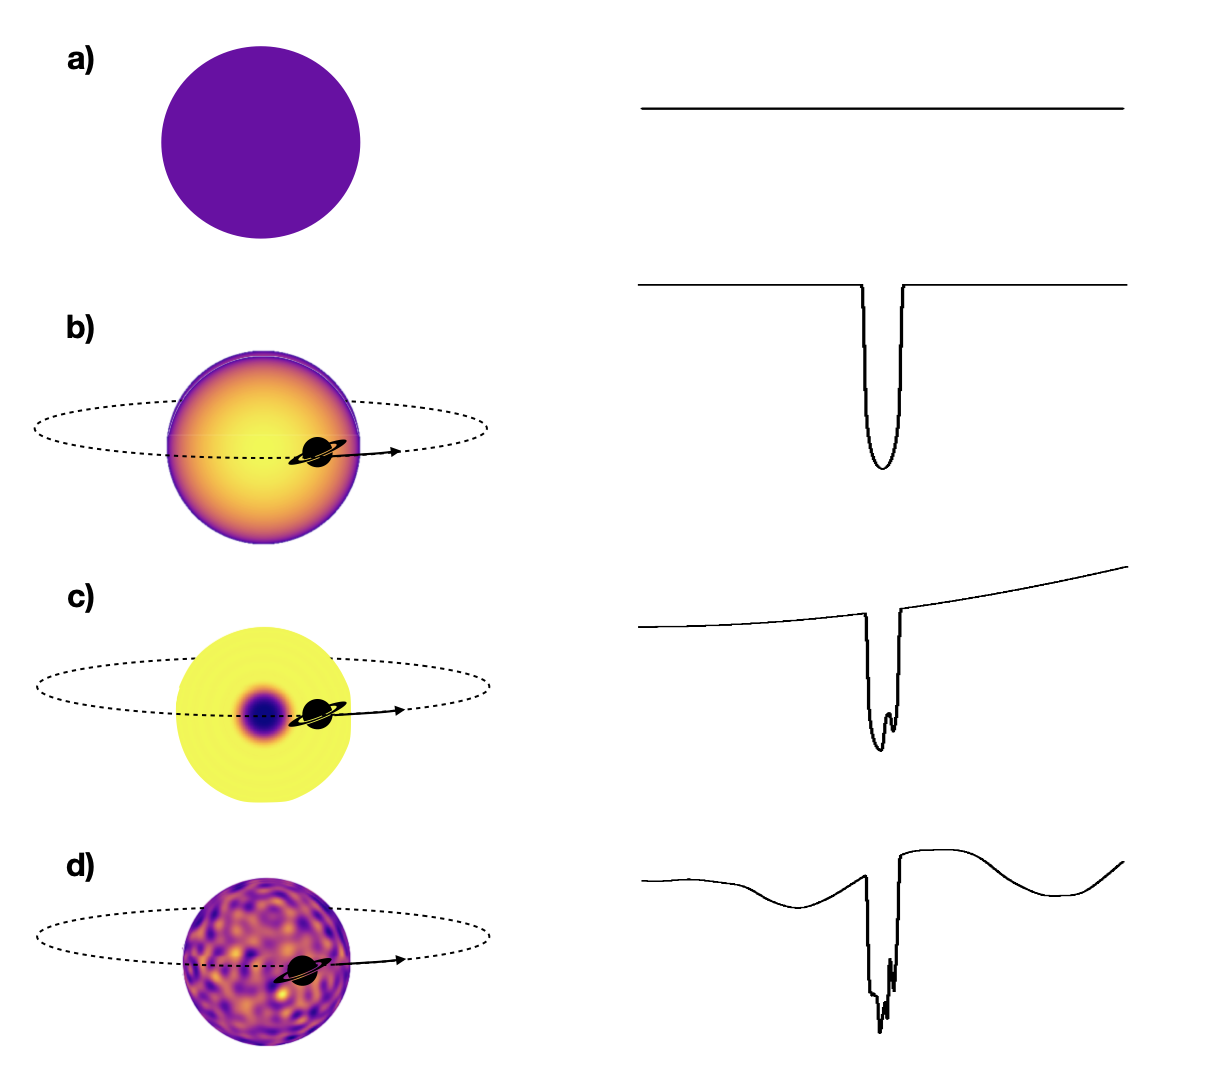
\includegraphics[width=0.46\textwidth]{figures/star-planet-cartoon.png}
        \caption{Light curves from the kinds of stars shown on the left panel (these light curves were calculated analytically 
        using \texttt{starry} \citep{Luger2019}): (a) the light curve shows a flat flux if the star has no surface features and no planet orbiting it; 
        (b) a transit in the light curve of the star that hosts an exoplanet; (c) if the star has one orbiting planet and one starspot under the planet's 
        trajectory then it is seen as a bump in a transit signal; (d) the light curve becomes complicated when the star has multiple spots.}
        \label{fig:cartoon}
    \end{figure}

\begin{figure*}[hbt!]
    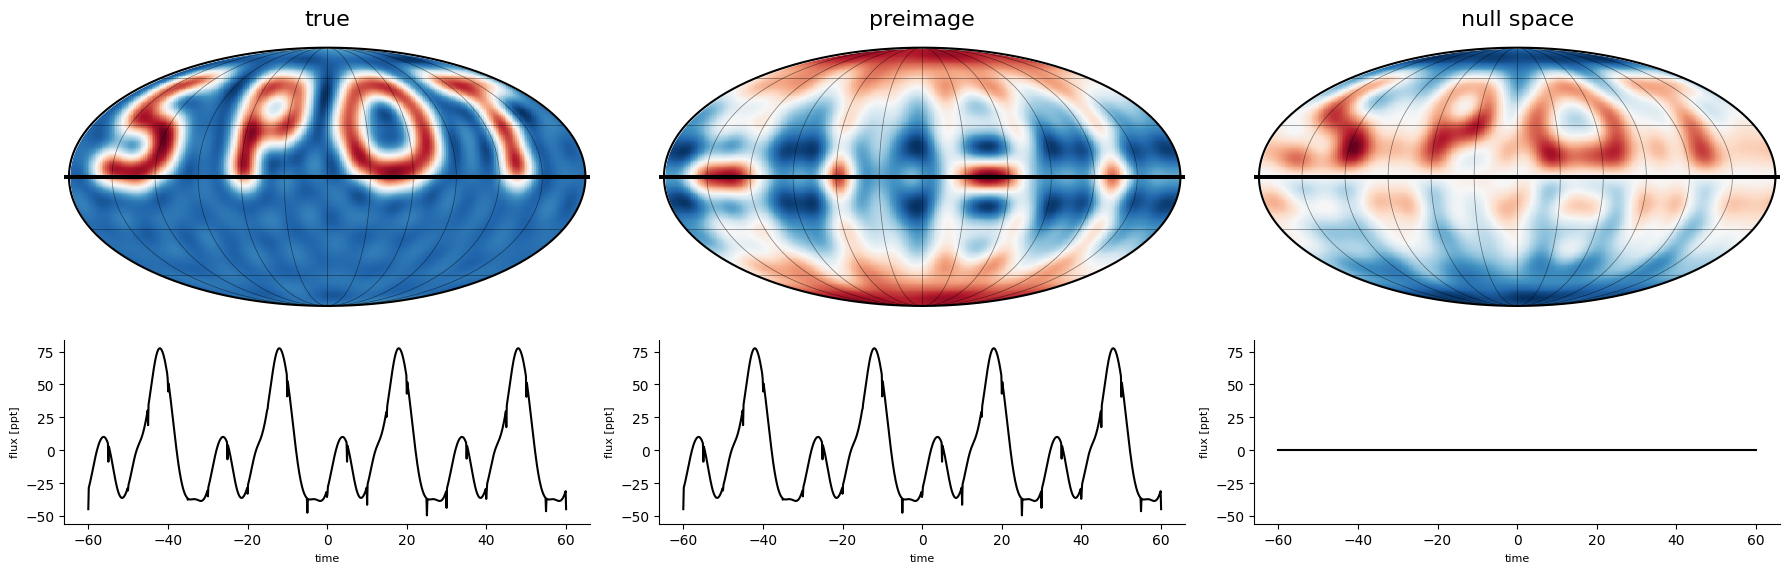
\includegraphics[width=\textwidth]{figures/nullspace-preimage.png}
        \caption{The breakdown of a surface map into its constituent components: the original map (left), its preimage (center), and null space (right). 
        Accompanying each set is the corresponding impact on the star's rotational light curve. The preimage represents surface patterns that 
        directly influence the observed light curve, while the null space encompasses patterns that have no effect on the flux measurements. 
        It's noteworthy that a significant portion of the surface features fall within the null space, meaning they do not contribute to the light curve 
        that we can observe and measure. The blck line shows the planetary trajectory, so what is important is that the preimage contains the full
        information under planetary trajectory, while the nullspace is missing it.}
        \label{fig:nullspace}
    \end{figure*}

%

\section{Hierarchical Bayesian model}
\label{sec:model}
In this section, we describe our Gaussian Process (GP) model and the likelihood calculation process used to estimate the model parameters.
This essentially means that we approximate the likelihood 
as a multidimensional Gaussian distribution characterized by a mean $\pmb{\mu}$ and covariance $\pmb{B}$ (for a comprehensive 
derivation of the Gaussian Process, refer to \cite{Luger2021b}):
%
\begin{align}
    \mathcal{L}\left(i_\star, P_\star, \mathbf{u}, \pmb{\theta}_\bullet\right) \sim
    \mathcal{N}\Big(
    \pmb{\mu}\left(i_\star, P_\star, \mathbf{u}, \pmb{\theta}_\bullet\right),
    \,
    \pmb{B}\left(i_\star, P_\star, \mathbf{u}, \pmb{\theta}_\bullet\right)
    \Big).
\end{align}
%
To infer the physical properties of the starposts, we want to obtain an underlying distribution of the physics conditioned on the provided data, 
which is known as the posterior distribution of the model.
% \subsection{Model for non-evolvng surfaces} \label{sec:nonevolmodel} 
We want to solve for a large set of parameters that includes the GP hyperparameters, the star's and the planet's orbital parameters, respectively. 
\begin{linenomath}\begin{align}
    \label{eq:largetheta}
    \pmb{\Theta}
     & =
    \left(
    \theta_\bullet
    \,\,\,
    \theta_\star
    \,\,\,
    \theta_p
    \right)^\top
    \quad,
\end{align}\end{linenomath}

Separately, these parameters are defined as 
\begin{linenomath}\begin{align}
    \label{eq:thetastar}
    \pmb{\theta_\star}
     & =
    \left(
    i_\star
    \,\,\,
    m_\star
    \,\,\,
    u_1
    \,\,\,
    u_2
    \,\,\,
    P_\star
    \right)^\top
    \quad,
\end{align}\end{linenomath}
where $i_\star$ is the star's orbital inclination, $m_\star$ is the stellar mass in the units of the solar mass, $u_1$ and $u_2$ are limb-darkening coefficients,
and $P_\star$ is the rotational period of the star.

\begin{linenomath}\begin{align}
    \label{eq:thetap}
    \pmb{\theta_p}
     & =
    \left(
    i_p
    \,\,\,
    e
    \,\,\,
    \lambda
    \,\,\,
    \omega
    \,\,\,
    P
    \,\,\,
    t_0
    \,\,\,
    R_p/R_\star
    \right)^\top
    \quad,
\end{align}\end{linenomath}
where $i_p$ is the planet's orbital inclination, $e$ is its eccenticity, $\lambda$ is the projected stellar obliquity, $\omega$ is the argument of pericenter of the planet,
$P$ is the rotational period of the planet, $t_0$ is the transit start time, and $R_p/R_\star$ is the planet to star radius ratio.

We represent the GP hyperparameters as \emph{physically interesting} set of parameters $\pmb{\theta}_\bullet$ \citep{Luger2021b}:
%
\begin{linenomath}\begin{align}
        \label{eq:thetaspot}
        \pmb{\theta}_\bullet
         & =
        \left(
        \mathbb{n}
        \,\,\,
        \mathbb{c}
        \,\,\,
        \sigma^2_\phi
        \,\,\,
        \mu_\phi
        \,\,\,
        \mathbb{r}
        \right)^\top
        \quad,
    \end{align}\end{linenomath}
%
where $\mathbb{n}$ is the number of starspots, $\mathbb{c}$ is their contrast (defined as the intensity difference between the spot and the 
background intensity, as a fraction of the background intensity), and $\mathbb{r}$ is the radius
of the spots, $\mu_\phi$ and $\sigma^2_\phi$ are the mean and variance of the latitude distribution. 
It could be more convenient to sample $\mu_\phi$ and $\sigma^2_\phi$ using $\mathbb{a}$ and $\mathbb{b}$, where
$\mathbb{a}$ and $\mathbb{b}$ are the normalized parameters of the Beta distribution in $\cos\phi$, which is the probability density function (PDF) 
for the latitude $\phi$ of the spots. These parameters have a one-to-one correspondence to the mode $\mu_\phi$ and standard deviation $\sigma_\phi$ of the 
distribution in $\phi$, allowing for a concise representation of the latitudinal distribution characteristics.
The Beta distribution in $\cos\phi$ which has hyperparameters $\alpha$ and $\beta$, and the PDF given by
%
\begin{align}
    \label{eq:cosphi-pdf}
    p \big(\cos\phi \, \big| \, \alpha, \beta \big)
     & =
    \dfrac{\Gamma(\alpha + \beta)}{\Gamma(\alpha)\Gamma(\beta)}
    (\cos\phi)^{\alpha - 1}
    (1 - \cos\phi)^{\beta - 1}
    \quad,
\end{align}
%
where $\Gamma$ is the Gamma function. The $\alpha$ and $\beta$ are derived from the normalized parameters 
%
\begin{align}
    \label{eq:beta2gauss}
    \alpha & = \exp\left({K_{00} + (\ln\frac{1}{2})\mathbb{a}}\right)
    \nonumber                                                 \\
    \beta  & = \exp\left({\ln\frac{1}{2} + (10 - \ln\frac{1}{2})\mathbb{b}}\right)
    \quad,
\end{align}
%
with inverse transform
%
\begin{align}
    \label{eq:gauss2beta}
    \mathbb{a} & \equiv \frac{\ln\alpha}{\ln\frac{1}{2}}
    \nonumber                                             \\[0.5em]
    \mathbb{b} & \equiv \frac{\ln\beta - \ln\frac{1}{2}}{10 -\ln\frac{1}{2}}
\end{align}
%
The parameters $\mathbb{a}$ and $\mathbb{b}$ are both constrained to values between 0 and 1, making them convenient for sampling during the inference process. 
However, $\mathbb{a}$ and $\mathbb{b}$ do not have a straightforward relationship with physically meaningful quantities. In many situations, it is preferable to parametrize 
the latitude distribution using two parameters: $\mu_\phi$, which controls the central latitude, and $\sigma_\phi$, which governs the dispersion of the 
spots' latitudes. Here, both the mean $\mu_\phi$ and variance $\sigma^2_\phi$ can be derived from the Beta distribution as
%
\begin{align}
    \label{eq:mean_beta}
    \mu_\phi
     & =
    \dfrac{\alpha}{\alpha+\beta}
    \quad,
\end{align}
%
\begin{align}
    \label{eq:var_beta}
    \sigma^2_\phi
     & =
    \dfrac{\alpha\beta}{(\alpha+\beta)^2(\alpha+\beta+1)}
    \quad,
\end{align}
%

We assume that the prior over $\mathbb{f}_{true}$ follows a multivariate Gaussian distribution, with a mean vector of zeros and a covariance 
matrix $\pmb{B}$. We use the quasi-periodic kernel to define the covariance matrix $\pmb{B}$, which is defined by \texttt{StarryProcess}.
We assume that the observations $\mathbb{f}_{obs}$ are corrupted by additive Gaussian noise, such that:
\begin{equation}
    \mathbb{f}_{obs} = \mathbb{f}_{true} + \epsilon
\end{equation}

where $\epsilon \sim \mathcal{N}(0, \sigma_n^2)$ is the noise term. Given the GP prior and the likelihood function, we can 
calculate the joint posterior distribution over the hyperparameters $\Theta$ and the true function $\mathbb{f}_{true}$ given the observed data $\mathbb{f}_{obs}$:
%
\begin{equation}
    p(\Theta, \mathbb{f}_{true} \mid \mathbb{f}_{obs}) \propto p(\Theta) p(\mathbb{f}_{true} \mid \Theta) p(\mathbb{f}_{obs} \mid \mathbb{f}_{true})
\end{equation}
%
where $P(\Theta)$ is the prior distribution over the hyperparameters, $P(\mathbb{f}_{true} \mid \Theta)$ is the likelihood of the true function given 
the hyperparameters, and $P(f_{obs} \mid f_{true})$ is the likelihood of the observed data given the true function.
We calculate the log-likelihood function, given by (\citep{Luger2021b}):
%
% \begin{linenomath}\begin{align}
%     \label{eq:log-likeSabina}
%     \ln p(\mathbb{f}_{obs} \mid \pmb{\Theta}) 
%     =
%     & -\frac{1}{2} (\mathbb{f}_{obs} - \pmb{\mu})^T \pmb{B}^{-1} (\mathbb{f}_{obs} - \pmb{\mu}) 
%     \nonumber       \\[0.75em]
%     & -
%     \frac{1}{2} \ln |\pmb{B}| - \frac{n}{2} \ln (2\pi)
%     \quad,
% \end{align}\end{linenomath}
% %
% or, as defined in eq. 14 of \citep{Luger2021b}:
%
\begin{linenomath}\begin{align}
    \label{eq:log-likeRodrigo}
    \ln \mathcal{L}_m\left(\Theta\right)
    =
     & -\frac{1}{2}
    \mathbf{r}_m^\top\left(\Theta\right)
    \big[
        \pmb{B}\left(\Theta\right)
        \big]^{-1}
    \mathbf{r}_m\left(\Theta\right)
    \nonumber       \\[0.75em]
     & -
    \frac{1}{2}
    \ln \Big|
    \pmb{B}\left(\Theta\right)
    \Big|
    -
    \frac{K}{2}
    \ln \left( 2 \pi \right)
    \quad,
\end{align}\end{linenomath}
%
where
%
\begin{linenomath}\begin{align}
        \mathbf{r}_m\left(\pmb{\Theta}\right)
         & \equiv
        \mathbf{f}_m - \pmb{\mu}\left(\pmb{\Theta}\right)
    \end{align}\end{linenomath}
%
is defined as the residual vector,
%
$\pmb{B}$ is the full covariance, which is defined as 
%
\begin{linenomath}\begin{align}
    \pmb{B}\left(\Theta\right)
     & \equiv
    \pmb{\Lambda} + \pmb{C}
\end{align}\end{linenomath}
%
where $\pmb{\Lambda}$ is the covariance of the distribution over spherical harmonic coefficient
vectors $\mathbb{y}$, and $\pmb{C}$ is the data covariance, which is a diagonal
matrix whose entries are the squared uncertainty $\sigma_m^2$ corresponding to each data point in the light curve.
$| \cdots |$ denotes the determinant, and $K$ is the number of data points in
each light curve.%

For faster calculations we rewrite the likelihood function using \emph{the matrix conversion lemma}, also known as 
Woodbury-Sherman-Morrison identity \citep[see, e.g.,][]{Hogg2020}, which gives an expression for the inverse $\pmb{B}^{-1}$ of the marginalized likelihood variance:
%
\begin{linenomath}\begin{align}
    \label{eq:Hoggtrick}
    \pmb{B}^{-1} = \pmb{C}^{-1} - \pmb{C}^{-1} \pmb{M} (\pmb{\mathbb{I}} 
    & + \pmb{\Lambda} \pmb{M}^T \pmb{C}^{-1}\pmb{M})^{-1}\pmb{\Lambda} \pmb{M}^T\pmb{C}^{-1}
\end{align}\end{linenomath}
%

% \section{Experiments}
% In this section, we describe the experiments we did on synthetic light curves before going ahead and modeling the real data. The synthetic light curves were 
% generated by initializing a planet and a star of similar parameters as HAT-P-11 b and HAT-P-11 have using \texttt{starry}. Then we draw \texttt{StarryProcess} 
% samples from a prior to get spherical harmonic coefficients and consequently the simulated flux. 

\subsection{The issue of the normalization of light curves and units}
Before going on discussing the experiments produced for this paper, we first need to remind the reader of a subtlety of the flux normalization when we are given
the raw light curves from telescopes. The problem and the ways to tackle it were described in \cite{Luger2021a} and \cite{Luger2021b}. 

Briefly, the problem of normalization of light curves is related to the fact that the observed flux from a star can vary due to a variety of factors 
such as atmospheric effects, instrumental noise, and changes in the intrinsic brightness of the star itself. These variations can make it difficult 
to compare light curves of different stars or even the same star observed at different times. To address this problem, astronomers typically normalize 
light curves by dividing the observed flux by some factor (the median or mean of the flux) that is assumed to be constant over time. 
However, as was described in \cite{Luger2021a}, if a star has a single large equatorial spot of contrast $c$ viewed at some high inclination 
(\cite{Luger2021a} used the value of $60^o$), and another star with a spot at the same location but with half the contrast \emph{and} a large polar spot of 
comparable contrast, then the light curves for both of the stars become indistiguishable in the relative units astronomers observe them. In addition to normalizing 
the flux, \cite{Luger2021a} also added a \emph{baseline} (1 in their case), which is the flux one would have gotten from a spotless star, 
and is an additive component to the $Y_m^l$.

In our experiments, we noticed that dividing by a constant factor \emph{and} adding an additive baseline messes up the units due to the 
intricate transition between the spherical harmonics and flux unit bases. To address this issue, we opt for an alternative approach, wherein we 
impose a constraint upon the constant terms within the map, which correspond to a featureless star. Specifically, we achieve this by setting the prior distribution 
over these constant terms to be entirely uniform, thereby setting the first row of the precision matrix to zero, which is us telling the model that
\textit{we don't know what the baseline is}.

Let $\mathbf{K}$ be the precision matrix, which is the inverse of the covariance matrix $\mathbf{B}$. Then the precision matrix looks as
%
\begin{linenomath}\begin{align}
    \mathbf{K} = 
    \begin{bmatrix}
    0 & 0 & \cdots & 0 \\
    0 & k_{22} & \cdots & k_{2n} \\
    \vdots & \vdots & \ddots & \vdots \\
    0 & k_{n2} & \cdots & k_{nn}
    \end{bmatrix}
\end{align}\end{linenomath}
%
where $k_{ij}$ represents the elements of the precision matrix $\mathbf{K}$.

By setting the first row of the precision matrix to zero, we effectively impose a uniform prior distribution over the constant terms in the map, thereby 
addressing the issue of unit mismatch caused by dividing by a constant factor and adding an additive baseline.

% In our experiments, we noticed that dividing by a constant factor \emph{and} adding an additive baseline messes up the units due to the complex change of 
% basis from spherical harmonics to the flux units. Instead, in our model, we set the baseline, i.e the first column of the design matrix, $\pmb{\mathcal{A}}$, 
% to have the coefficients of the 0th harmonic, $Y^0_0$ -- the featureless star. Then, the normalization "factor" becomes additive (not multiplicative!). We're reminding 
% the reader that $\pmb{\mathcal{A}}$ covers the properties of the star and the planet (inclination, rotation period, transit, etc.), spherical harmonics desribe the
% properties of the starspots. Therefore, what we get is
% %
% \begin{linenomath}\begin{align}
%         \label{eq:fAy}
%         \mathbf{f} = \pmb{\mathcal{a}_0(t)} \mathbf{y_0(t)} + \sum_{l=1, m=-l}^{15} \pmb{\mathcal{a}_{lm}(t)} \mathbf{y_{lm}(t)},
%     \end{align}\end{linenomath}
% %
% where $\pmb{\mathcal{a}_0}$ is a column of $\pmb{\mathcal{A}}(I, P, \mathbf{u})$, which is the design matrix as a function of the stellar inclination, rotation period, 
% and limb-darkening coefficients; $\mathbf{y}$ is a spherical harmonic coefficient vector, and we define $\pmb{\mathcal{a}_0} \mathbf{y_0} = \pmb{m}$ 
% as the normalization constant, or a \emph{baseline}. We explicitly solve for the baseline in our model. Note that it is not constant with time due to the transits --
% $\pmb{m}$ drops when the planet is transitting the star.

\subsection{Stellar inclination and obliquity}
\label{sec:obl-inc}
In the Sectrion \ref{sec:results-synthetic}, we hope to convince the reader that there is a a good amount of information about stars that we can learn 
from disk-integrated photometric measurements. In particular, Figure \ref{fig:inclination} illustrates the profound impact of stellar inclination on observed light curves. 
As the inclination angle varies from pole-on ($0^\circ$) to equator-on ($90^\circ$) views, we observe significant changes in both the amplitude and 
morphology of the light curve modulations. At low inclinations, when we view the star more pole-on, the light curves exhibit smaller amplitude variations. 
This is because the spots remain invisible throughout the stellar rotation, leading to more subtle flux changes. As the inclination increases towards an 
equator-on perspective, the amplitude of the variations typically increases, and the shape of the light curve becomes more pronounced. These changes occur because 
at higher inclinations, spots periodically disappear from view as the star rotates, causing more dramatic swings in the observed flux. 
The effect is particularly noticeable for spots at mid-latitudes, which can produce sharp dips in the light curve as they rotate into and out of view. 
It's important to note that while inclination significantly affects the observed light curve, it does not alter the underlying rotation period of 
the star or the intrinsic properties of the spots themselves.

While variations in stellar obliquity can have significant implications for planetary systems, their effects on the overall stellar light curve 
are often not noticeable. The global light curve is primarily influenced by the star's rotation and the distribution of spots on its surface, 
with obliquity playing a less prominent role. However, the impact of stellar obliquity becomes much more apparent during planetary transits, 
particularly through the phenomenon of spot-crossing events. When a planet transits its host star, it can occult starspots along its path. 
These spot-crossing events manifest as brief increases in brightness during the transit, as the planet temporarily blocks a darker region of the stellar 
surface. The frequency, timing, and duration of these spot-crossing events are strongly influenced by the alignment between the stellar spin axis and 
the planet's orbital plane - in other words, the stellar obliquity. Figure \ref{fig:obliquity} shows three consecutive transit light curves for 
different stellar obliquities. Each row in the figure represents a different obliquity scenario, with obliquity increasing from left to right. 
The rows display three consecutive transits for each scenario. 
In systems with low obliquity, where the stellar equator is aligned with the 
planet's orbit, spot-crossing events tend to occur more regularly and predictably. This is evident in the first column of Figure \ref{fig:obliquity}, where the spot-crossing patterns show a more consistent appearance across consecutive transits. 
Conversely, in systems with high obliquity, the pattern of spot-crossings can be more erratic and less frequent. This is because the planet's transit path across 
the stellar disk intersects a different range of stellar latitudes, potentially missing spots concentrated at certain latitudes. The $90^\circ$ column of 
Figure \ref{fig:obliquity} demonstrates this, showing more varied and less predictable spot-crossing patterns between consecutive transits. 
Therefore, while the full-disk light curve may not clearly reveal changes in stellar obliquity, careful analysis of in-transit light curves, 
particularly focusing on spot-crossing events, can provide valuable insights into the star's orientation relative to the planetary orbit. 

\begin{figure*}[hbt!]
    % \script{experiment-1-true-map.py}
    \begin{centering}
        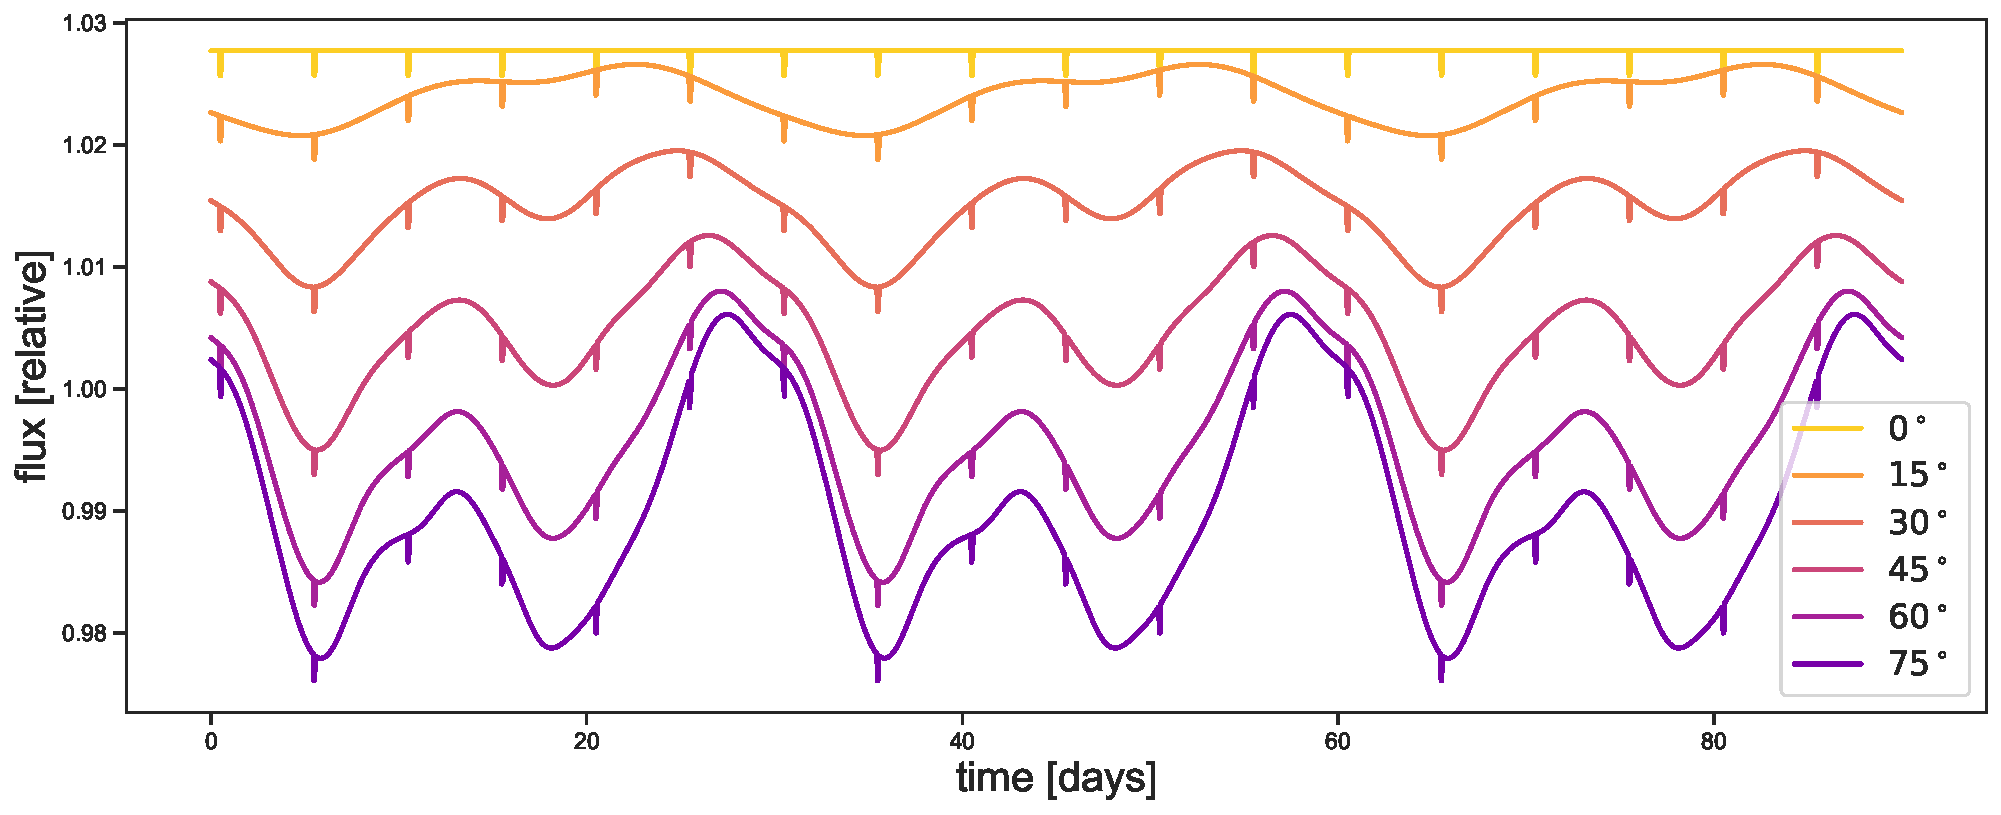
\includegraphics[width=\linewidth]{figures/inclinations.pdf}
        \caption{
            Variation in stellar light curves as a function of inclination angle. Each curve displays the photometric time series (light curve) for a 
            hypothetical spotted star observed at different inclination angles. The x-axis represents time in days, while the y-axis shows the relative flux. 
            Inclination angles range from $0^\circ$ (pole-on view) to $90^\circ$ (equator-on view). Note how the amplitude and shape of the light 
            curve modulations change significantly with inclination, demonstrating the importance of this parameter in interpreting stellar variability. 
            The star's rotation period and spot configuration remain constant across all light curves.
        }
        \label{fig:inclination}
    \end{centering}
\end{figure*}

\begin{figure*}[hbt!]
    % \script{experiment-1-true-map.py}
    \begin{centering}
        \includegraphics[width=\linewidth]{figures/obliquities.pdf}
        \caption{
            Impact of stellar obliquity on consecutive planetary transit light curves. Each column represents a different stellar obliquity scenario, 
            with obliquity increasing from left to right. The rows show three consecutive transits for each scenario. The x-axis represents time relative to 
            the transit center, while the y-axis shows the normalized flux. Note the varying patterns of in-transit brightness fluctuations 
            (spot-crossing events) across different obliquities and between consecutive transits. These differences arise from the changing 
            geometry between the planet's transit path and the distribution of starspots at different stellar latitudes. 
            The consistent transit depth and duration across all panels indicate that other system parameters remain constant, 
            isolating the effect of stellar obliquity.
        }
        \label{fig:obliquity}
    \end{centering}
\end{figure*}


While the analysis of spot-crossing events in transit light curves provides a powerful tool for constraining stellar inclination and obliquity, 
there exists an important degeneracy in these measurements. Specifically, a system with stellar inclination $i_\star$ and obliquity $-\lambda_\star$ 
will produce identical light curves to a system with inclination $180-i_\star$ and obliquity $\lambda_\star$, but with a surface map flipped upside down.

This degeneracy arises from the symmetry in the geometry of the star-planet system. In both scenarios, the relative orientation between the stellar 
rotation axis and the planet's orbital plane remains the same, merely mirrored. As a result, the pattern of spot crossings and their evolution over 
multiple transits will be indistinguishable between these two configurations.

For example, a star with an inclination of $80^\circ$ and an obliquity of $-30^\circ$ will present the same transit light curves 
as a star with an inclination of $100^\circ$ and an obliquity of $30^\circ$ with a flipped map (see Figure \ref{fig:inc-obliquity-degeneracy}). 
In both cases, the angle between the stellar spin axis and the planet's orbital axis is identical, just reflected about the plane of the sky.
This degeneracy highlights a limitation in our ability to uniquely determine stellar geometry solely from transit light curve analysis. 
While we can constrain the relative alignment between the stellar spin and planetary orbit with high precision, we cannot distinguish between these 
mirrored configurations without additional information or observations.


\begin{figure}[hbt!]
    % \script{experiment-1-true-map.py}
    \begin{centering}
        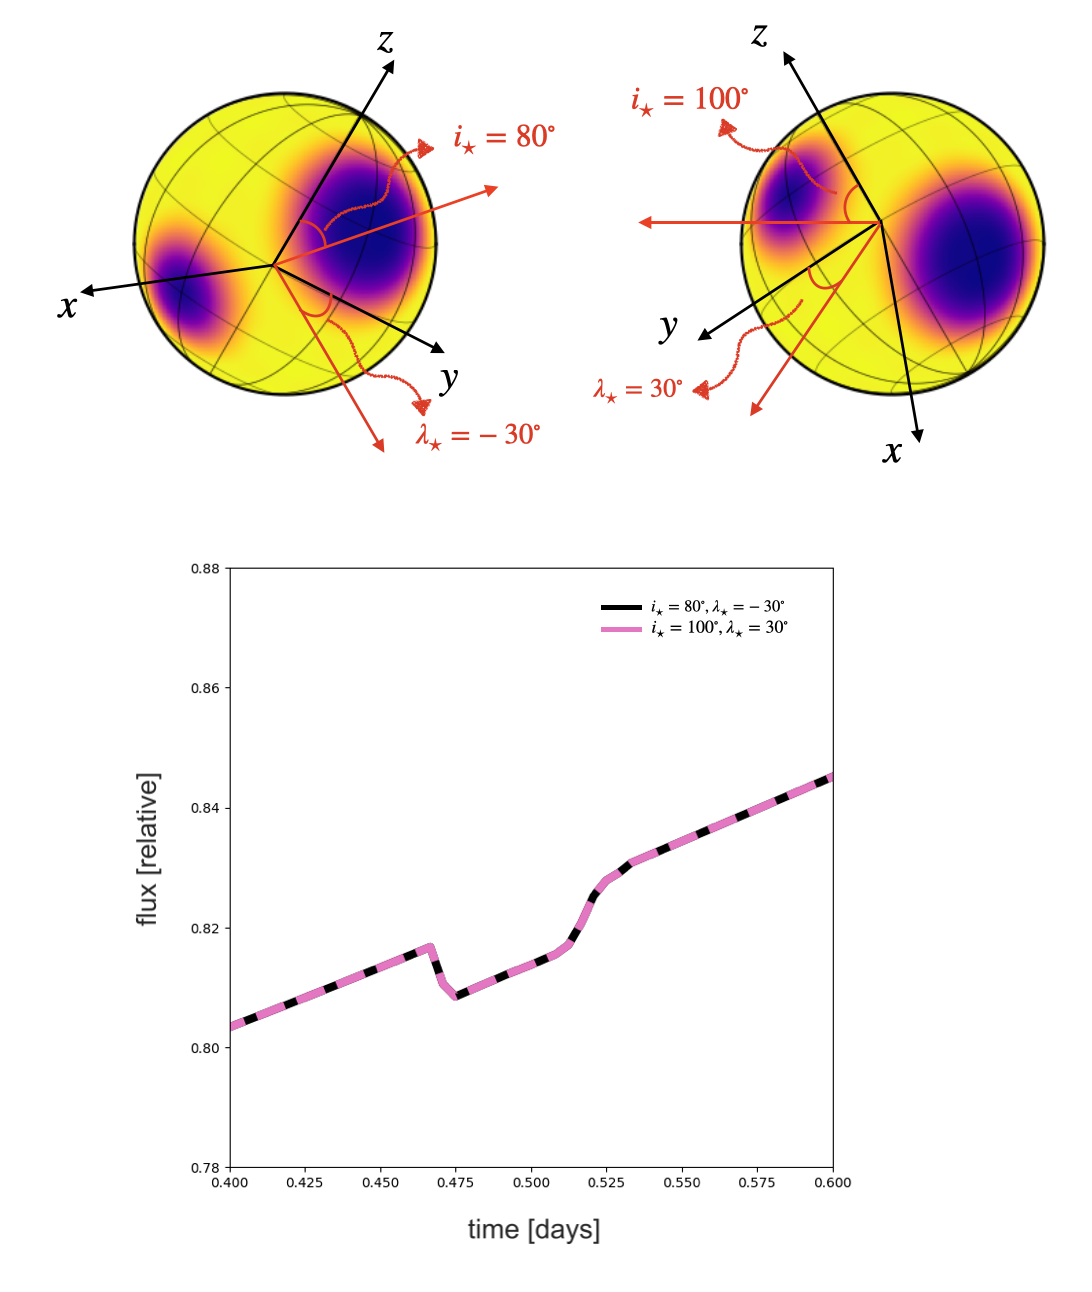
\includegraphics[width=\linewidth]{figures/inc-obl-degeneracy.png}
        \caption{
            Illustration of the degeneracy between stellar inclination ($i_\star$) and obliquity ($\lambda_\star$) in transit light curves. 
            The left panel shows a star-planet system with inclination $i_\star$ and obliquity $-\lambda_\star$, while the right panel 
            depicts a system with inclination $180-i_\star$ and obliquity $\lambda_\star$ and with a flipped map. 
            Despite the different geometries, both configurations result in identical transit light curves, shown in the central plot. 
            The x-axis represents time relative to the transit center, and the y-axis shows normalized flux. 
            This degeneracy demonstrates that while transit light curves can constrain the relative alignment between stellar spin and planetary orbit, 
            they cannot distinguish between these mirrored configurations without additional information. 
            The angles are represented with $x$, $y$, and $z$ vectors.
        }
        \label{fig:inc-obliquity-degeneracy}
    \end{centering}
\end{figure}

Given the degeneracy between stellar inclination and obliquity, a naive sampling approach could lead to unnecessary computational costs and potential 
convergence issues. To address this, we can leverage the fact that inclination and obliquity can be represented as vectors in three-dimensional 
space (see Figure \ref{fig:inc-obliquity-degeneracy}). This allows us to implement a more efficient sampling strategy that breaks the degeneracy 
while maintaining physical consistency.

We introduce transformed variables $\tilde{x}$, $\tilde{y}$, and $\tilde{z}$, on which we place prior distributions. 
Specifically, we use normal priors for $\tilde{x}$ and $\tilde{y}$, and a half-normal prior for $\tilde{z}$ to ensure it remains positive. 
These priors are chosen to explore the parameter space effectively while respecting physical constraints.

The transformation from these sampled variables to the physical space is then defined as:
\begin{linenomath}\begin{align}
    \label{eq:xyz}
    x = \tilde{x}, \\ 
    y = \frac{\sqrt{2}}{2} (\tilde{z} + \tilde{y}), \\
    z = \frac{\sqrt{2}}{2} (\tilde{z} - \tilde{y})
\end{align}\end{linenomath}

From these transformed coordinates, we can derive the stellar inclination and obliquity:

\begin{linenomath}\begin{align}
    \label{eq:obl-inc}
    i_\star = \arctan{\frac{y}{x}}, \\ 
    \lambda_\star = \arccos{\frac{z}{\sqrt{x^2 + y^2 + z^2}}}
\end{align}\end{linenomath}

This approach effectively breaks the degeneracy during the sampling process. By sampling in this transformed space and then mapping back to 
the physical parameters, we ensure that our model explores the full range of physically meaningful configurations without redundancy. 
This not only improves the efficiency of our sampling but also provides unambiguous constraints on the stellar geometry.

% \subsection{Step-by-step model instruction}
% In this section, we provide a comprehensive, step-by-step description of our model's methodology. 
% This process outlines the key stages in our analysis, from initial data preparation to the final likelihood computation:

% \begin{enumerate}
%     \item Acquire the target system's light curve data.
%     \item Preprocess the data by binning the out-of-transit observations to optimize computational efficiency while preserving signal fidelity.
%     \item Construct a design matrix incorporating both planetary (transit) and stellar orbital parameters, encapsulating the geometry of the star-planet system.
%     \item Establish physically motivated hyperparameters and prior distributions based on current astrophysical understanding and observational constraints.
%     \item Implement a sampling algorithm to draw from the defined prior distributions, exploring the parameter space efficiently.
%     % \item Generate synthetic light curves from the sampled parameters, simulating the observed stellar and planetary signals.
%     \item Compute the covariance matrix for the Gaussian process, which models the stochastic components of stellar variability.
%     \item Assemble the inverse of the full covariance matrix, combining deterministic and stochastic elements of the model based on Equation \ref{eq:Hoggtrick}.
%     \item Calculate the likelihood of the observed data given the model parameters, quantifying the agreement between our model and the observations with Equation \ref{eq:log-likeRodrigo}.
% \end{enumerate}

\subsection{Model for evolving surfaces}
\label{sec:evolmodel}
Some active stars, particularly Sun-like stars, exhibit surface evolution on timescales as short as a single rotation period. For example, starspots can appear and dissipate within days or weeks, 
while chromospheric plages and coronal loops can flare up and decay on even shorter timescales. Such rapid evolution of surface structures violates 
the fundamental assumption of a static photosphere underlying the model described in Section \ref{sec:model}. 
Accounting for these time-dependent surface phenomena is crucial for accurately interpreting observations of active stars, as they can introduce significant 
time-varying distortions in the photometric light curves. 

Here, we describe an improved model that accounts for the surface evolution.

To account for the time-varying nature of the stellar surface maps, we have extended the model described in Section \ref{sec:model} to allow 
for a smooth evolution of the maps over time. We assume that the surface map transitions smoothly from one epoch to the next, with the spherical harmonic 
coefficients linearly interpolated between consecutive map epochs. 

Specifically, let $\pmb{y}_1$, $\pmb{y}_2$, $\pmb{y}_3$, ... represent the spherical harmonic coefficient vectors describing the surface maps at a 
sequence of epochs $\pmb{t}_1$, $\pmb{t}_2$, $\pmb{t}_3$, ... For any time $\pmb{t}$ between two consecutive epochs $\pmb{t}_i$ and $\pmb{t}_{i+1}$, 
the coefficient vector $\pmb{y(t)}$ is obtained by linear interpolation:
\begin{linenomath}\begin{align}\label{linearinterp}
    \pmb{y(t)} = (1 - \alpha)\pmb{y}_i + \alpha\pmb{y}_{i+1},
\end{align}\end{linenomath}

where $\alpha = (\pmb{t} - \pmb{t}_i) / (\pmb{t}_{i+1} - \pmb{t}_i)$ is the linear interpolation factor between the epochs. 
This interpolation scheme ensures the surface map smoothly deforms from $\pmb{y}_i$ at time $\pmb{t}_i$ to $\pmb{y}_{i+1}$ at the next epoch $\pmb{t}_{i+1}$.

A key aspect is that each pair of consecutive maps $\pmb{y}_i$, $\pmb{y}_{i+1}$ is interpolated independently from other map pairs. 
Thus, $\pmb{y}_{i+1}$ does not depend on $\pmb{y}_{i-1}$, and $\pmb{y}_{i+2}$ is independent of $\pmb{y}_{i+1}$, allowing the model greater 
flexibility to fit arbitrary time variations. The framework developed for static maps in Section \ref{sec:model} is applied independently 
to each interpolated map $\pmb{y(t)}$, with the transition between maps governed by the linear interpolation above.

% \subsection{Experiment on a non-evolving star}
% For our initial experiment with minimal complexity, we created a synthetic light curve that involved a single planetary transit (therefore, 
% \emph{a short light curve}). Here, we examined two distinct sampling techniques: No-U-Turn Sampling (NUTS) using \texttt{pymc3} and Markov Chain Monte Carlo (MCMC) 
% using \texttt{emcee}. The MCMC technique exhibited a faster convergence rate of the walkers, despite the fact that it still required a significant amount of time.
% \subsection{Long light curves (multiple transits)}

% \begin{figure}[ht!]
%     \script{synthetic_data.py}
%     \begin{centering}
%         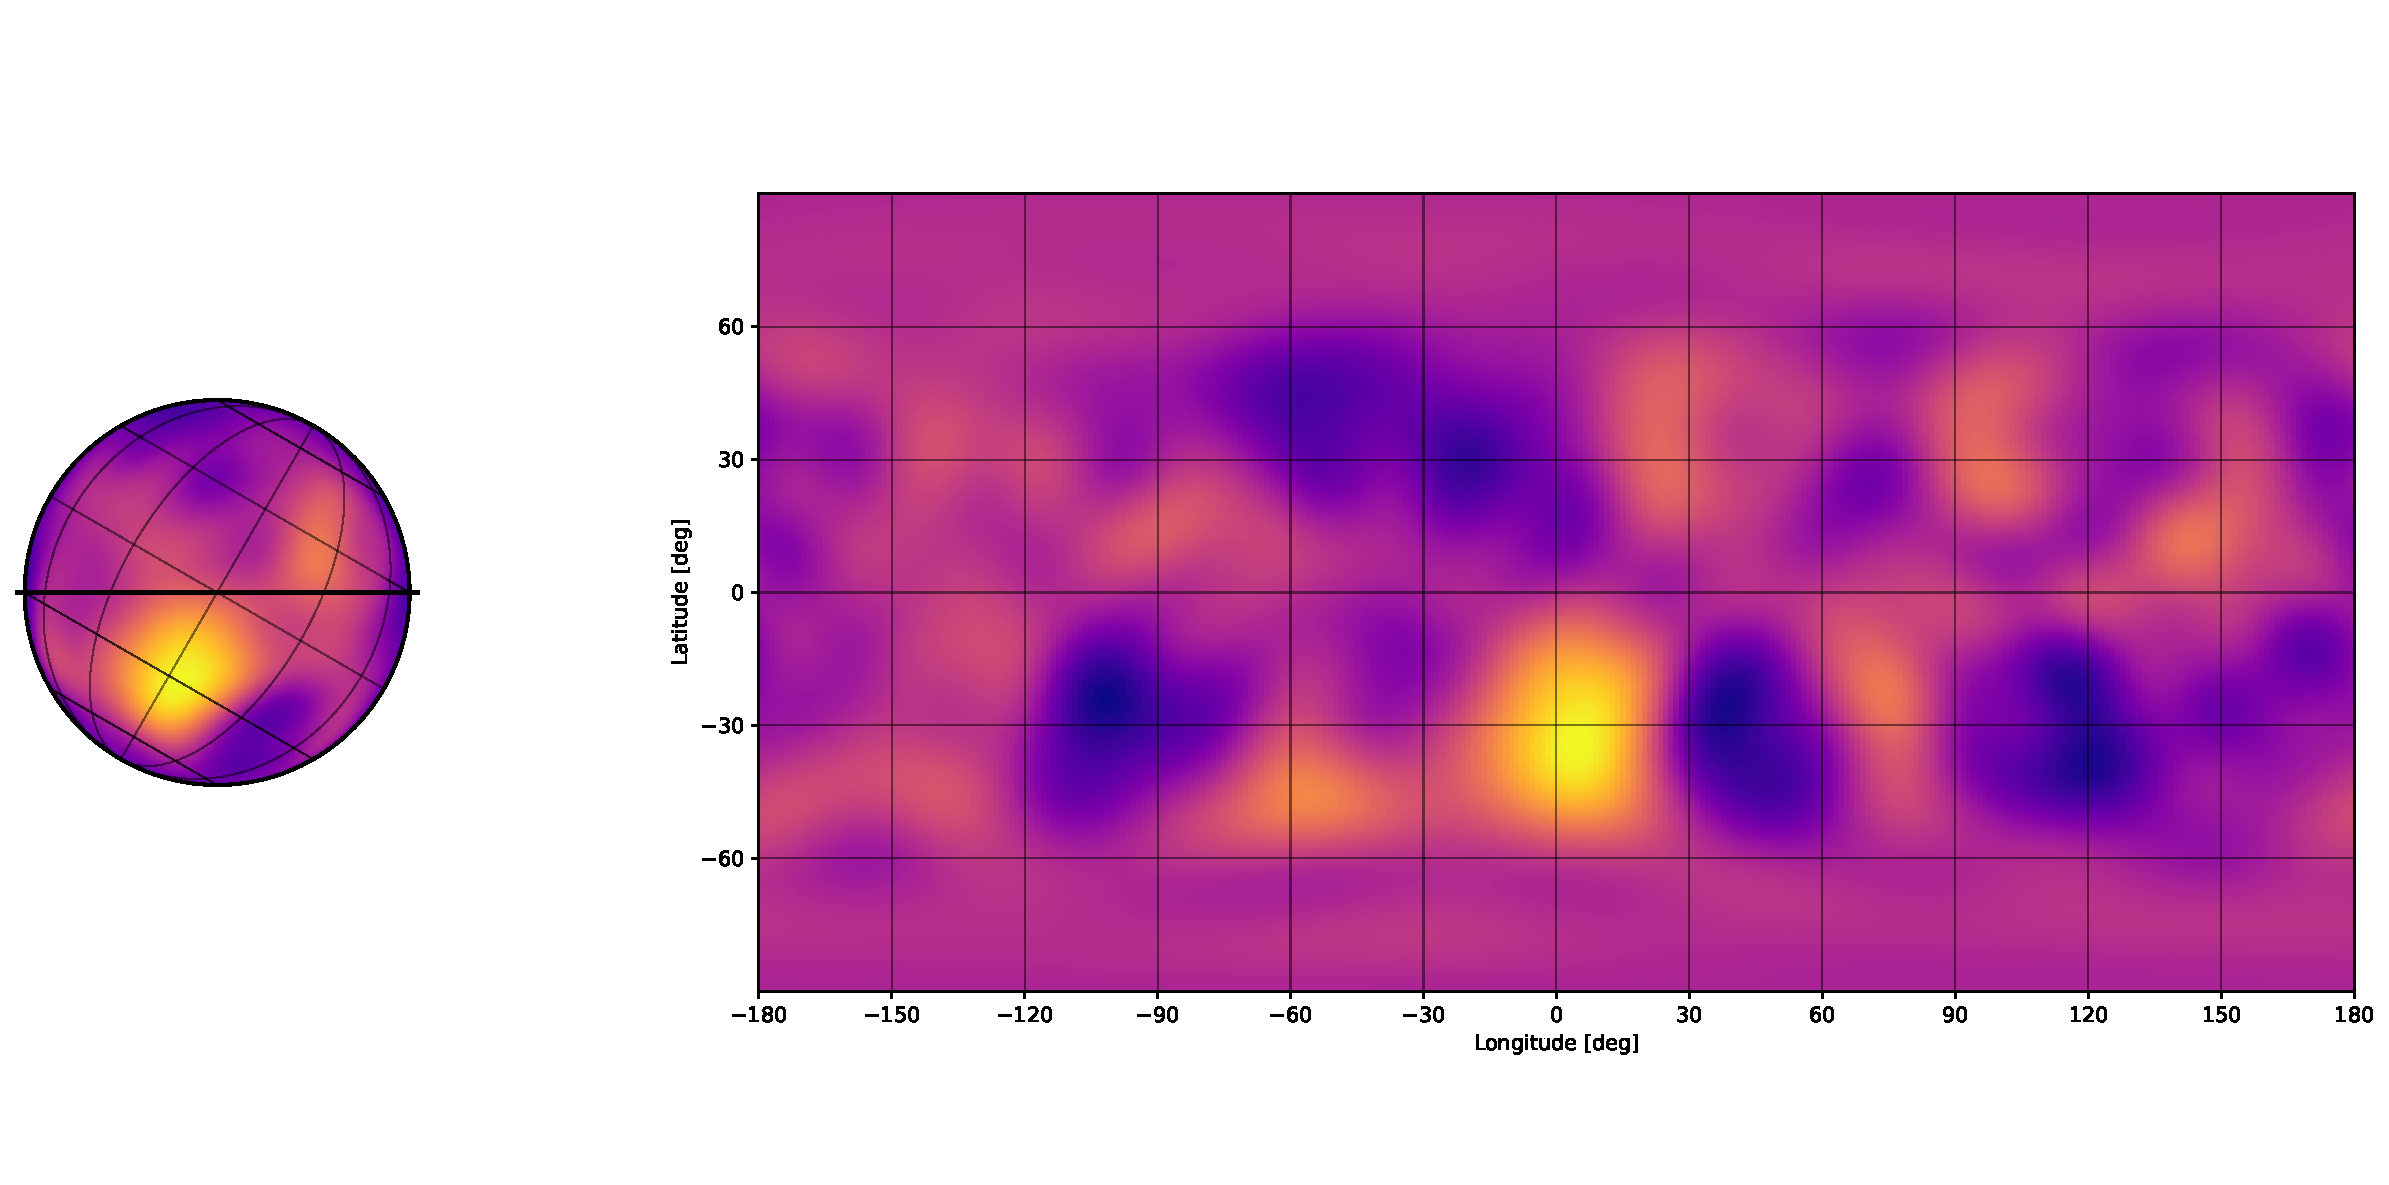
\includegraphics[width=\linewidth]{figures/SyntheticDataMap.pdf}
%         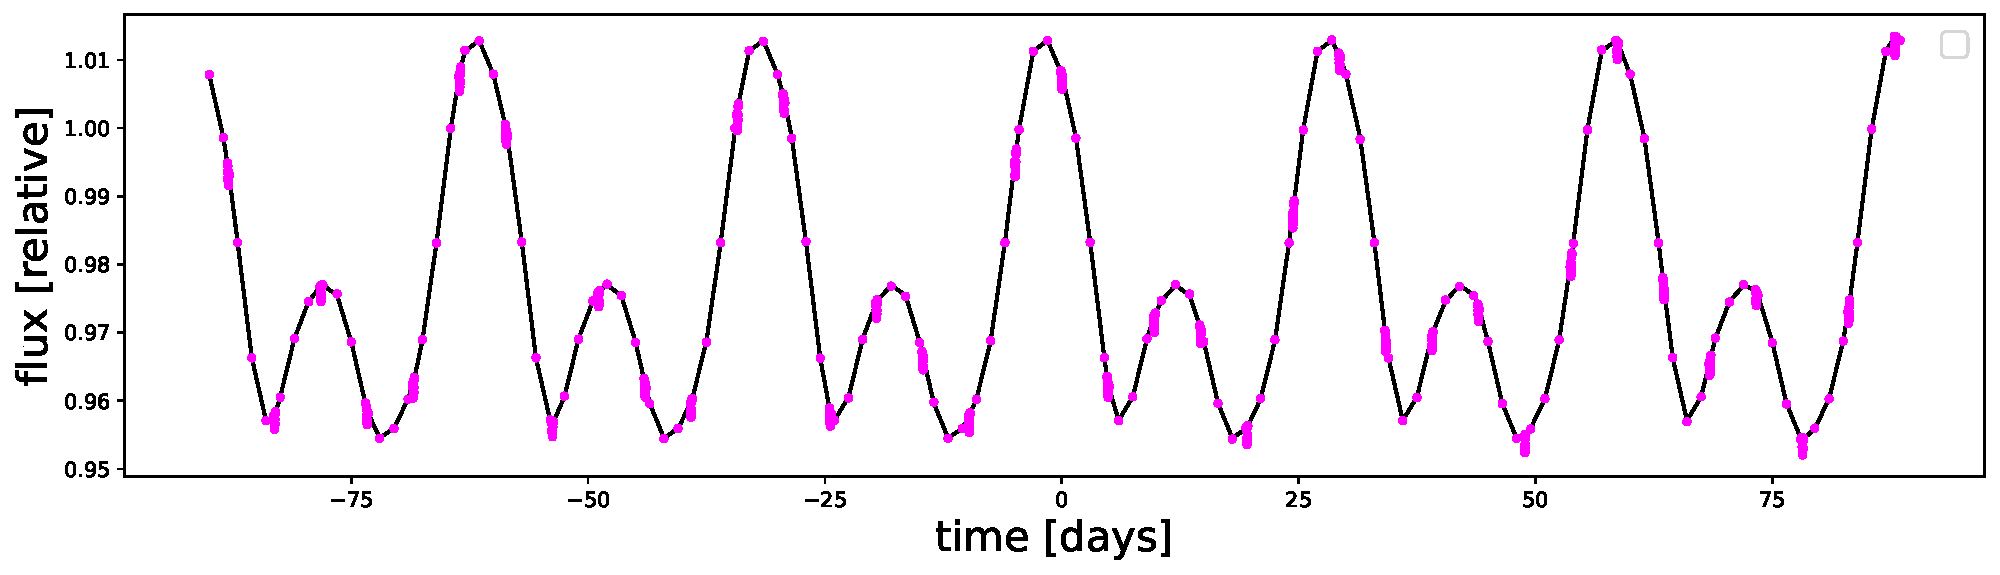
\includegraphics[width=\linewidth]{figures/SyntheticDataLightCurve.pdf}
%         \caption{
%             A synthetic dataset.
%         }
%         \label{fig:SyntheticDataLc}
%     \end{centering}
% \end{figure}

% \begin{figure}[ht!]
%     \script{synthetic_data.py}
%     \begin{centering}
%         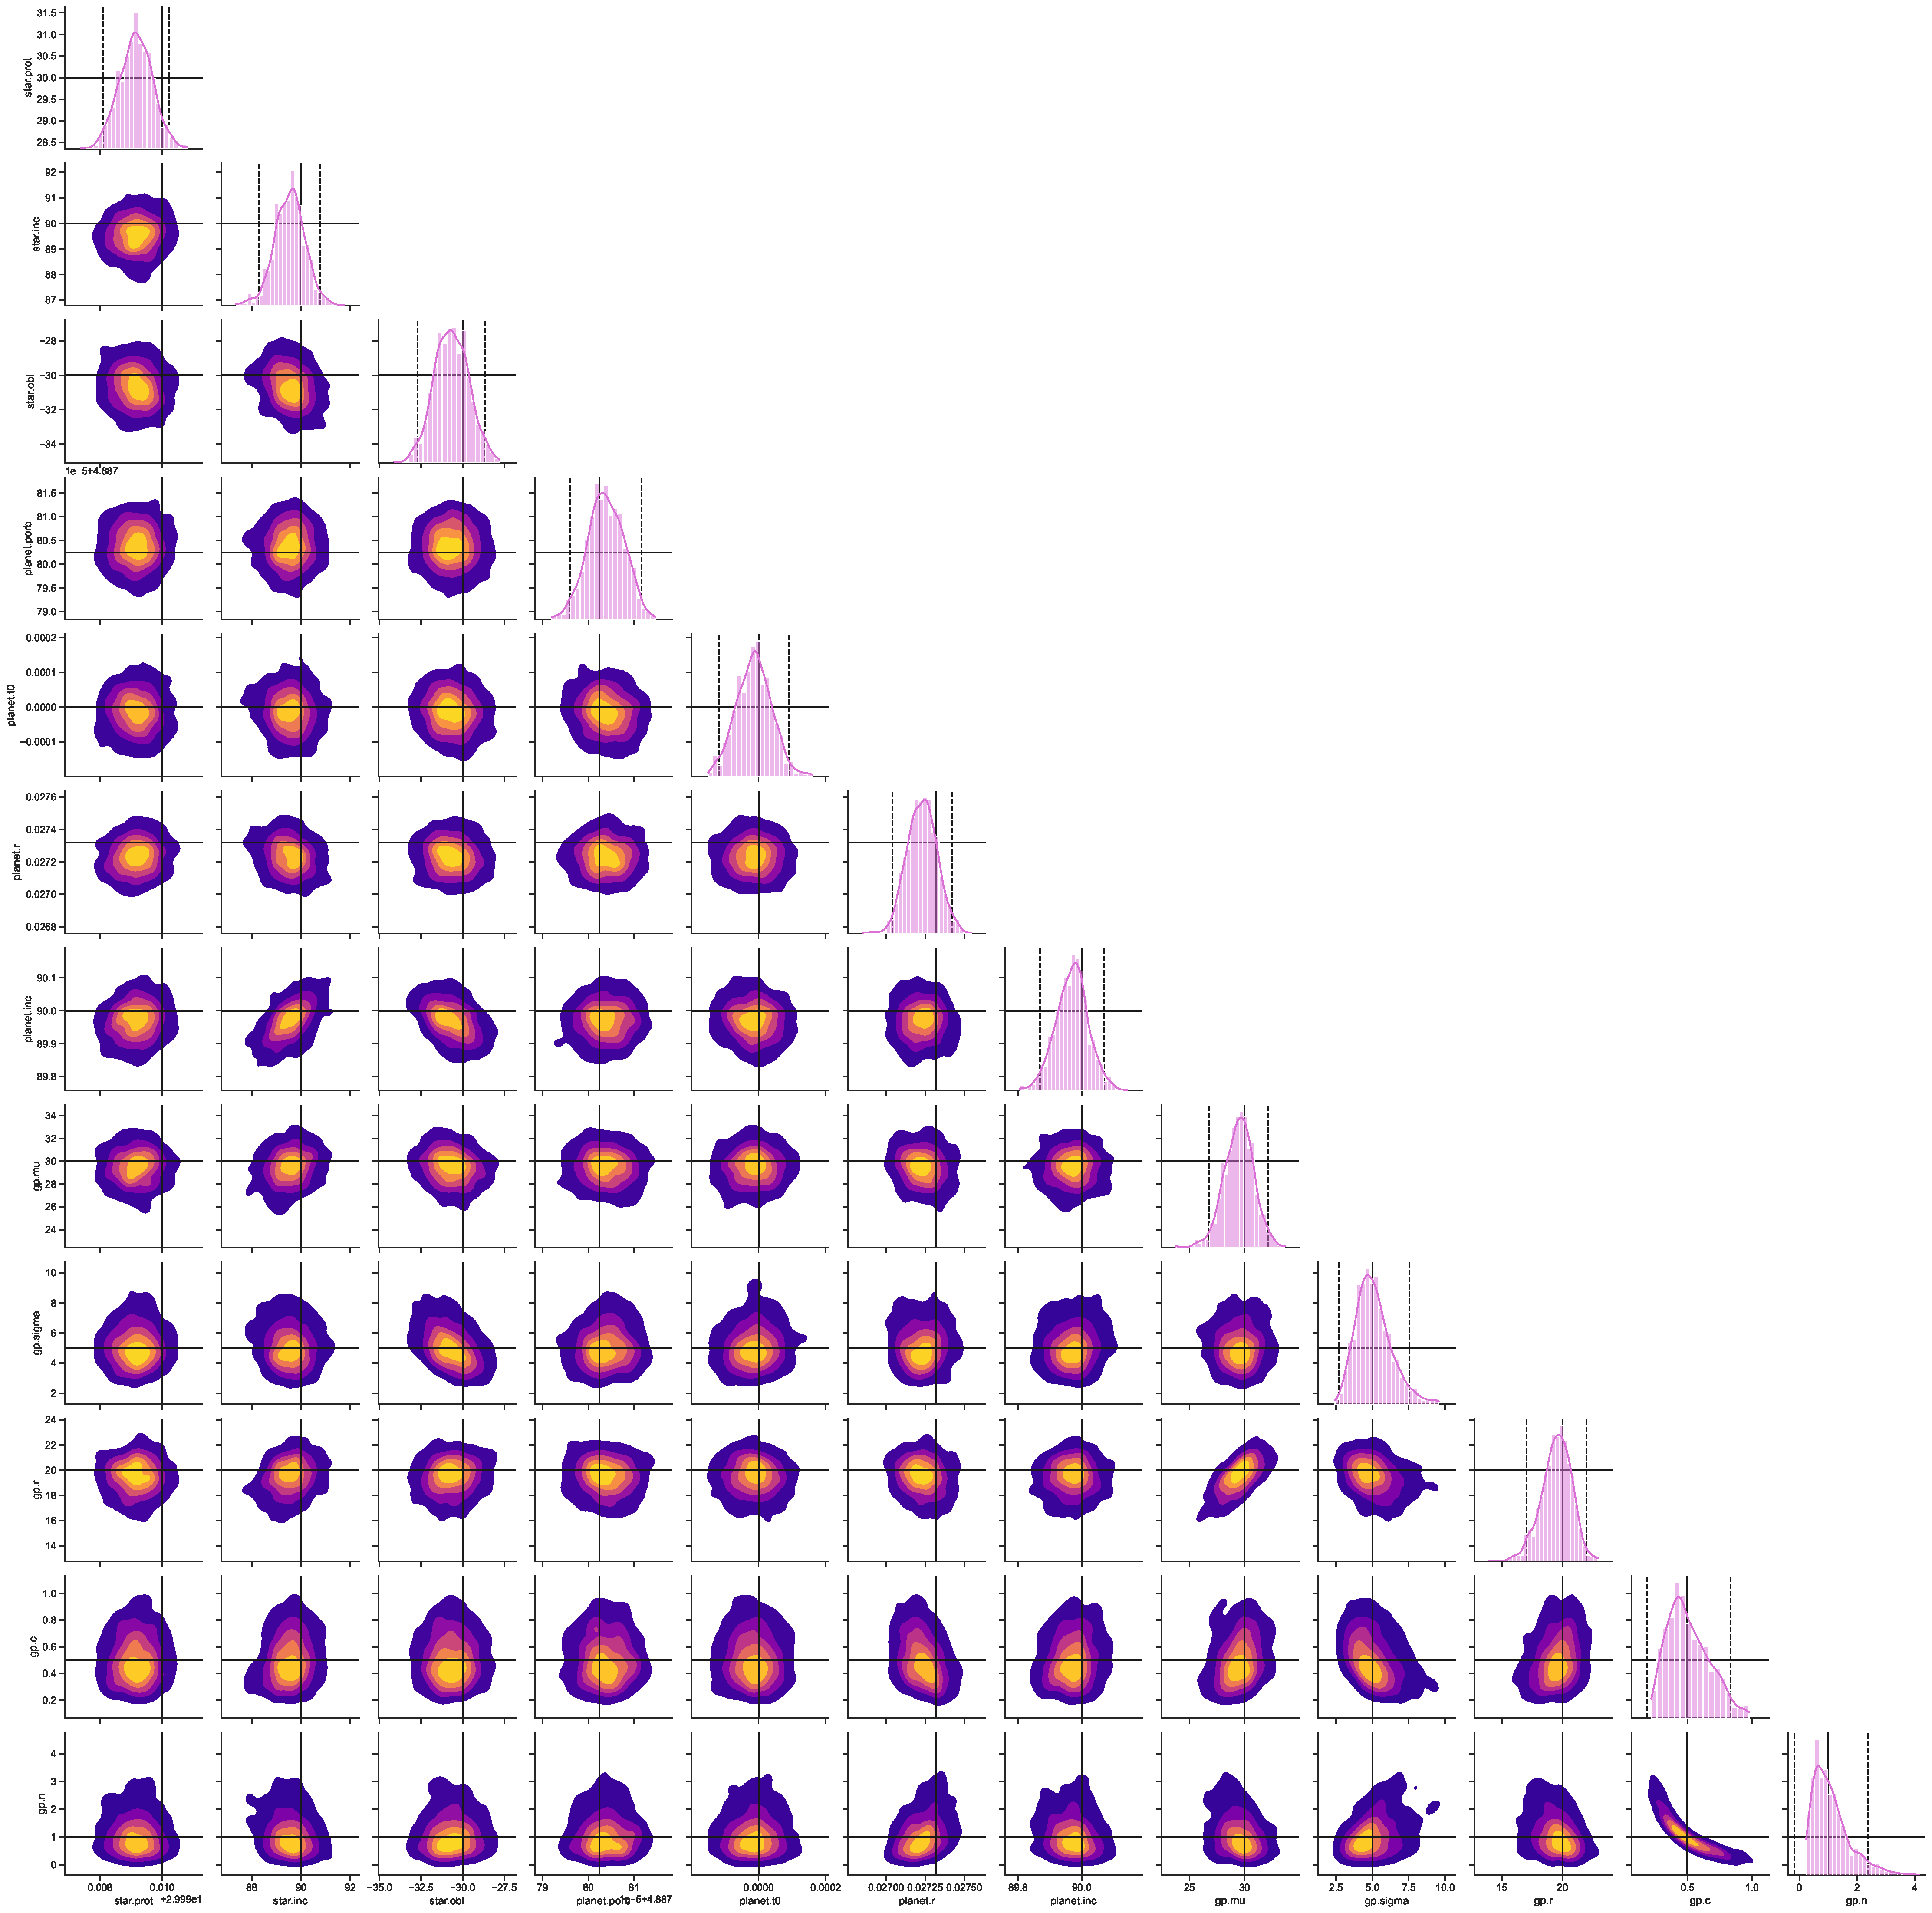
\includegraphics[width=\linewidth]{figures/SyntheticDataCorner.pdf}
%         \caption{
%             A synthetic dataset corner plot.
%         }
%         \label{fig:SyntheticDataCorner}
%     \end{centering}
% \end{figure}

\section{Results: synthetic datasets}
\label{sec:results-synthetic}
\subsection{Priors}
Before presenting the results, it is essential to elucidate the prior distributions employed throughout this work. 
We have implemented multiple priors in this work, carefully selected to maintain a balance between informativeness and generalizability. 
These priors serve to encapsulate our existing knowledge and assumptions about the parameters of interest, while allowing for sufficient flexibility 
to avoid computational cost.
\begin{itemize}
    \item $\sim\mathcal{U}(\rm low, \rm high)$: a uniform distribution.
    \item $\sim \rm Log \mathcal{U}(\rm low, \rm high)$: a log-uniform distribution.
    \item \textit{Planetary Inclination}: Considering that $i_p=\arccos{b}$, where $b$ is the impact parameter,
    the prior on the inclination is defined via the uniform prior $\sim\mathcal{U}(-b_{max}, -b_{max})$ on $b$, where $b_{max} = R_{\star} / a$.
    \item \textit{Period}: a prior on $P$ and $P_{\star}$. Instead of directly constraining the period, this prior works in log-space to ensure the period 
    remains positive and to make the distribution more symmetric. The actual prior is a uniform distribution in log-space, bounded by the log of the true 
    value plus or minus some fraction. The final period is determined by exponentiating the result of this log-uniform distribution, 
    which effectively creates a kind of log-uniform prior on the period itself.
    \item \textit{Stellar Angle}: a normal distribution on orientation vectors $\tilde{x}$ and $\tilde{y}$ and a half-normal distribution on $\tilde{z}$. See Section
    \ref{sec:obl-inc} for the full explanation.
\end{itemize}

\subsection{Experiment I: non-evolving surface}
\label{sec:experiment1}
To verify the proper calibration of our model, we evaluate its performance using synthetic data, which is created through the following process.
We create a system consisting of a star and a planet, each of them have some orbital parameters presented in Table \ref{tab:LongPriors}. 
The \textit{true} map is just a random draw from a from the process evaluated up to spherical harmonic degree
$l_{max} = 15$ and conditioned on different values of the hyperparameter vector $\pmb{\theta}_\bullet$ (Table \ref{tab:LongPriors}). Figure \ref{fig:experiment-1-map} 
illustrates the setup of Experiment I. The upper panel displays the "true" map used in the experiment, which represents the underlying reality that 
the model aims to reconstruct. This map represents the brightness distribution across the star's surface. We generated 90 days of observations with a 2-minute
cadence, and then we binned the out-of-transit flux to speed up the sampling process.
\begin{figure*}[ht!]
    % \script{experiment-1-true-map.py}
    \begin{centering}
        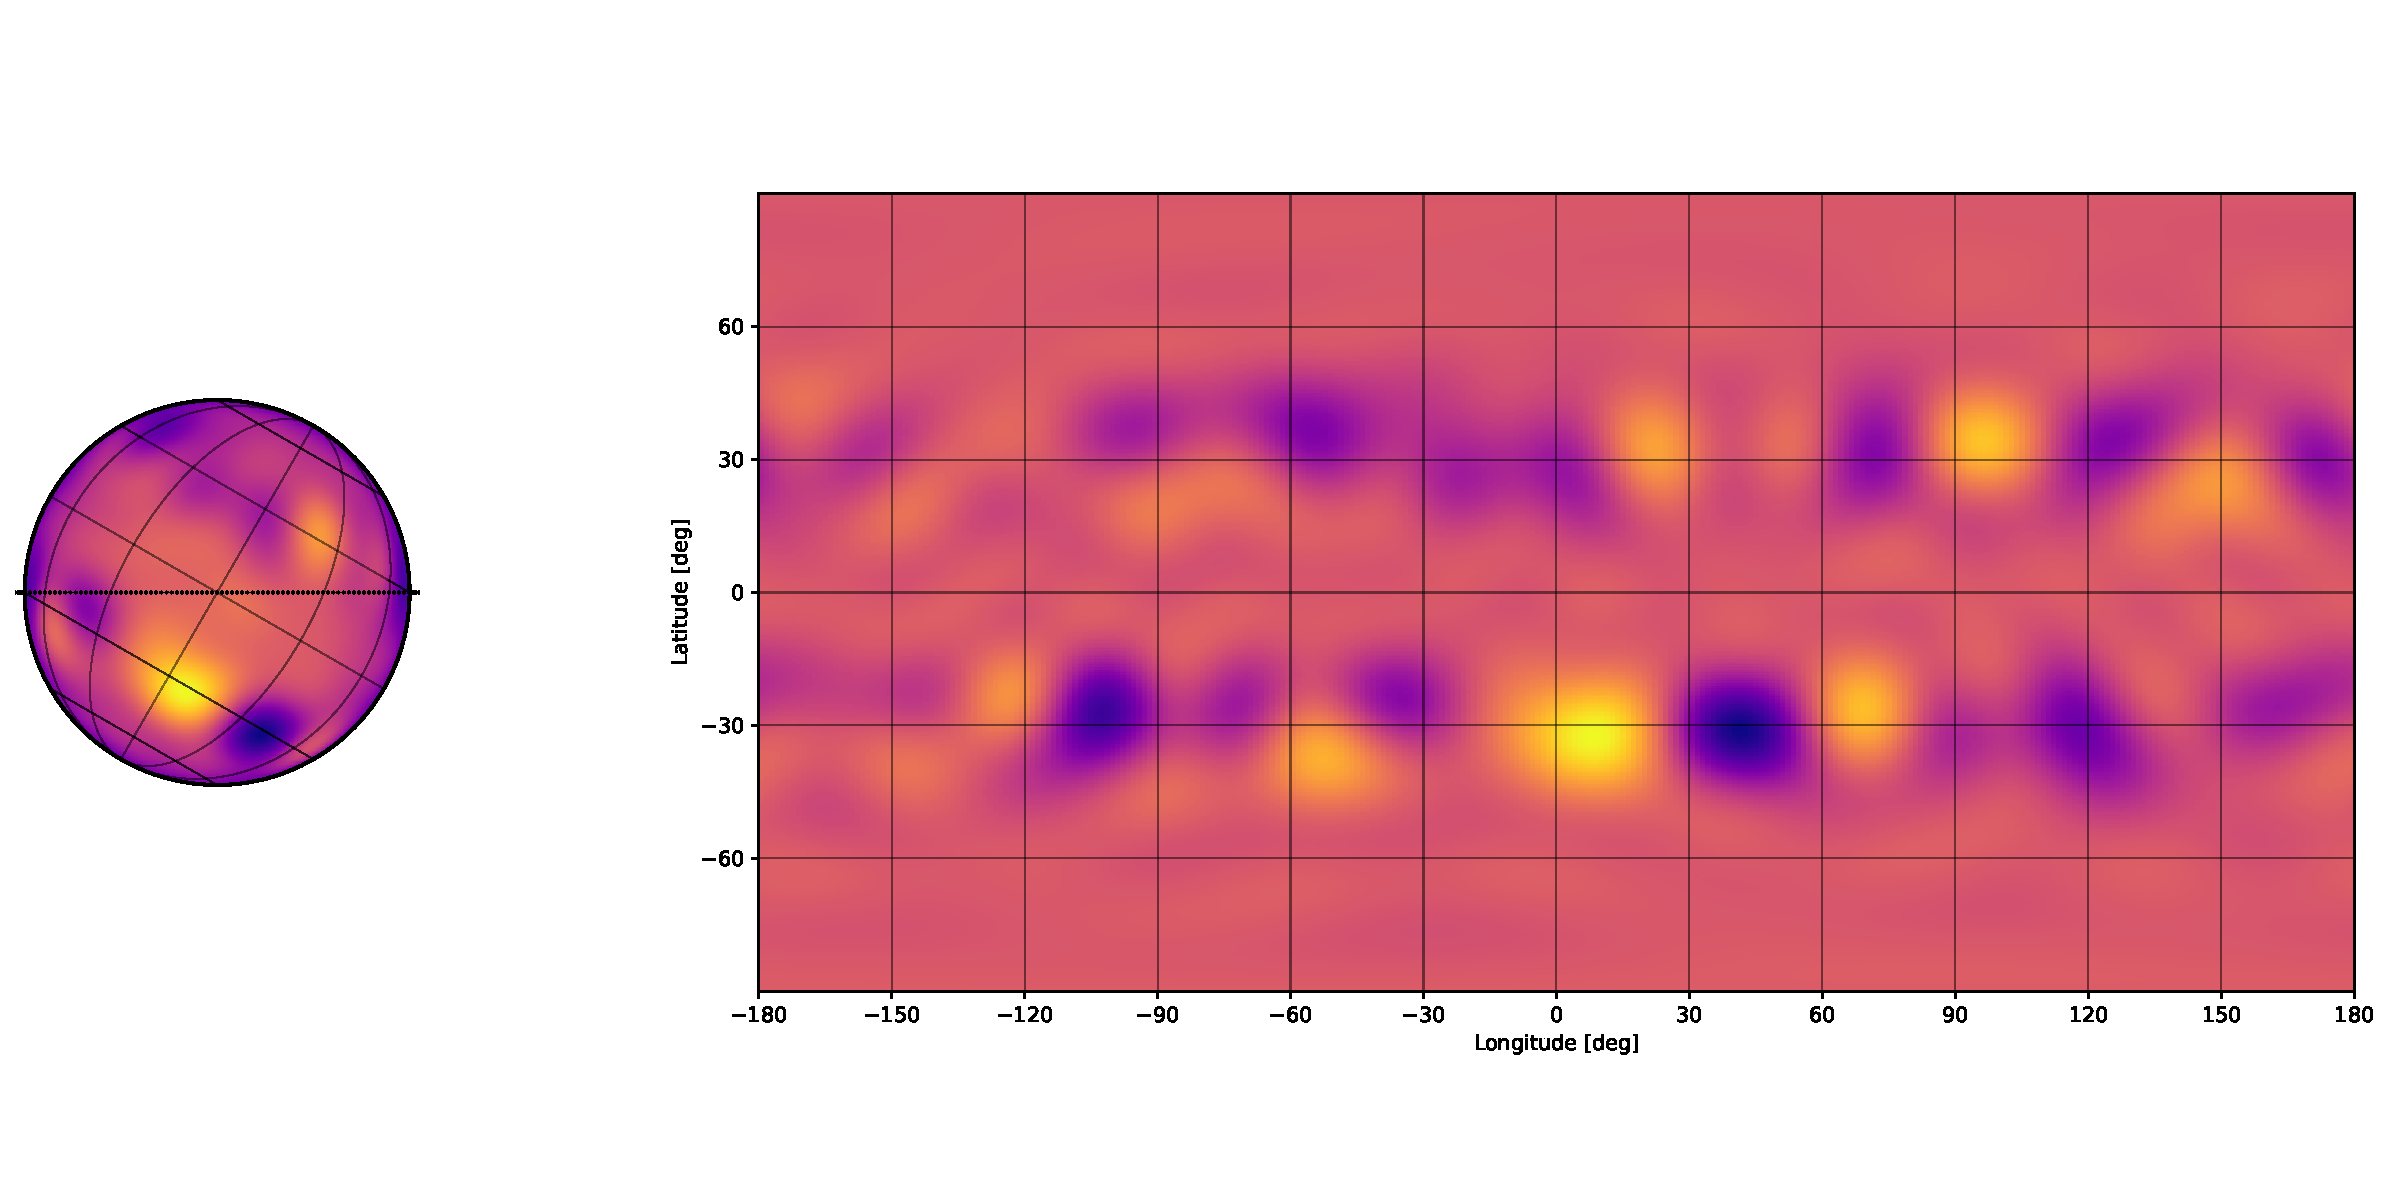
\includegraphics[width=\linewidth]{figures/experiment-1-true-map.pdf}
        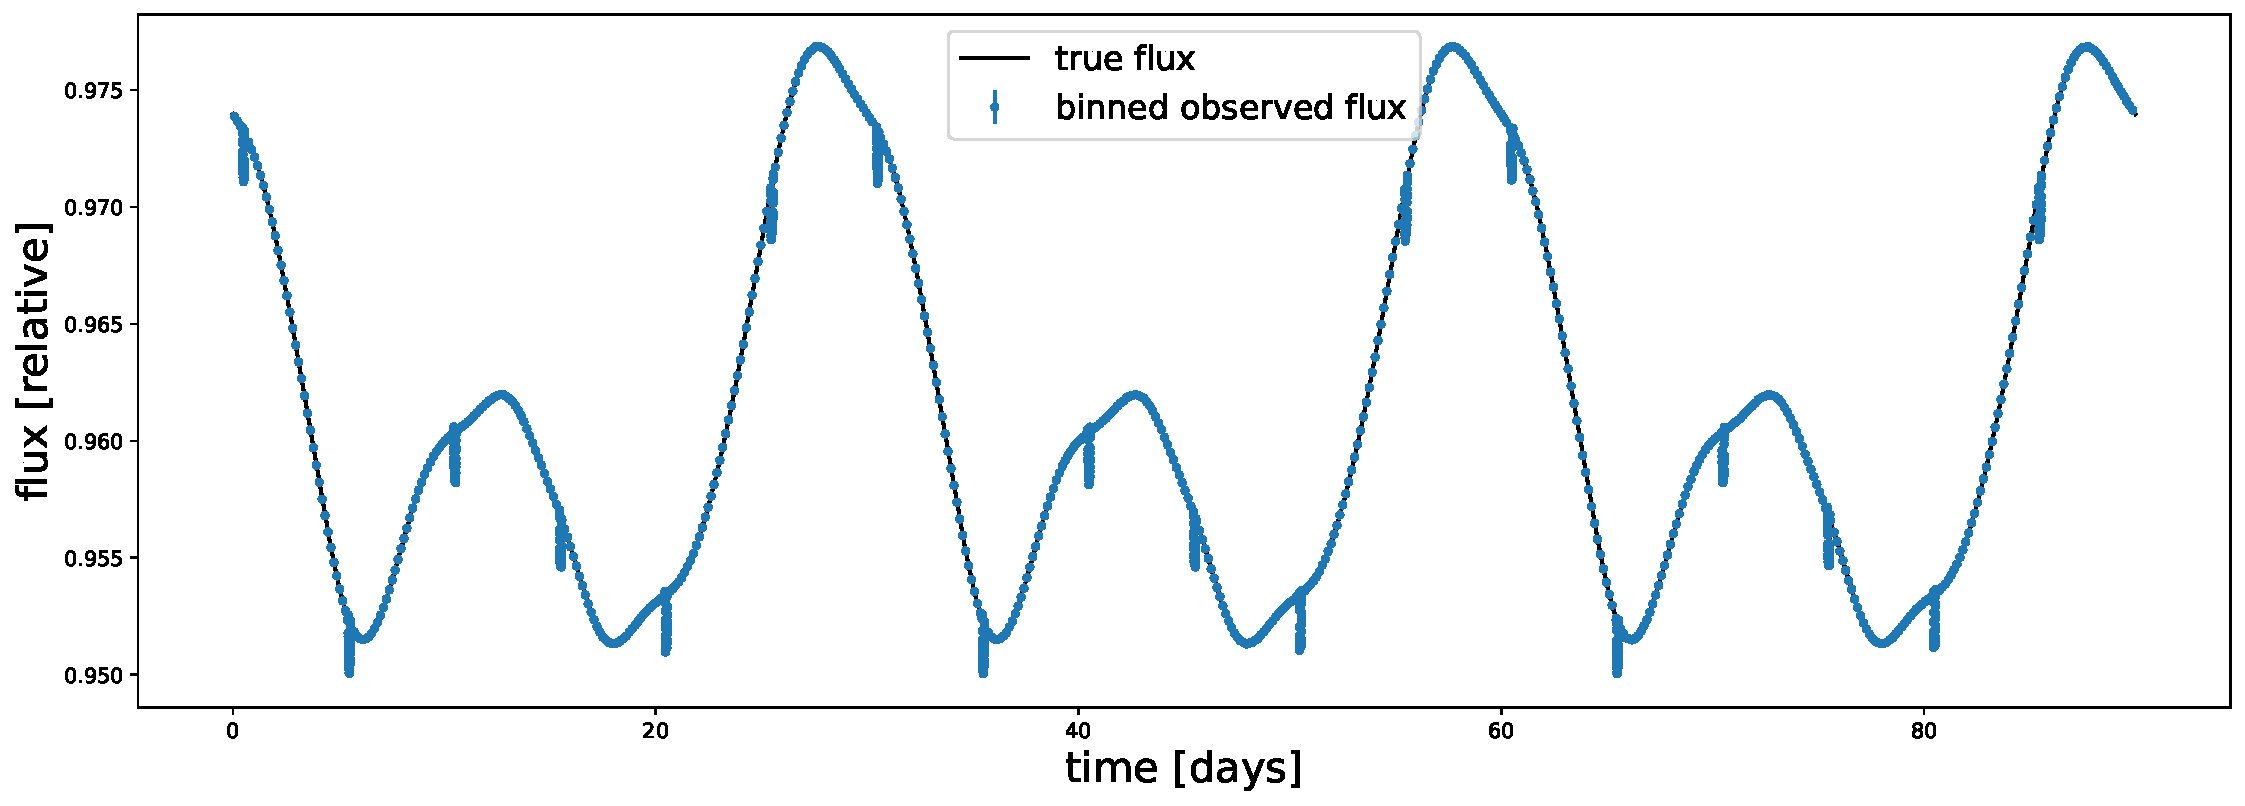
\includegraphics[width=\linewidth]{figures/experiment-1-lc.pdf}
        \caption{
            The upper panel shows the \textit{true} map for the Experiment I of this paper. The black dots on the map indicate the trajectory of the 
            planet as it moves across the face of the star during the transit event. The left panel 
            shows the stellar map along with its orientation on the sky and the right panel shows the rectangular projection of the map. 
            The bottom panel is the generated light curve. The black line is the \textit{true} light curve and the blue dots show the binned light curve
            that's used in the model.
        }
        \label{fig:experiment-1-map}
    \end{centering}
\end{figure*}

We used No-U-Turn Sampling, a variant of Hamiltonian Monte Carlo \citep[NUTS;][]{Duane1987,Hoffman2011} to do posterior inference on our synthetic dataset.

We use several parameters in our sampling process: $i_p$ (the planetary inclination), $e$ (its eccentricity), $P$ (its orbital period),
$t_0$ (start of the transit time), $R_p/R_\star$ (ratio of planetary to stellar radius), $u_1$ and $u_2$ (limb darkening coefficients),
$i_\star$ (stellar inclination), $\lambda_\star$ (stellar obliquity), $P_\star$ (stellar rotational period), $\mathbb{n}$ (the number of spots), 
$\mathbb{c}$ (their contrast), $\mathbb{r}$ (their radius), and $\mathbb{a}$ and $\mathbb{b}$ (parameters of the Beta distribution that describe 
how the spots are spread across latitudes).  

We use Equation \ref{eq:log-likeRodrigo} as our log likelihood term. The results are shown on Figure \ref{fig:experiment-1-map-corner-all},
where we correctly infer almost all five parameters within $\sim 2$ standard deviations. The only parameters that are not constrained too well are 
planetary eccentricity $e$ and the radius of spots $\mathbb{r}$, but they are still fairly close to the true values: the true value for the
eccenticity is 0.2 while the inferred median value is 0.225, and the true value for the radius of spots is $10^\circ$ while the inferred median value is
$14.3^\circ$. 

To visually demonstrate the performance of our model, Figure \ref{fig:experiment-1-map-comparison} presents a comprehensive comparison between 
the true stellar surface used in our synthetic data generation and the inferred surface map from our analysis, alongside the resulting light curve fit and 
transit details. Of particular interest are the three consecutive transits shown in detail on the right panel. These zoomed-in views highlight our 
model's ability to precisely fit transit events, including subtle spot-crossing phenomena. The spot-crossing events, visible as brief increases in brightness 
during the transits, are well-captured by our model. It can be seen that true and inferred maps are not \emph{exactly} the same, but share the same surface features -- i.e. bright spots at the
same locations, same active latitudes, etc. -- which still explains the surface of the star.
%
\begin{figure*}[hbt!]
    % \script{experiment-1-true-map.py}
    \begin{centering}
        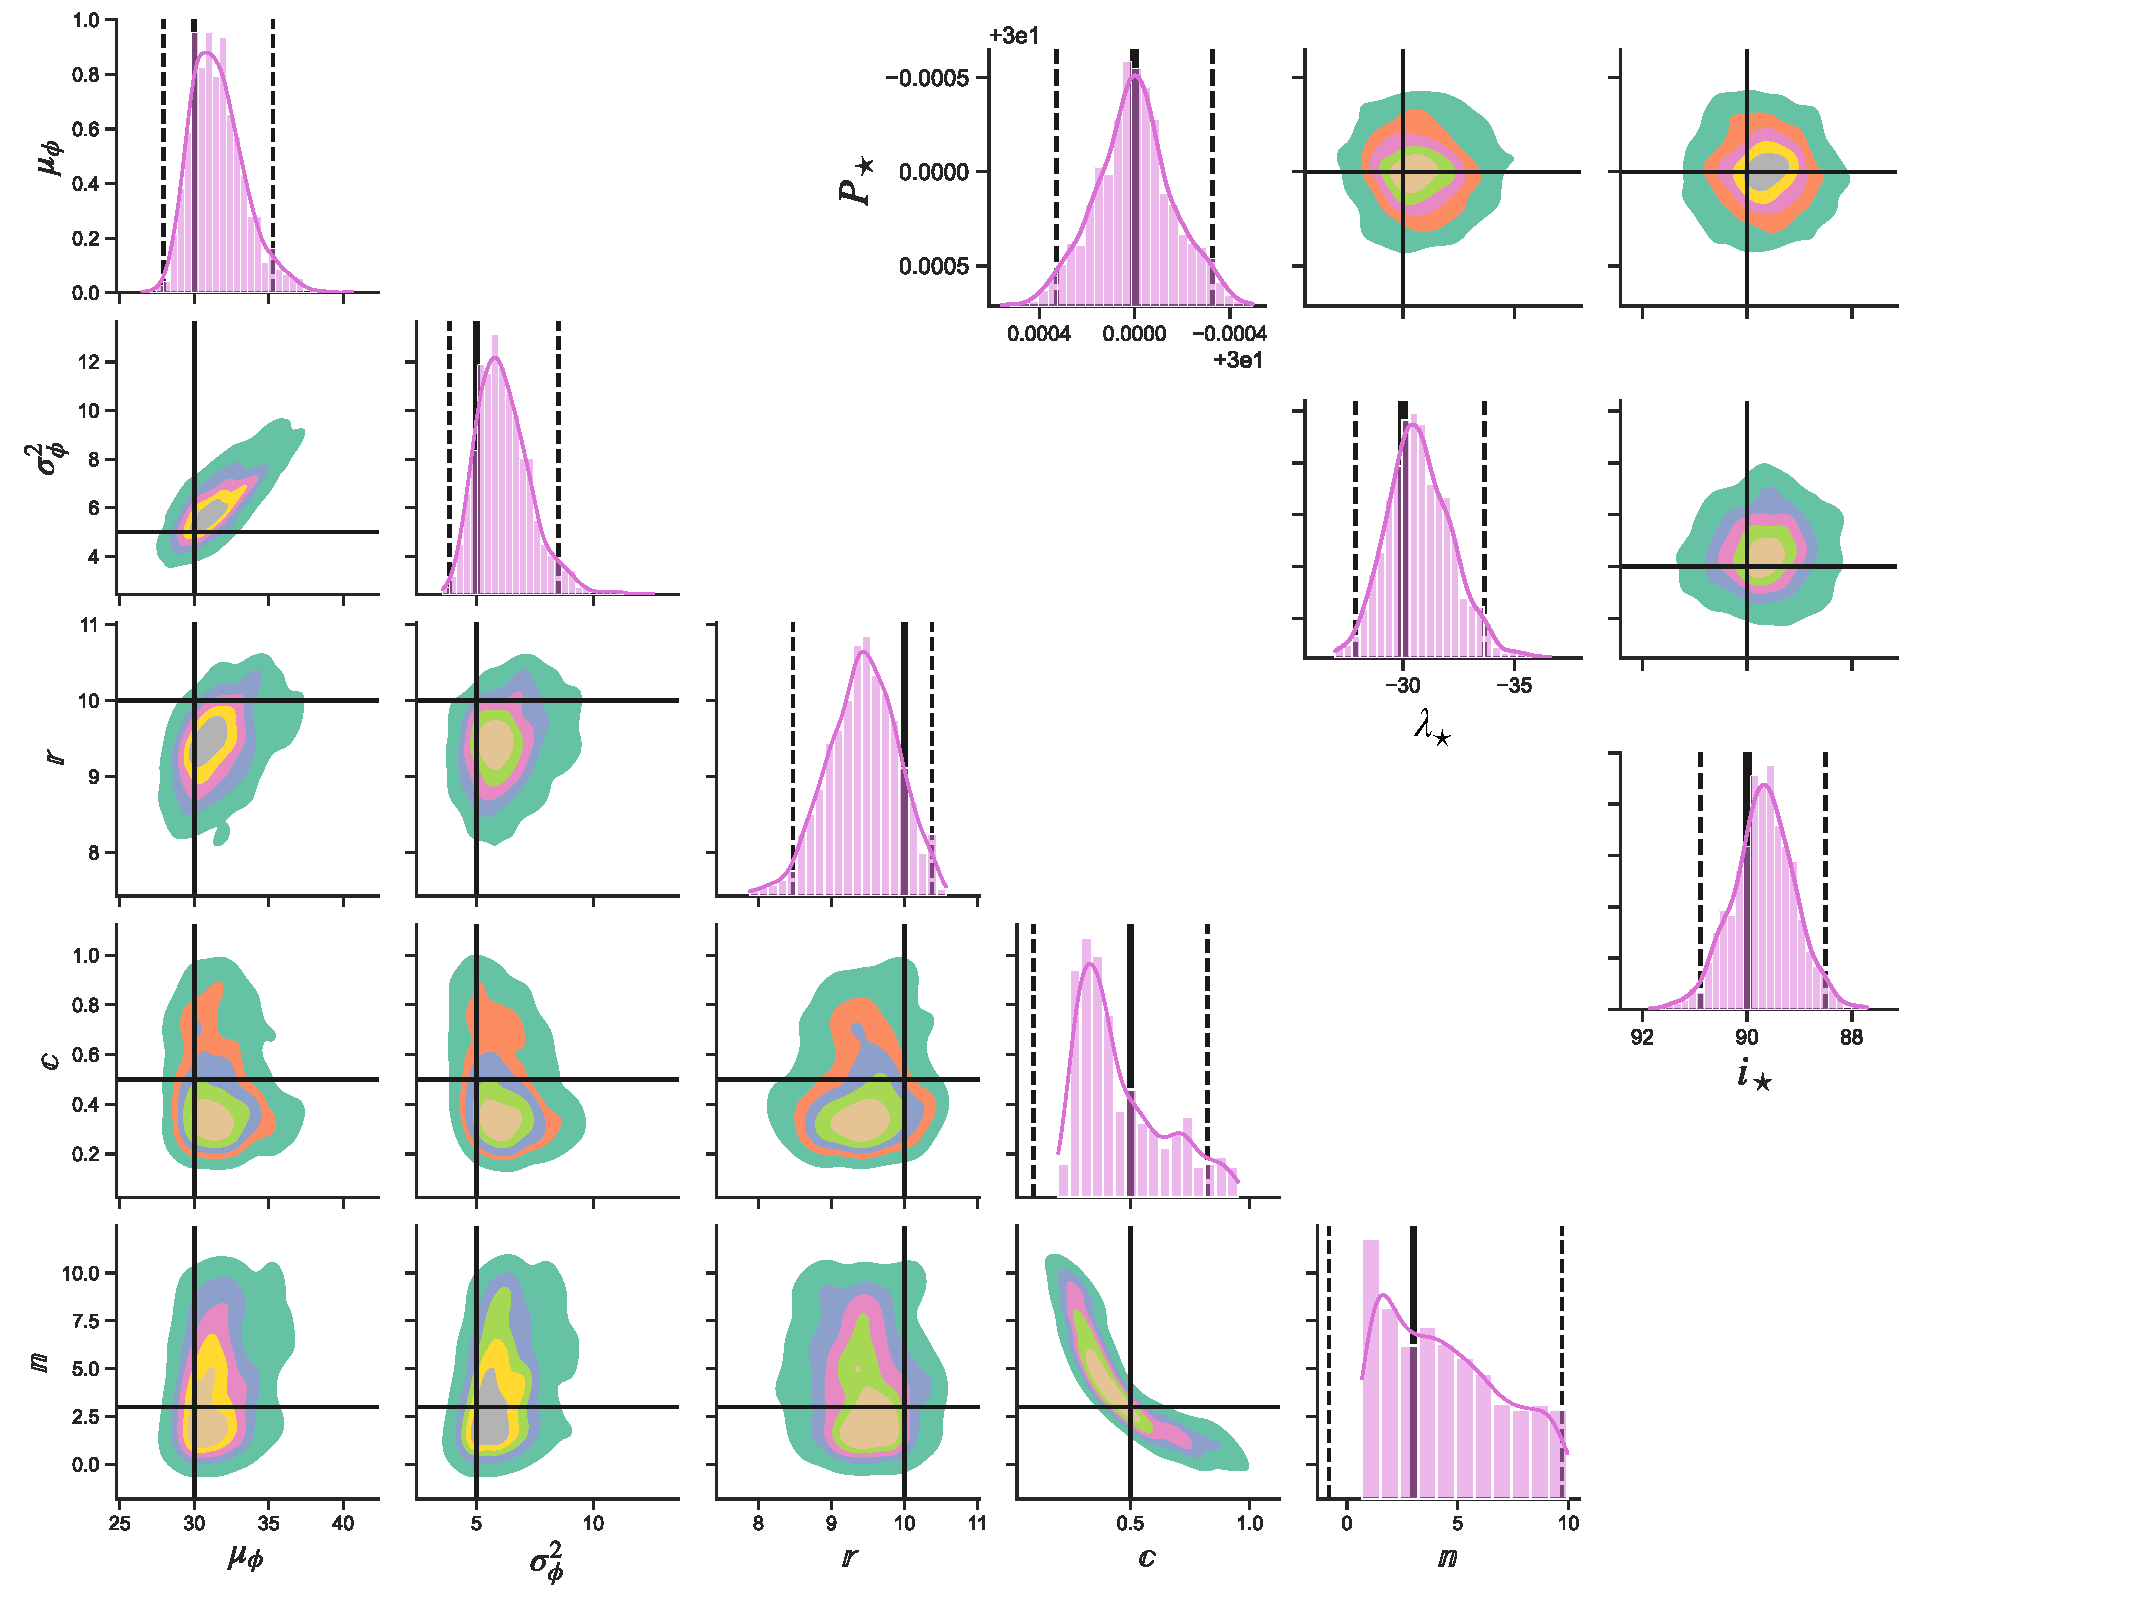
\includegraphics[width=\linewidth]{figures/experiment-1-corner-gp-star.pdf}
        \caption{
            Posterior distributions for the all the parameters $\pmb{\Theta}$ for the synthetic data run 
            (Table \ref{tab:LongPriors} and Figure \ref{fig:experiment-1-map}). The axes span the entire prior volume, and 
            the black lines indicate the true (input) values, the dashed black lines indicate 2 standard deviations.
        }
        \label{fig:experiment-1-map-corner-all}
    \end{centering}
\end{figure*}
%
\begin{figure*}[hbt!]
    % \script{experiment-1-true-map.py}
    \begin{centering}
        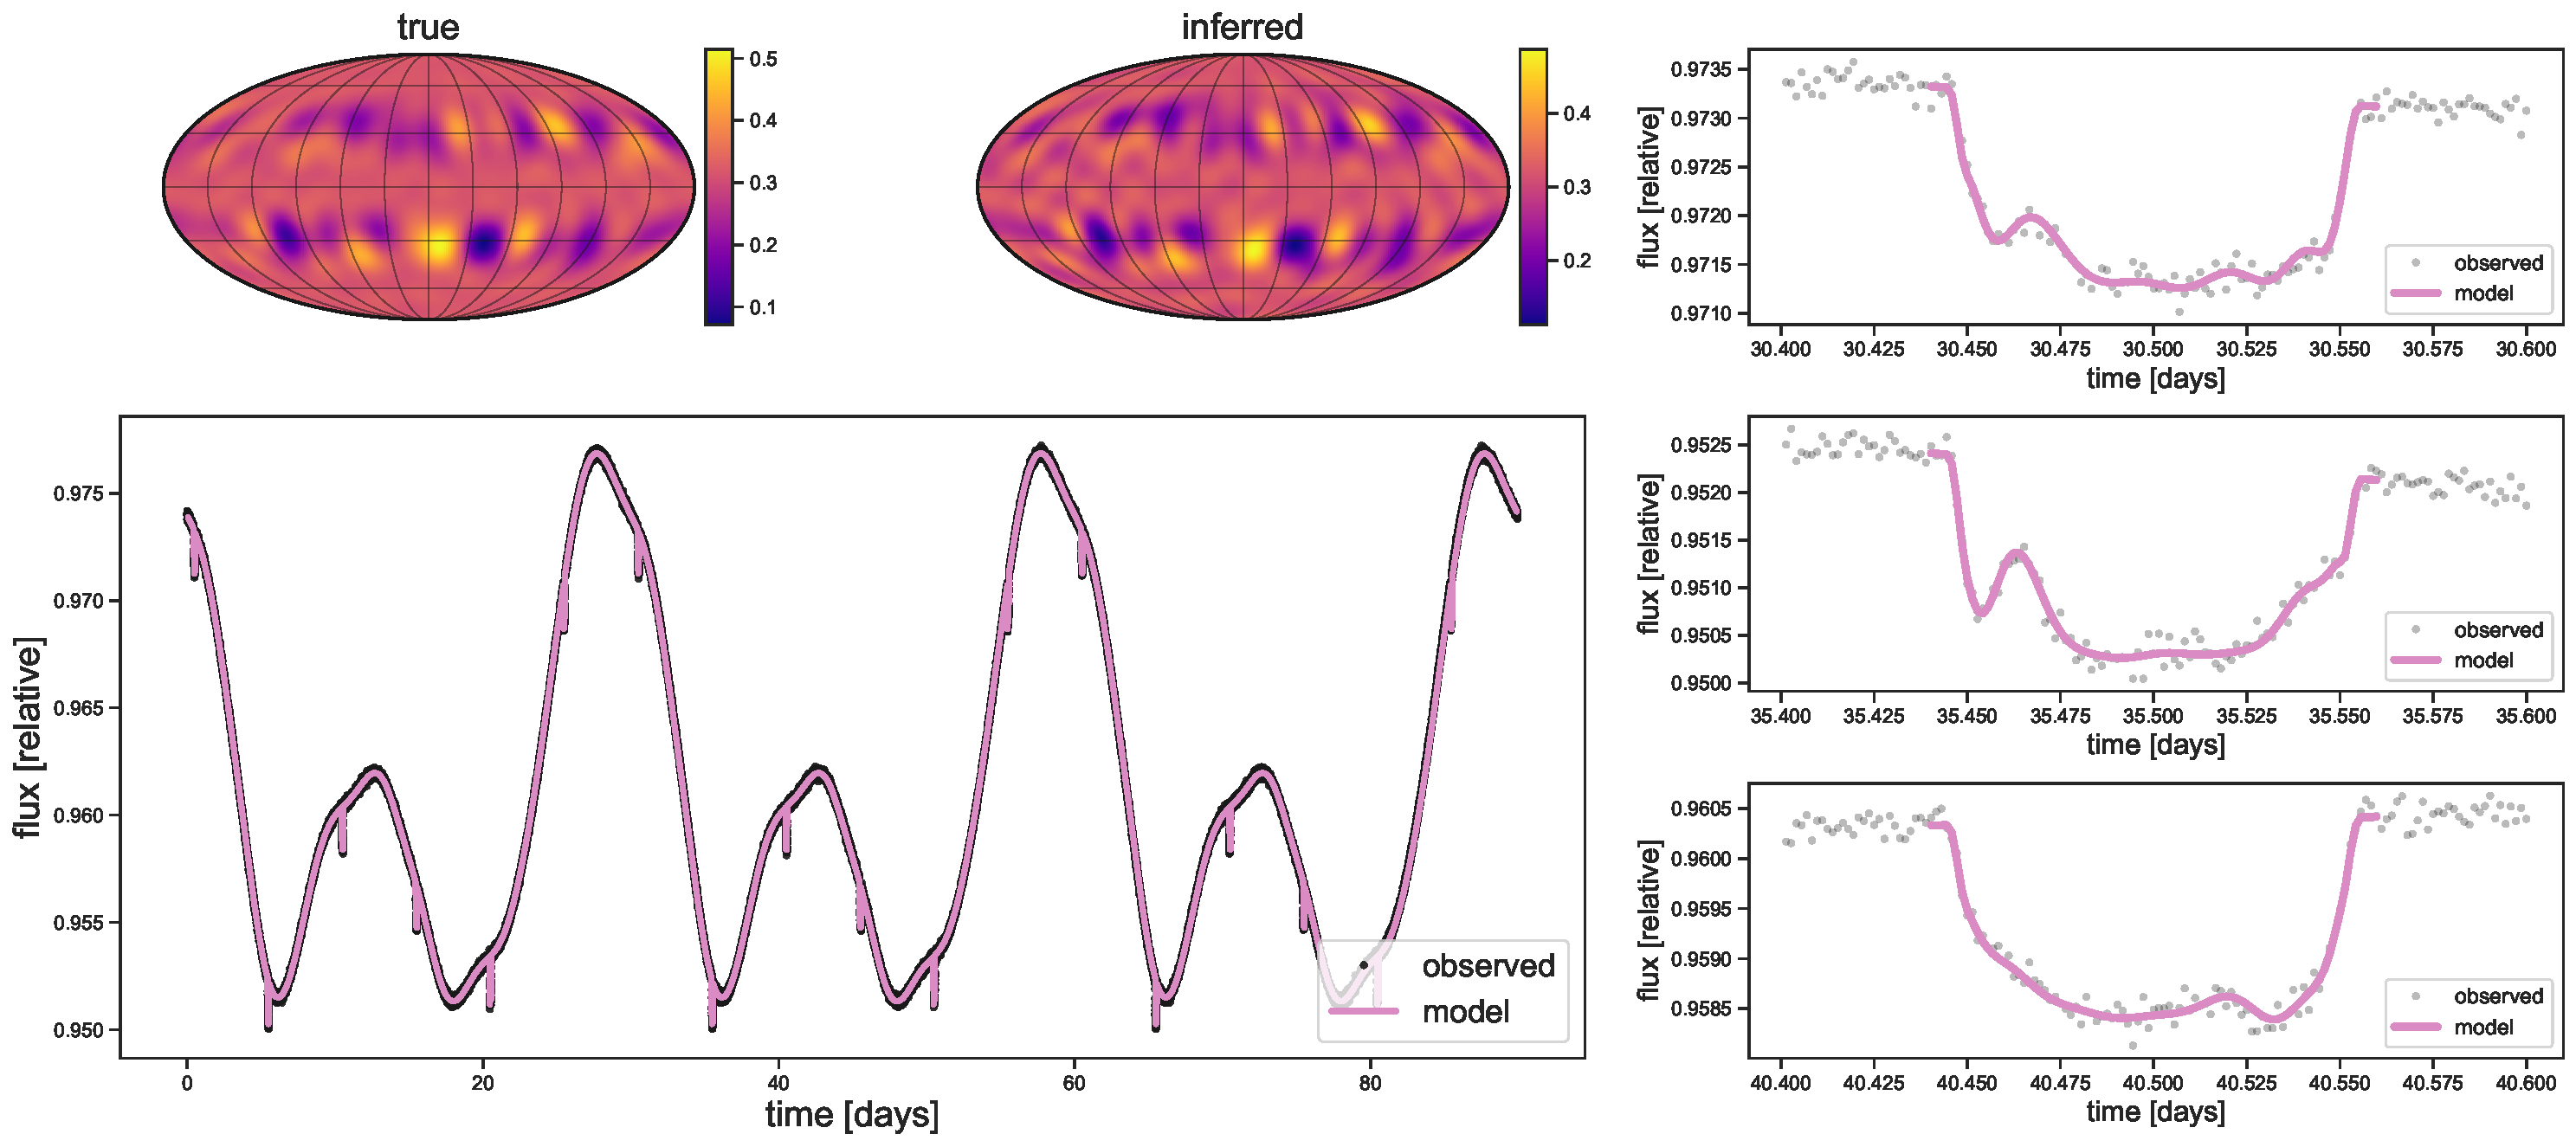
\includegraphics[width=\linewidth]{figures/experiment-1-map-comparison.pdf}
        \caption{
            Comparison of true and inferred stellar surface maps, light curve fit, and transit details. Top panel: the true stellar surface map used to 
            generate synthetic data and the inferred stellar surface map, representing the mean of 1000 posterior samples. Color scales represent spot 
            intensity. The similarity between true and inferred maps demonstrates the model's capability to recover the overall spot distribution. Bottom panel:
            Full light curve comparison. Black points show the synthetic data with added noise. The pink line represents the best-fit model, 
            computed as the mean of 1000 posterior samples. Right panel (three rows): zoom-in views of three consecutive transits. Black points are data, 
            pink lines show the best-fit model. Note the spot-crossing events visible as brief brightness increases during transits. 
            The light curve fit shows strong agreement with the data over the full time series, while the transit close-ups highlight the model's ability 
            to capture subtle spot-crossing events and their evolution over consecutive transits.
        }
        \label{fig:experiment-1-map-comparison}
    \end{centering}
\end{figure*}
%
To evaluate the effectiveness of our model in recovering the underlying spot distribution, we examined the posterior distributions of spot latitudes 
derived from our synthetic data analysis. Figure \ref{fig:experiment-1-acttive-lats} illustrates these results, and the constraints we can place on 
stellar spot distributions. In Figure \ref{fig:experiment-1-acttive-lats}, each pink curve represents a Beta distribution PDF for spot latitude. 
These curves are generated using parameters sampled from the posterior distributions of $\mu_\phi$ and $\sigma_\phi$, which characterize the 
latitude distribution in our model. The collection of pink curves effectively creates a distribution that quantifies our inferred knowledge about 
how spots are distributed across the stellar surface in our dataset. The variability among these pink curves reflects the uncertainty in our inference. 
Regions where the curves are more tightly clustered indicate greater certainty in our estimates, while areas with more spread suggest higher uncertainty. 
This visualization allows us to assess not just a single "best-fit" distribution, but the full range of plausible distributions consistent with our data and model.
The black curve in Figure \ref{fig:experiment-1-acttive-lats} represents the true underlying distribution used to generate the synthetic spot data, 
with parameters as specified in Table \ref{tab:LongPriors}. The general agreement between the ensemble of pink curves and this 
true distribution is encouraging, demonstrating that our model can successfully recover the input spot latitude distribution within the 
uncertainties of the inference process.
%
\begin{figure*}[hbt!]
    % \script{experiment-1-true-map.py}
    \begin{centering}
        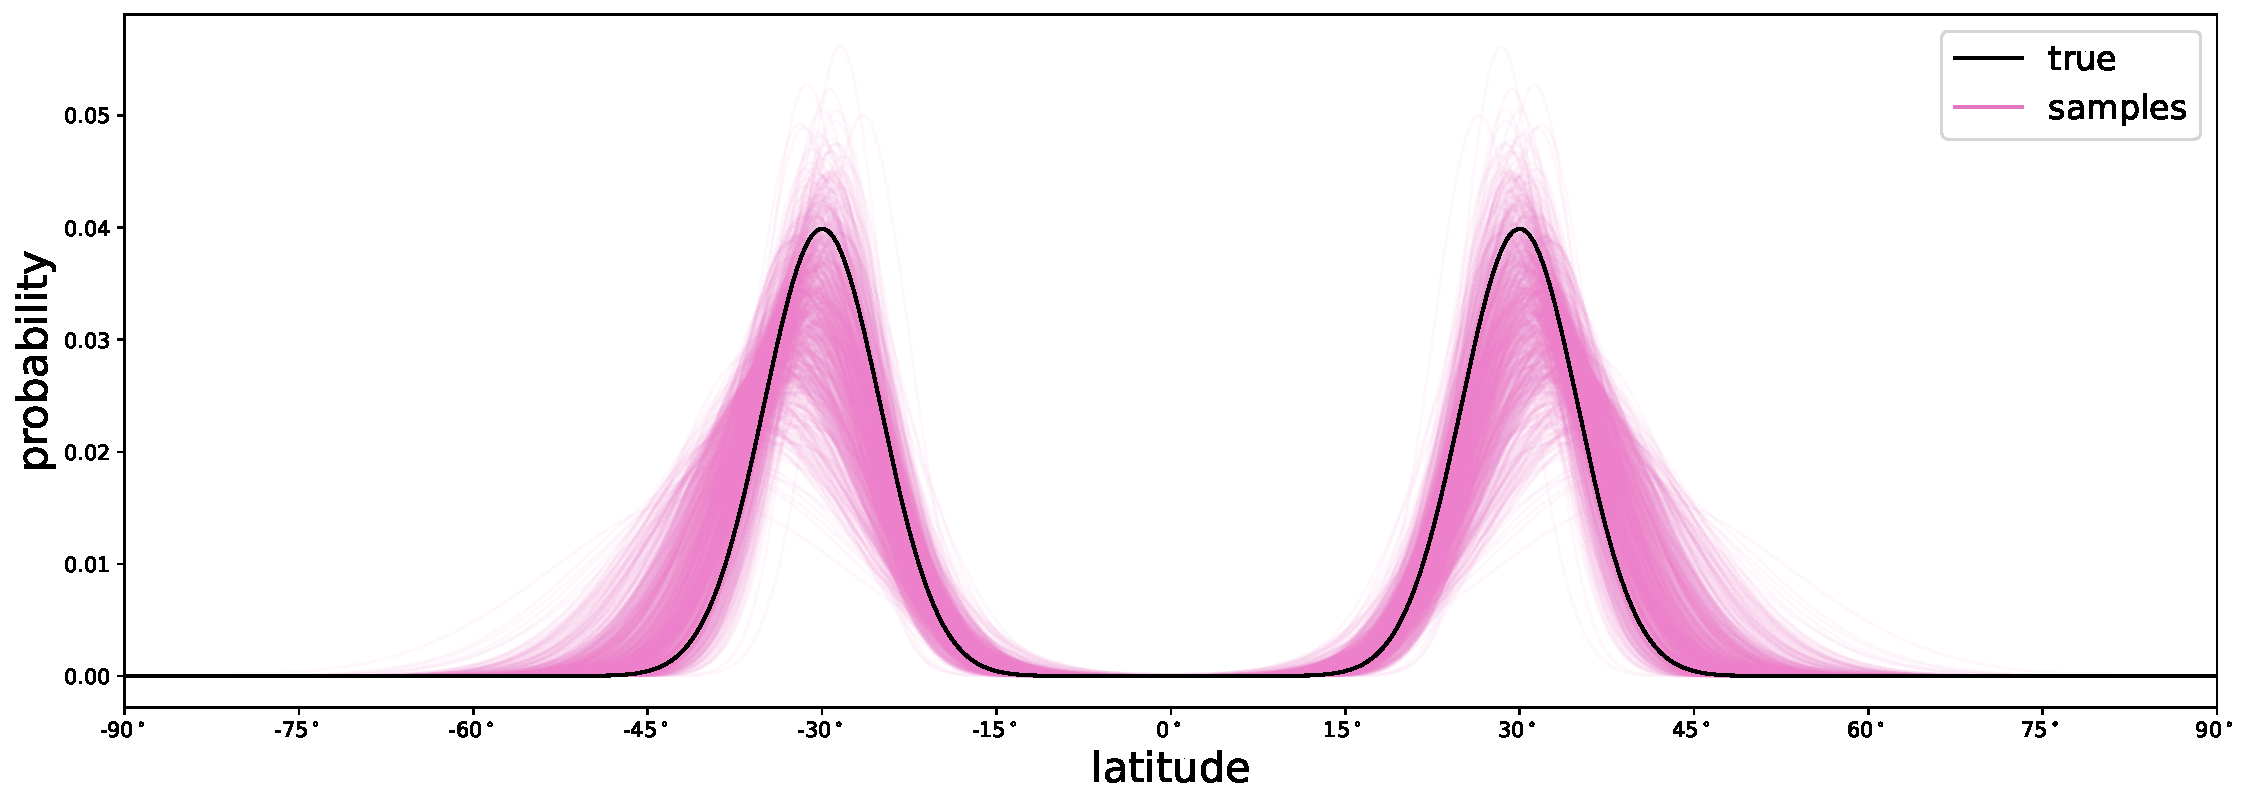
\includegraphics[width=\linewidth]{figures/experiment-1-active-lats.pdf}
        \caption{
            Posterior distributions of spot latitudes derived from synthetic data analysis. The pink curves represent individual Beta distribution 
            probability density functions (PDFs) for spot latitude, each generated using parameters sampled from the posterior distributions of 
            $\mu_\phi$ and $\sigma_\phi$ (Figure \ref{fig:experiment-1-map-corner-all}). The ensemble of pink curves illustrates the range of 
            plausible spot latitude distributions, effectively quantifying our inferred knowledge about spot distribution patterns across the stellar surface 
            in our dataset. The black curve shows the true underlying distribution used to generate the synthetic spot data (parameters given in Table 
            \ref{tab:LongPriors}). Note the general agreement between the inferred distributions and the true distribution, 
            demonstrating the model's ability to recover the input spot latitude distribution within the uncertainties of the inference process.
        }
        \label{fig:experiment-1-acttive-lats}
    \end{centering}
\end{figure*}
%
%
\begin{table}[]
    \vspace{0.5cm}
    \centering
    \caption{The free parameters for the synthetic data in Section \ref{sec:experiment1}, their true values, and their priors.}
    \begin{tabular}{llll}
    \hline
    Parameter                                 & True value            & Prior distribution                   & Inferred value    \\ \hline\hline
    $i_p$                                     & $90^\circ$            & Planetary Inclination                & $90.04^{+0.104}_{-0.089}$                   \\
    $e$                                       & $0.2$                 & $\sim\mathcal{U}(0, 0.5)$            & $0.224 \pm 0.001$                     \\
    $P$                                       & $5$ days              & Period                               & $5.0^{+7\times10^{-6}}_{-6.45\times10^{-6}}$                       \\
    $t_0$                                     & $0.5$                 & $\sim\mathcal{U}(-0.6, 0.6)$         & $0.5^{+10^{-4}}_{-9.8\times10^{-5}}$                       \\
    $R_p / R_\star$                           & $0.04$                & $\sim \rm Log \mathcal{U}(0.02, 0.08)$ & $0.04 \pm 2\times10^{-4}$                         \\ 
    $u_1$                                     & $0.4$                 & $\sim\mathcal{U}(0, 0.6)$            & $0.38^{+0.07}_{-0.06}$                         \\ 
    $u_2$                                     & $0.26$                & $\sim\mathcal{U}(0, 0.4)$            & $0.29 \pm 0.06$                         \\ \hline
    $i_\star$                                 & $90^\circ$            & Stellar Angle                        & $89.68^{+0.6}_{-0.56}$                      \\
    $\lambda_\star$                           & $-30^\circ$           & Stellar Angle                        & $-30.67^{+1.33}_{-1.48}$                           \\
    $P_\star$                                 & $30$ days             & Period                               & $30\pm 2 \times10^{-4}$                       \\ \hline
    $\mathbb{r}$                              & $10^\circ$            & $\sim\mathcal{U}(5, 25)$             & $9.44^{+0.447}_{-0.497}$                           \\
    $\mathbb{c}$                              & $0.5$                 & $\sim\mathcal{U}(0.01, 1)$           & $0.46^{+0.28}_{-0.1}$                               \\
    $\mathbb{n}$                              & $3$                   & $\sim\mathcal{U}(0, 10)$             & $4.45^{+3.53}_{-2.6}$                               \\
    $\mu_\phi$                                & $30^\circ$            & $\sim\mathcal{U}(0, 1)$ on $\mathbb{a}$ and $\mathbb{b}$ & $31.6^{+1.99}_{-1.52}$                               \\
    $\sigma^2_\phi$                           & $5^\circ$             & $\sim\mathcal{U}(0, 1)$ on $\mathbb{a}$ and $\mathbb{b}$ & $6^{+1.2}_{-0.95}$                      \\ \hline
    \label{tab:LongPriors}
    \end{tabular}
\end{table}
%

Finally, it is important to note that all results presented in this analysis have been carefully adjusted to account for the inclination and obliquity 
degeneracy discussed in Section \ref{sec:obl-inc}. As discussed earlier, a system with stellar inclination $i_\star$ and obliquity $-\lambda_\star$ 
produces identical light curves to a system with inclination $180^\circ-i_\star$ and obliquity $\lambda_\star$. In our analysis process, 
when we encounter a solution that gives the obliquity $\lambda_\star$ instead of $-\lambda_\star$, we systematically transform the results. 
Specifically, we change the inclination to $180^\circ-i_\star$ for visualization purposes in Figure \ref{fig:experiment-1-map-corner-all}. 
This approach ensures consistency in our reported results and allows for meaningful comparisons across different systems or models. 
By explicitly addressing this degeneracy, we provide a more robust and physically interpretable set of results, avoiding potential ambiguities in the 
orientation of the stellar spin axis relative to the planetary orbit. To show this explicitly, in Figure \ref{fig:experiment-1-inf-map-comparison}
we plot the inferred maps, where the left one is the map with the degeneracy accounted for, and the right one is the map with the actual inferred values 
for obliquity and inclination (degeneracy is not accounted for). The two maps are inverses of eahc other.

%
\begin{figure*}[hbt!]
    % \script{experiment-1-true-map.py}
    \begin{centering}
        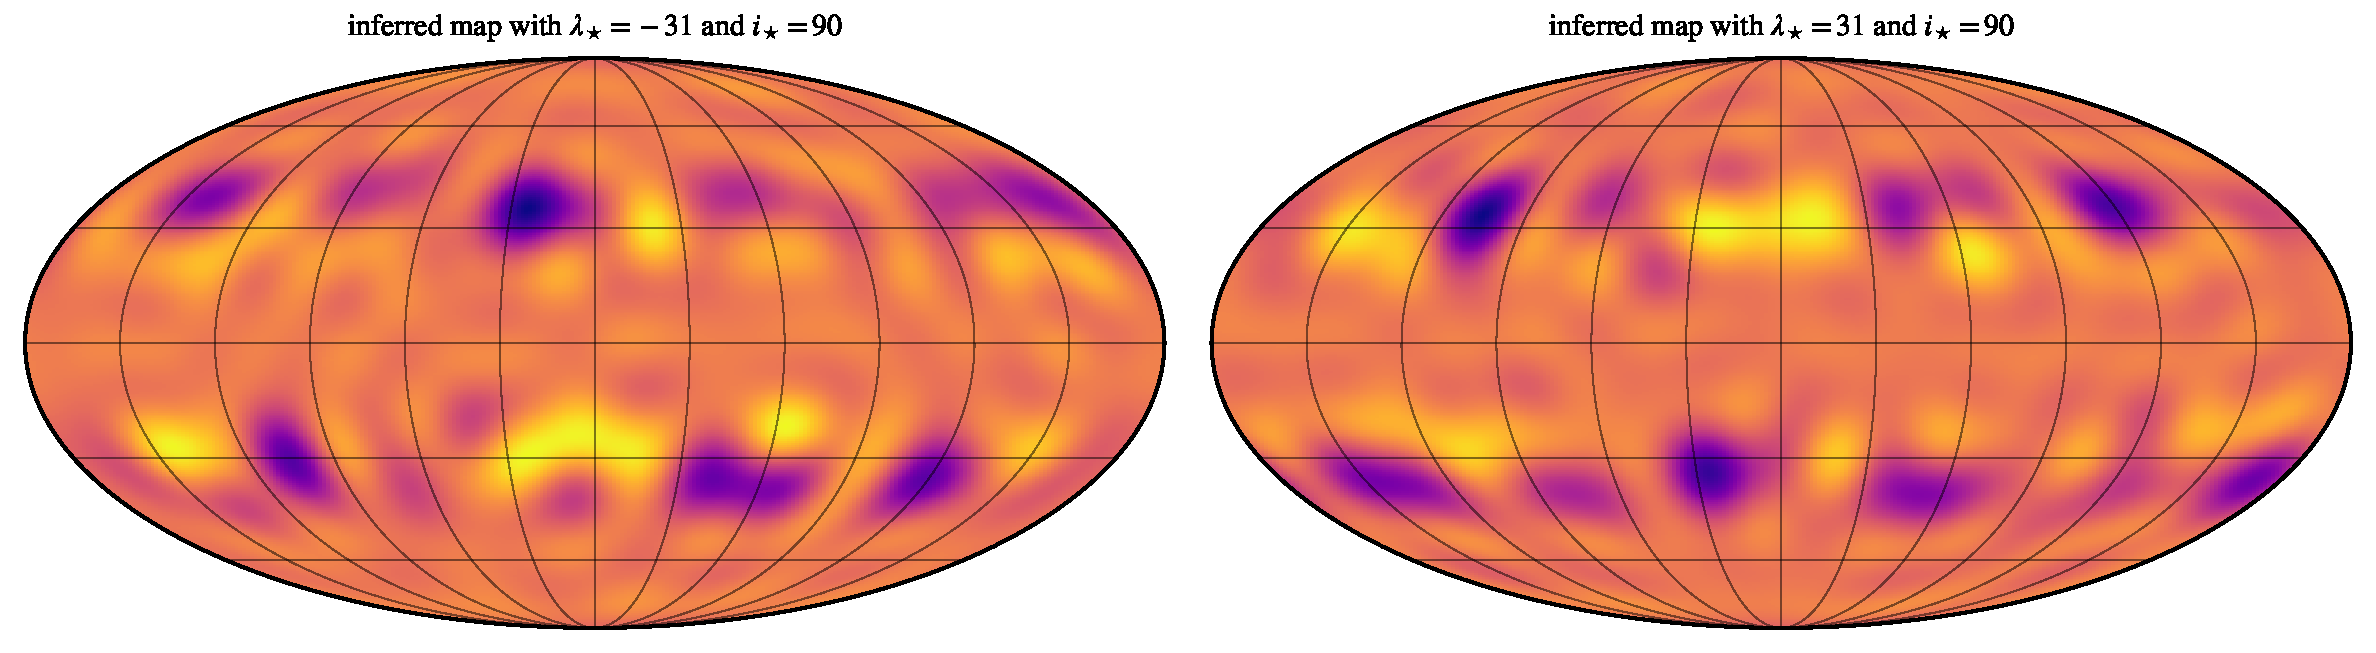
\includegraphics[width=\linewidth]{figures/experiment-1-comparison-inferred-maps.pdf}
        \caption{
            Comparison two inferred stellar surface maps, Left: the inferred stellar surface map, representing the mean of 1000 posterior samples
            but with a changed obliquity to $-\lambda_{\rm inferred}$ and inclination to  $180^\circ-i_{\rm inferred}$. 
            Right: the inferred stellar surface map, representing the mean of 1000 posterior samples
            with an actual inferred obliquity (in this case, $\lambda_{\rm inferred}=\sim 31^\circ$) and inclination $i_{\rm inferred}=90^\circ$.
        }
        \label{fig:experiment-1-inf-map-comparison}
    \end{centering}
\end{figure*}
%

\subsection{Experiment II: evolving surface}
\label{sec:experiment2}

While our primary analysis assumes a static spot distribution across the observational baseline, stellar magnetic activity is 
inherently dynamic. Active regions on stars like TOI-3884 evolve over time, with spots emerging, changing, and disappearing on 
timescales of weeks to months. To explore this time dimension, we developed a preliminary model incorporating temporal 
evolution of the stellar surface features. This experimental approach represents a conceptual extension of our methodology 
rather than a fully validated model, yet it offers compelling insights into the potential for tracking stellar surface evolution 
through transit observations.

By allowing key spot parameters to vary as functions of time between transit epochs, we can begin to probe questions about spot 
lifetimes, differential rotation, and activity cycles—aspects of stellar physics typically requiring long-term monitoring campaigns. 
Our evolving surface model maintains the core framework of our primary analysis while introducing time-dependence to the 
spot distribution through a Gaussian process temporal kernel. This creates a coherent evolution of the surface features that 
respects both the constraints from individual transit events and the physical expectations for how stellar spots behave.
Though this approach requires additional assumptions and computational complexity, initial results suggest that transit light 
curves do contain retrievable information about surface feature evolution. The methodology presented here offers a 
promising avenue for future work, potentially enabling new types of stellar activity studies using already-available 
transit photometry from missions like TESS, Kepler, and the upcoming PLATO mission.

Figures \ref{fig:experiment-2-lc} and \ref{fig:experiment-2-true-maps} showcase the experimental results from our 
evolving surface model. Figure \ref{fig:experiment-2-lc} presents a simulated light curve spanning approximately 150 days, 
demonstrating how stellar rotation and evolving surface features produce complex photometric variations. The black line 
represents the true underlying flux variations, while the blue points with error bars show binned simulated observations. 
This light curve exhibits amplitude variations between approximately 0.87 and 1.12 in relative flux, with complex patterns 
that cannot be explained by simple periodic modulation, indicating the presence of multiple evolving active regions.

Figure \ref{fig:experiment-2-true-maps} complements this time-series data by displaying the corresponding stellar 
surface maps at three representative epochs. Each row presents both a 3D visualization of the stellar hemisphere facing the 
observer (left panels) and a Mollweide projection of the complete stellar surface (right panels). 
These maps reveal the dynamic nature of the spot distribution, with active regions emerging, evolving, and disappearing over time
from top to bottom. Particularly notable is the migration of spots in both latitude and longitude, suggesting potential 
differential rotation, as well as changes in the size and intensity of individual features.

%
\begin{figure*}[hbt!]
    % \script{experiment-1-true-map.py}
    \begin{centering}
        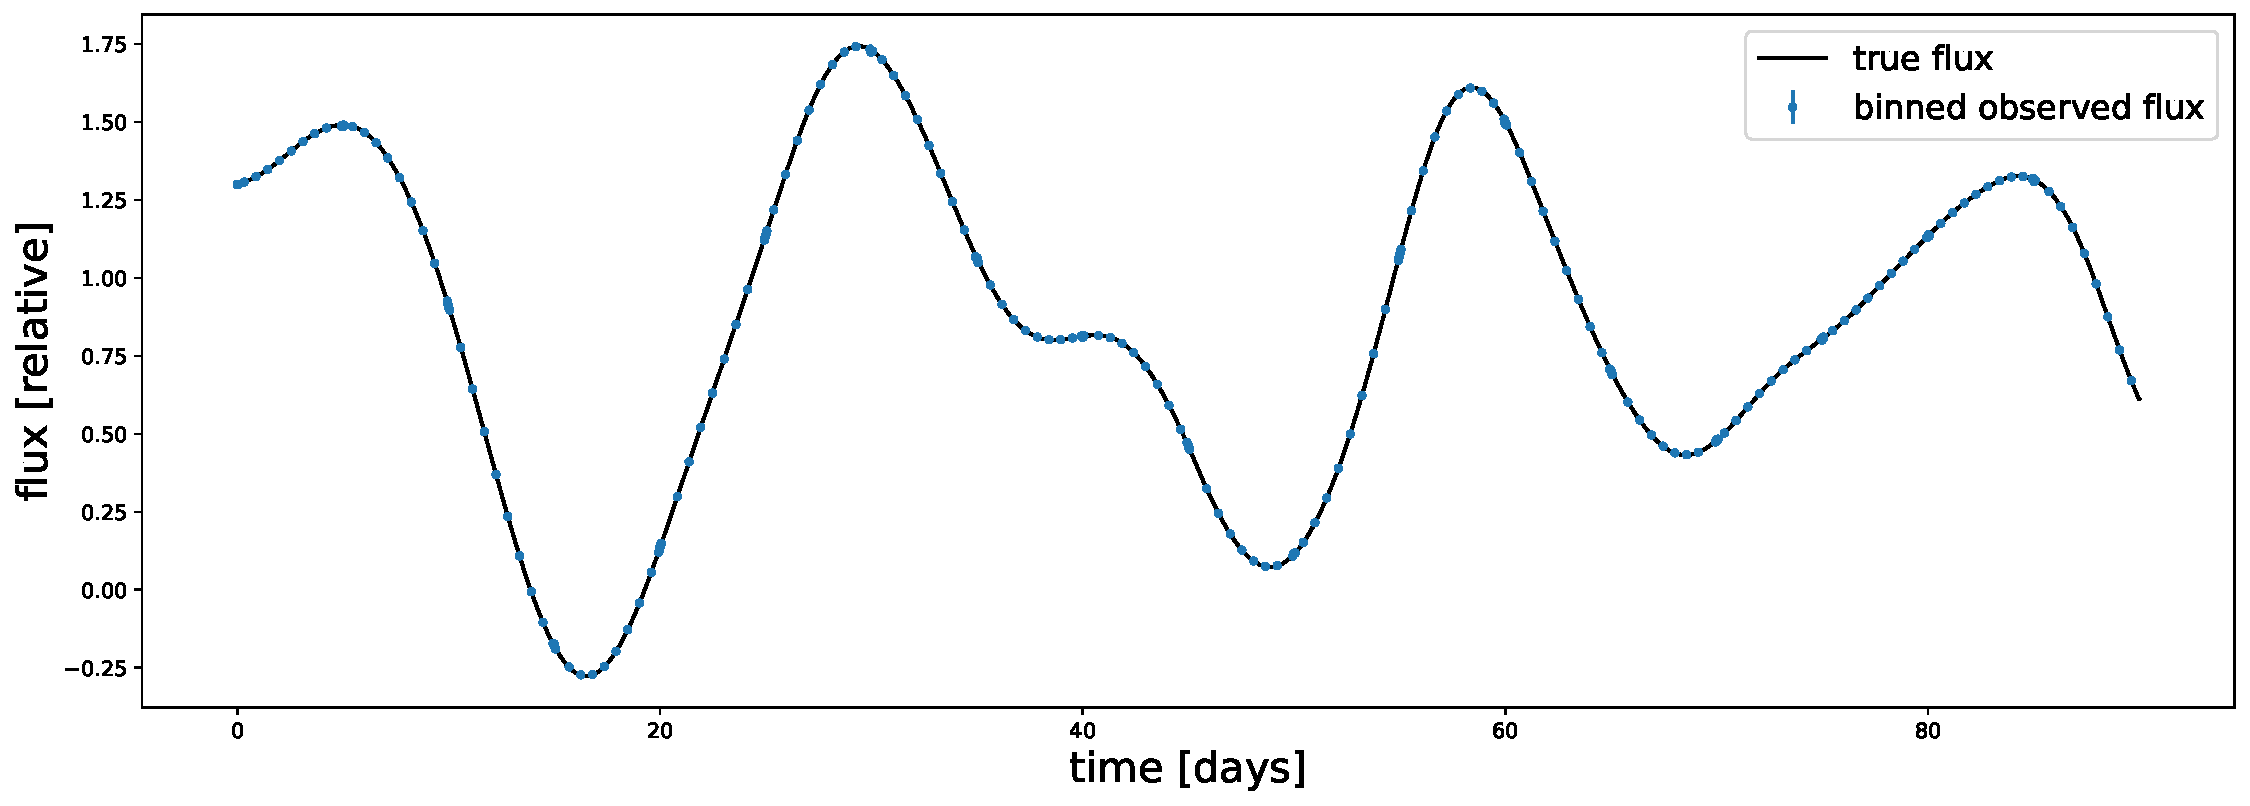
\includegraphics[width=\linewidth]{figures/experiment-2-lc.pdf}
        \caption{
            Simulated light curve from our evolving stellar surface model spanning approximately 150 days. The black line represents 
            the true underlying flux variations, while the blue points with error bars show binned simulated observations. 
            The complex pattern of photometric variability, with amplitude variations between approximately 0.87 and 1.12 in 
            relative flux, reflects the combined effects of stellar rotation and evolving surface features. Note the non-periodic 
            nature of the variations and changing amplitude over time, indicative of multiple active regions evolving at different 
            rates and locations on the stellar surface.}
        \label{fig:experiment-2-lc}
    \end{centering}
\end{figure*}
%
%
\begin{figure}[hbt!]
    % \script{experiment-1-true-map.py}
    \begin{centering}
        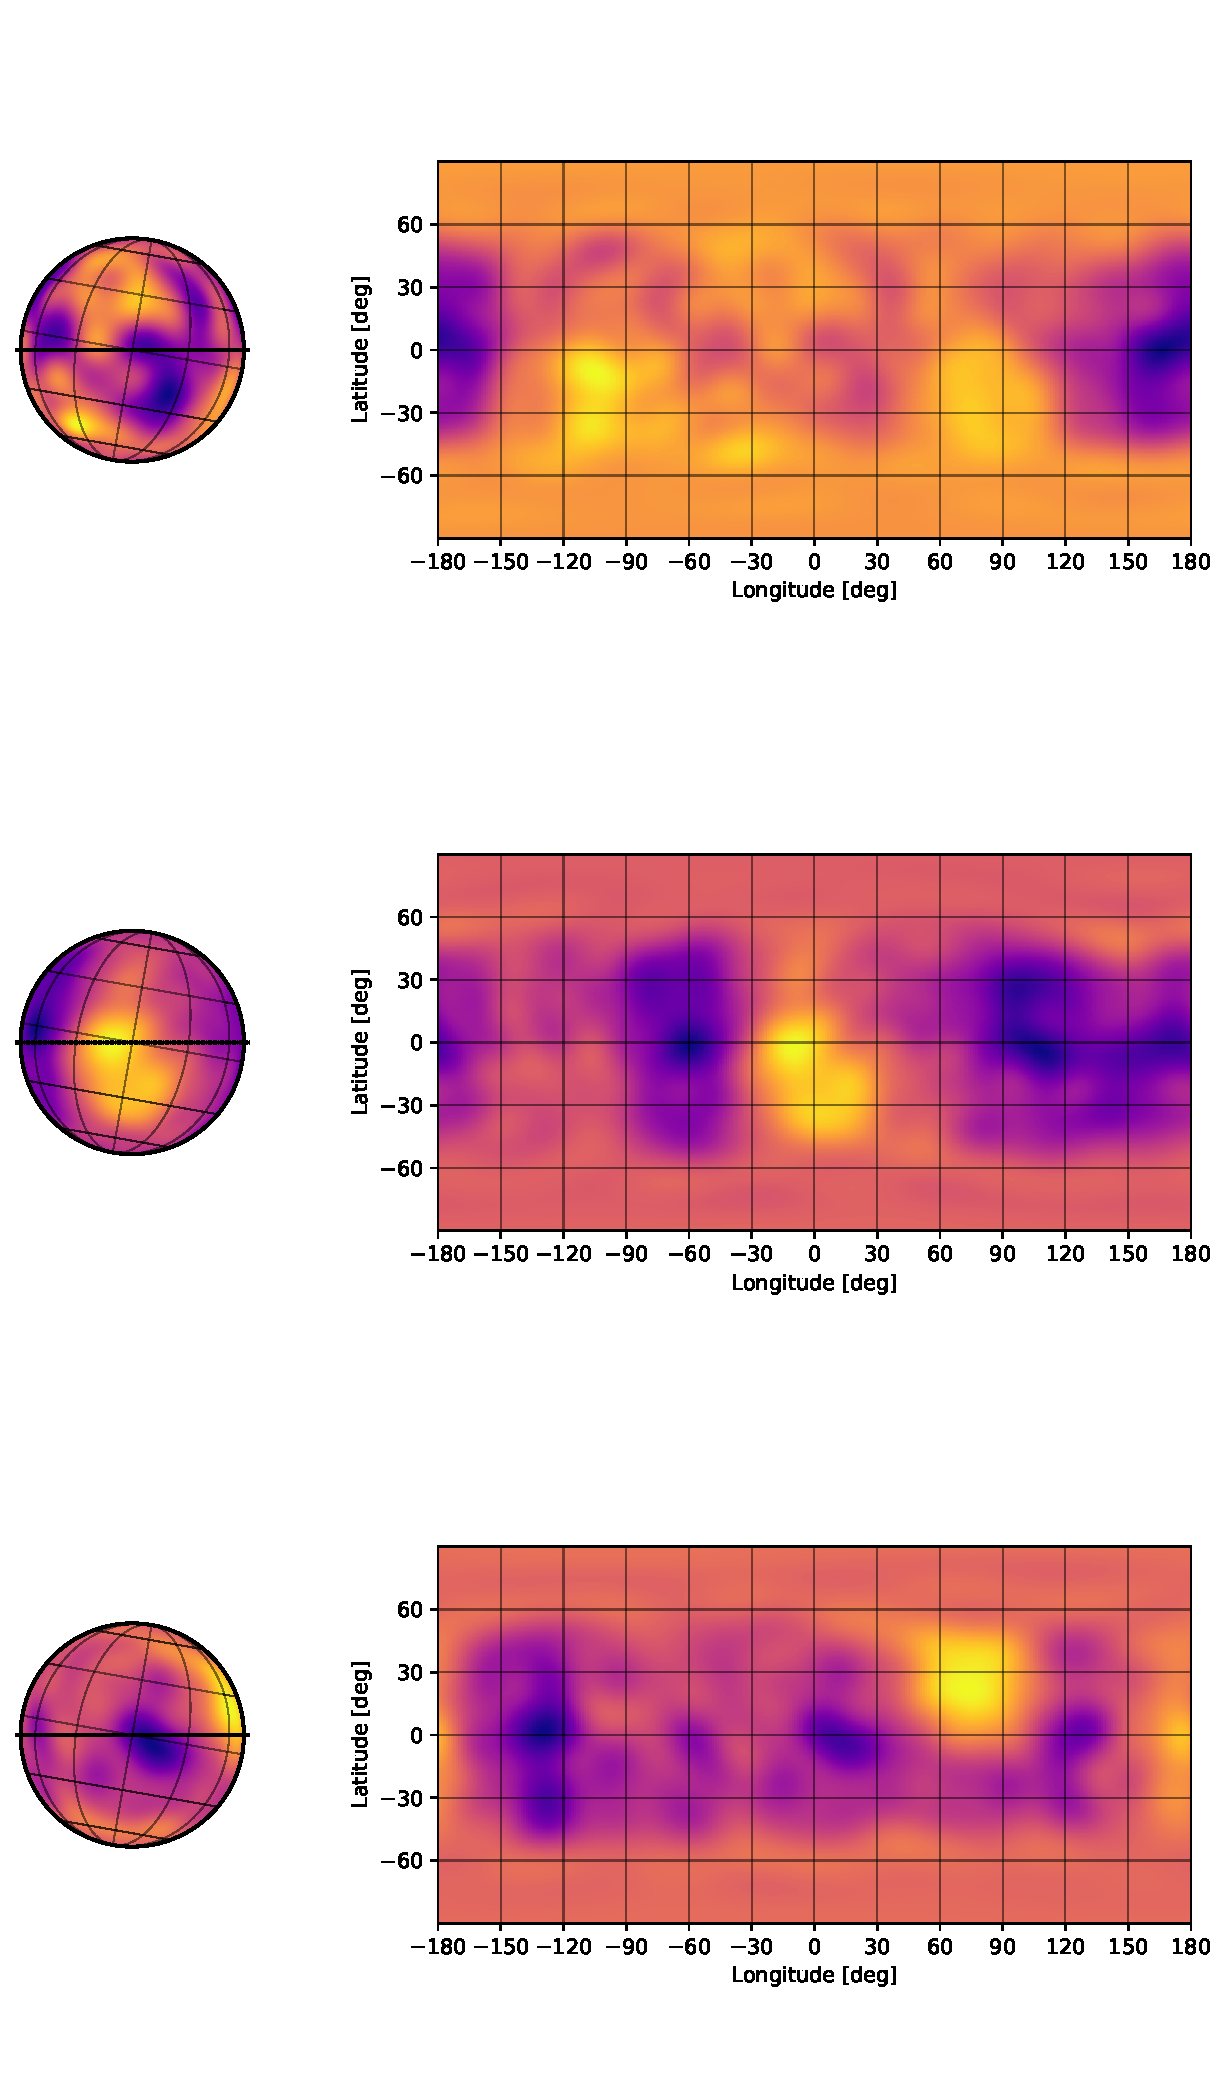
\includegraphics[width=0.86\linewidth]{figures/experiment-2-true-map.pdf}
        \caption{Simulated stellar surface maps at three representative epochs corresponding to the light curve in 
        Figure \ref{fig:experiment-2-lc}. Each row presents both a 3D visualization of the visible stellar hemisphere 
        (left) and a Mollweide projection of the complete surface (right). Dark purple regions indicate cooler spots, while 
        yellow-orange areas represent the warmer photosphere. The maps illustrate the evolution of active regions over time, 
        including changes in spot distribution, emergence of new features, and potential differential rotation effects. 
        The dotted lines on the 3D visualizations indicate the planet's transit path. These surface maps demonstrate how the 
        complex photometric variations in the light curve arise from the dynamic nature of stellar activity patterns.}
        \label{fig:experiment-2-true-maps}
    \end{centering}
\end{figure}
%

Figure \ref{fig:experiment-2-corner} presents the posterior distributions for the key hyperparameters in our spot model. 
The parameters include the spot latitude mean ($\mu_\phi$), latitude variance ($\sigma^2_\phi$), spot contrast parameter 
($\mathbb{c}$), radius ($\mathbb{r}$), and the number of spots ($\mathbb{n}$).
The posterior for spot latitude mean ($\mu_\phi$) is tightly constrained around 30 degrees, consistent with our 
the true value (shown with black lines). We see excellent recovery of the latitude mean, with the true value falling well 
within our posterior distribution and the 1$\sigma$ uncertainty bounds from the simulation aligning well with the width of 
our recovered posterior. The latitude variance ($\sigma^2_\phi$) is centered around 5-6 square degrees, again accurately 
capturing the true value indicated by the black line. Our model successfully recovers this aspect of the spot distribution, 
and our uncertainty estimates appear consistent with the true 1$\sigma$ range. The active latitudes are shown on Firgure \ref{fig:experiment-2-active}.
The radius ($\mathbb{r}$) parameter, which controls the typical size of spot features, is well-constrained at 
approximately 19.5 degrees. Future models will likely improve the recovery of this parameter by incorporating 
multi-wavelength transit observations, which would better constrain the physical extent of surface features by leveraging 
the wavelength-dependent contrast of spots.
The correlation between number of spots ($\mathbb{n}$) and contrast ($\mathbb{c}$) shows 
a well-known degeneracy in spot modeling: as the number of spots increases, the contrast tends to decrease to 
maintain a similar overall flux effect.

%
\begin{figure*}[hbt!]
    % \script{experiment-1-true-map.py}
    \begin{centering}
        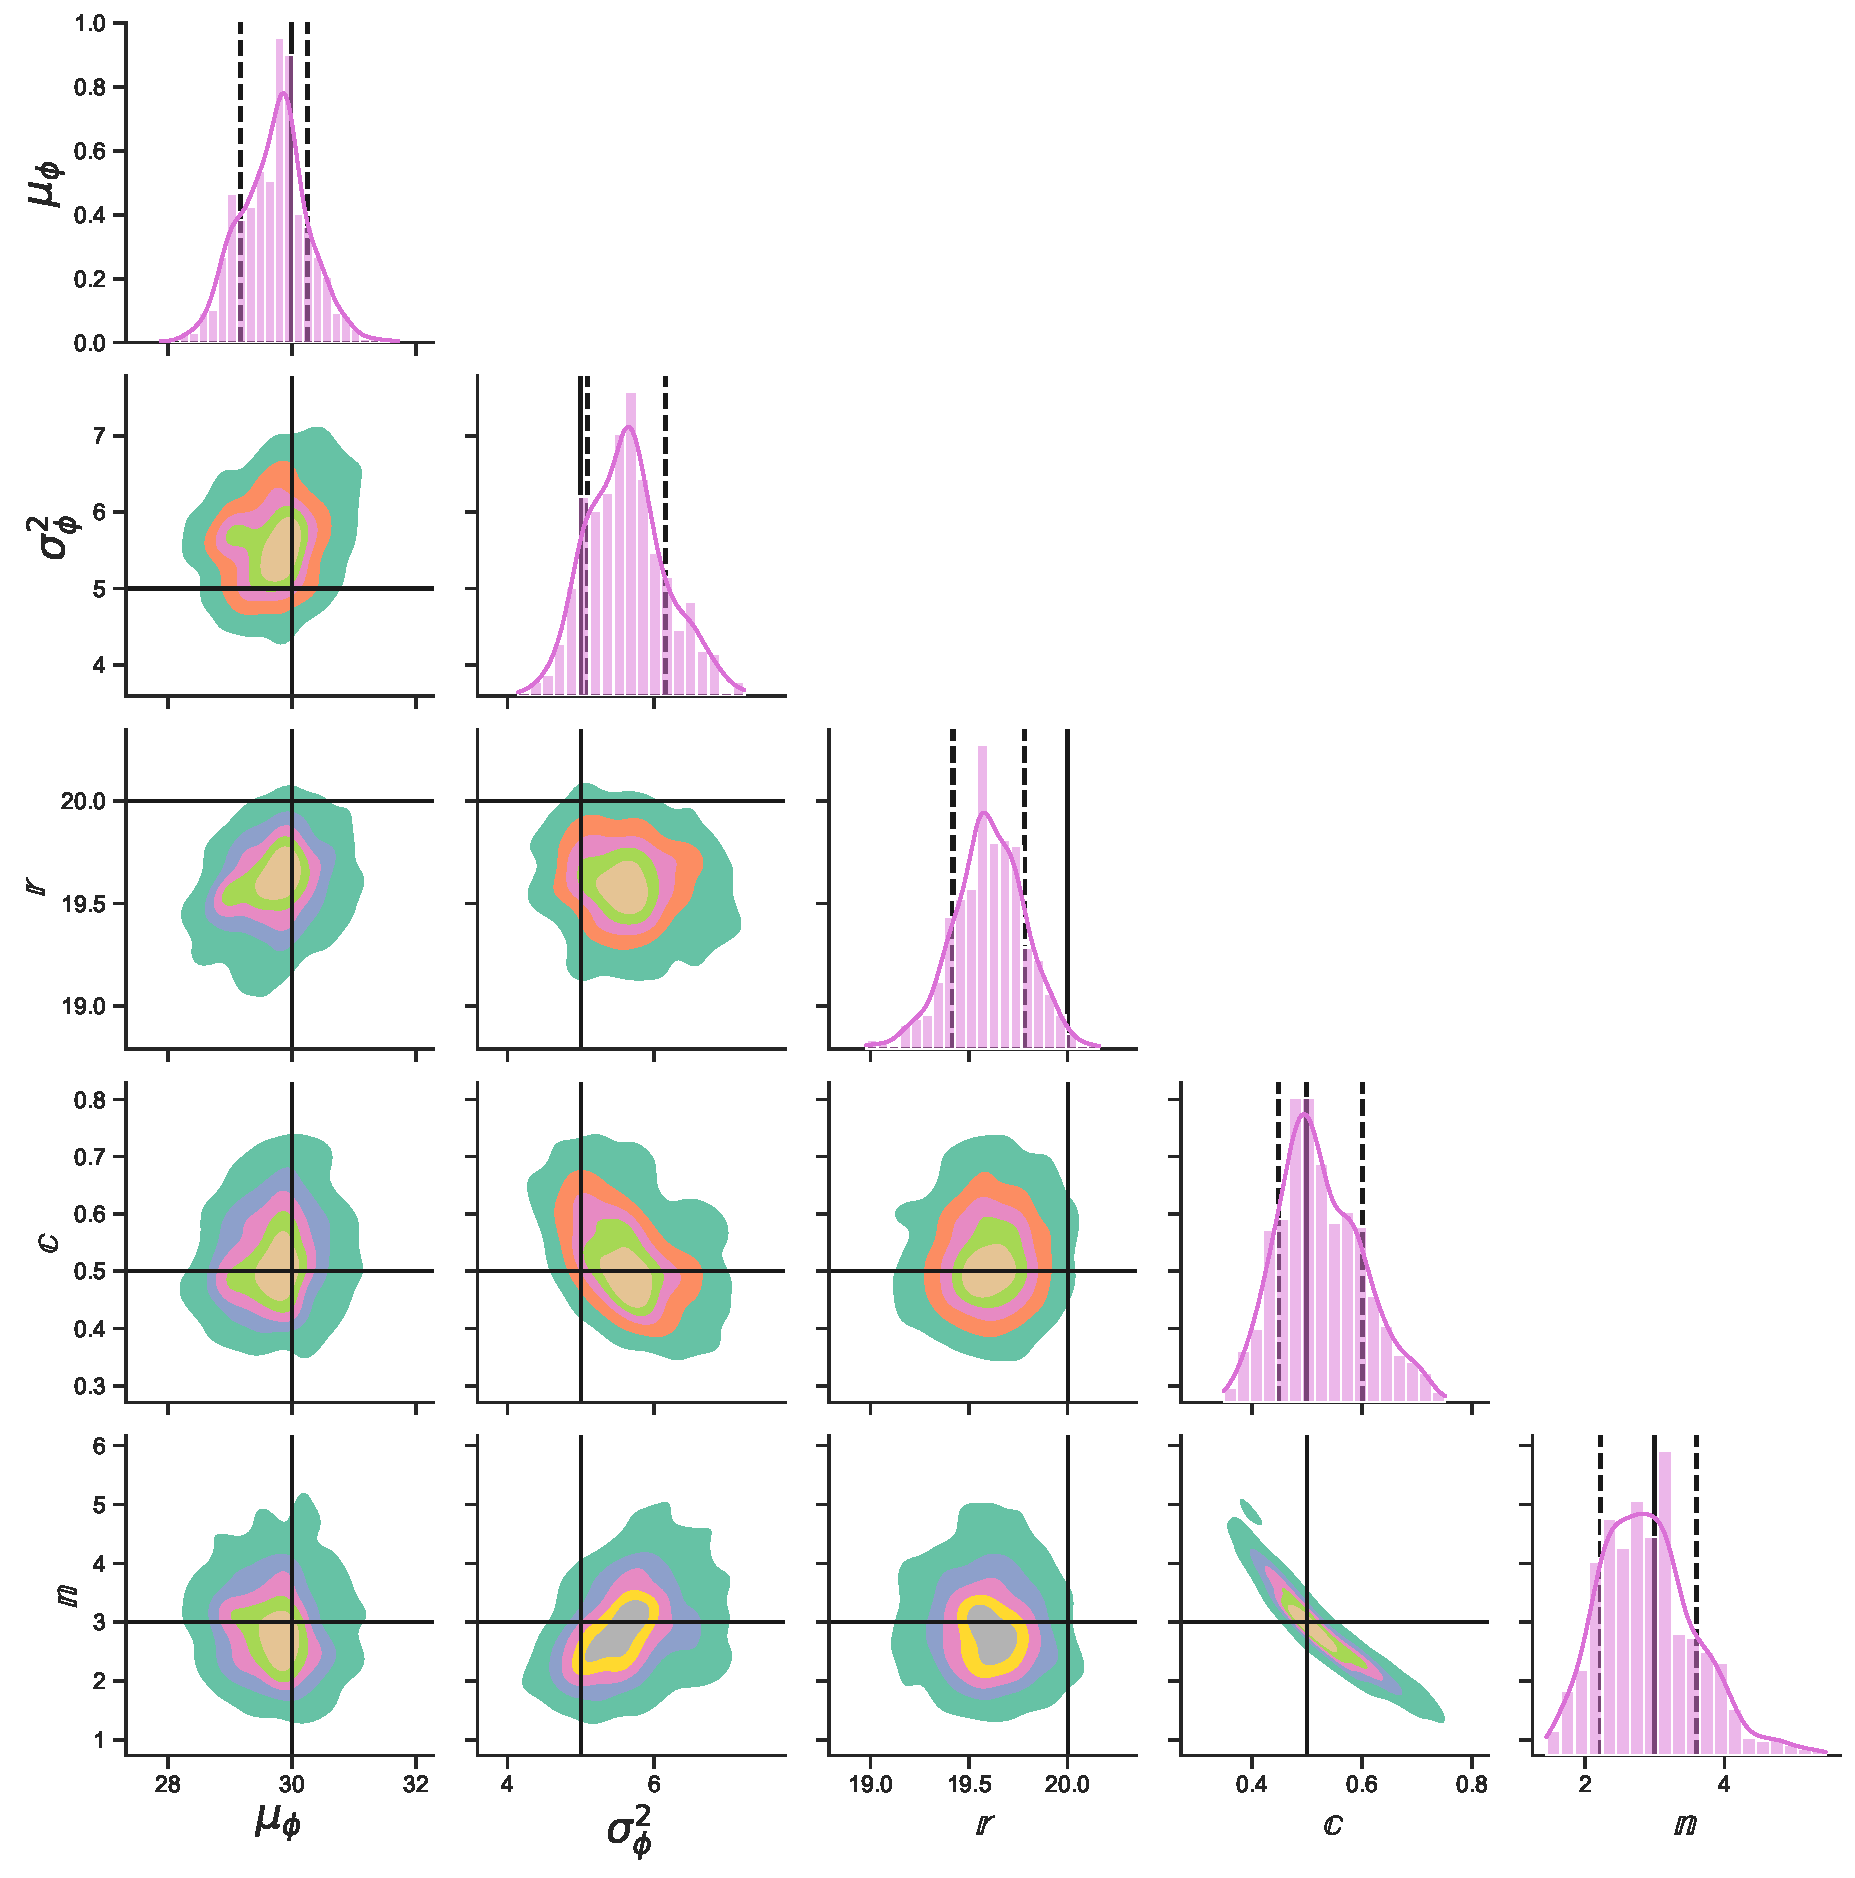
\includegraphics[width=\linewidth]{figures/experiment-2-corner-gps.pdf}
        \caption{Posterior distributions and correlations for key spot model hyperparameters recovered from simulated data. 
        The solid black lines indicate true parameter values used to generate the simulated light curves, while dashed black 
        lines show the $\pm1\sigma$ boundaries. Parameters include spot latitude mean ($\mu_\phi$), latitude variance 
        ($\sigma^2_\phi$), radius ($\mathcal{r}$), spot contrast ($\mathcal{c}$), and number of spots ($n$). 
        The model successfully recovers all parameters within the expected uncertainty ranges.
         Note the correlation between number of spots and contrast, a well-known degeneracy in spot modeling.}
        \label{fig:experiment-2-corner}
    \end{centering}
\end{figure*}
%
%
\begin{figure*}[hbt!]
    % \script{experiment-1-true-map.py}
    \begin{centering}
        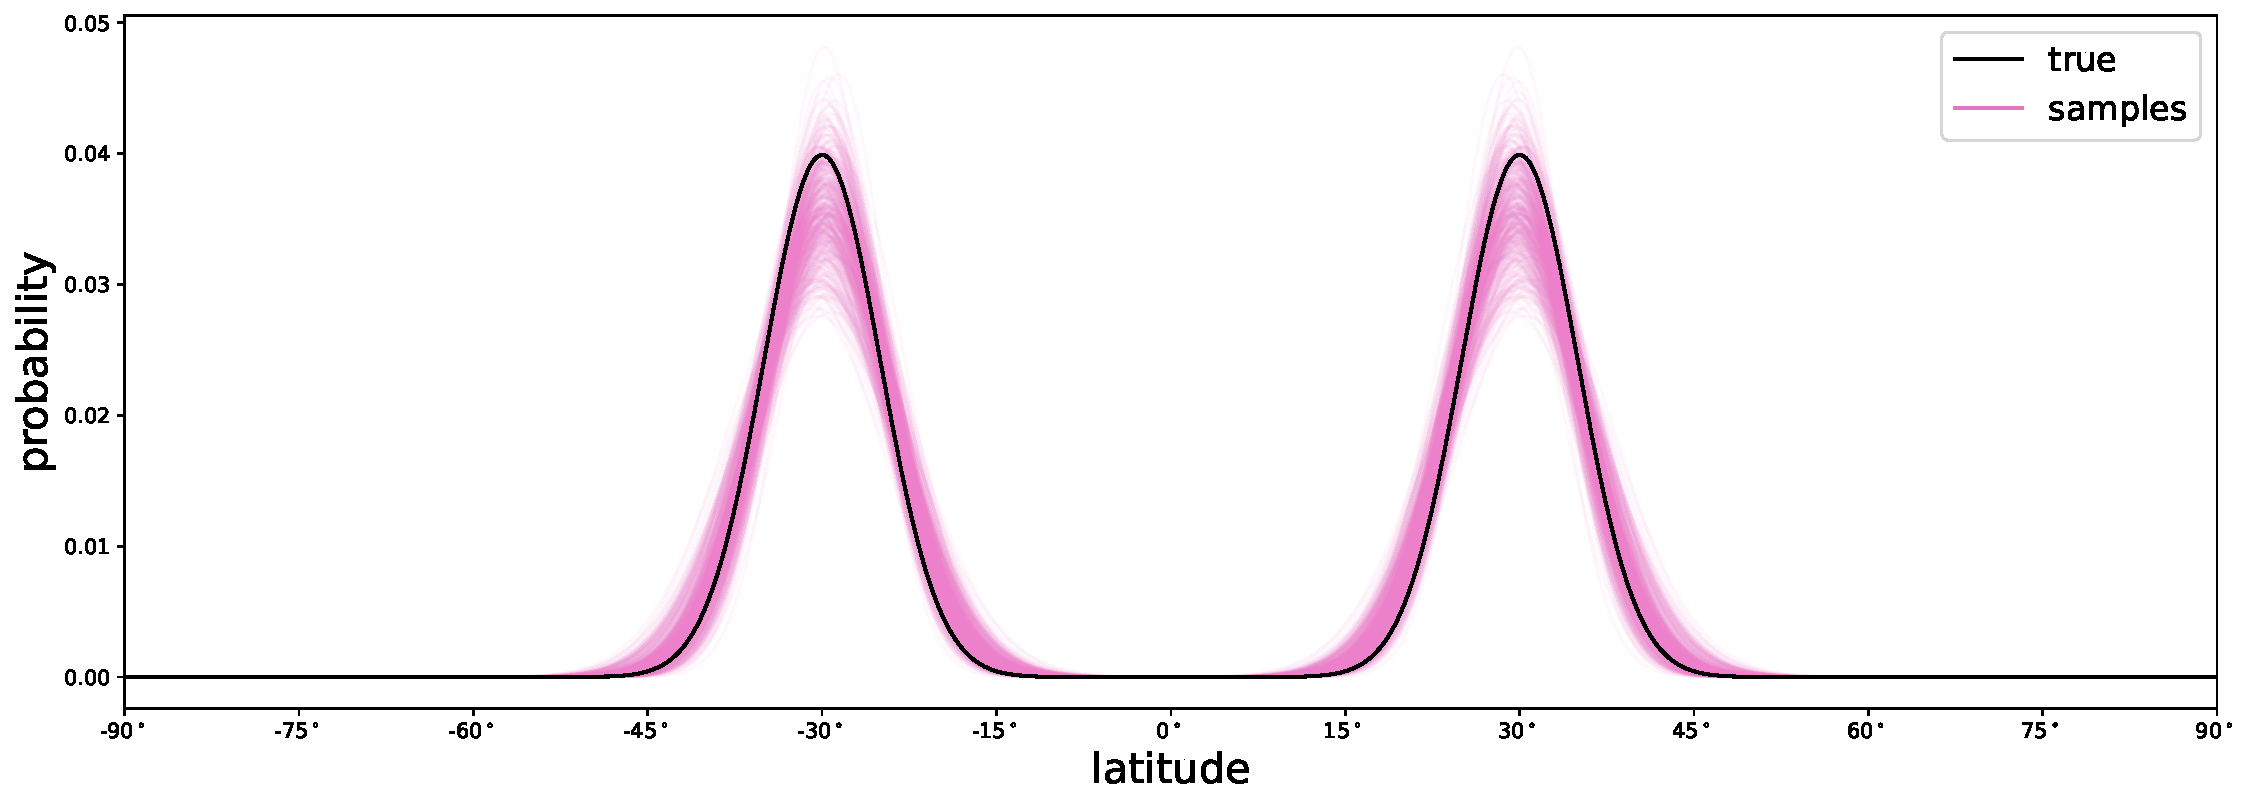
\includegraphics[width=\linewidth]{figures/experiment-2-active-lats.pdf}
        \caption{Posterior probability distribution of spot latitudes for Section \ref{sec:experiment2} just like the Figure 
        \ref{fig:experiment-1-acttive-lats}. The black line shows the true distribution, 
        while the pink lines represent individual posterior samples.}
        \label{fig:experiment-2-active}
    \end{centering}
\end{figure*}
%
Figure \ref{fig:experiment-2-results} presents a comprehensive view of our evolving surface model's ability to reconstruct 
stellar surface features from simulated light curve data. The figure is organized into three key components that demonstrate 
the model's performance at different epochs.
The top portion shows the full simulated light curve (center panel), with three zoomed-in regions highlighting three random consecutive transits 
(top three panels). For each epoch, we compare the observed simulated data points (gray dots) with our model fit (pink line), 
demonstrating excellent agreement between the observations and our reconstruction.
The central portion of the figure displays the true stellar surface maps (left column) alongside our (averaged over 1000 samples) 
inferred reconstructions 
(middle column) at three different epochs, labeled as Map 1, Map 2, and Map 3, where Map 1 evolves to Map 2, which evolves to Map 3. 
Each map is shown as a Mollweide projection with a consistent color scale where dark purple regions indicate cooler spots and 
yellow-orange areas represent the warmer photosphere. The inferred maps show a north-south flip compared to the true maps. 
This hemisphere inversion is a direct manifestation of the inclination-obliquity degeneracy discussed in Section \ref{sec:obl-inc}, 
where transit observations alone cannot distinguish between certain combinations of stellar inclination and obliquity that result 
in mirrored surface feature distributions. Therefore, the resulting obliquity of the star is inferred to be 
$\lambda_\star=30.49^{+0.58}_{-0.49}$ while the true obliquity is $-30^\circ$ (so, the opposite). 
Additionally, the stellar inclination's true 
values is $90^\circ$ while the inferred value is $i_\star=91.36^{+0.33}_{-0.36}$ (close to $180^\circ-i_{\rm true}$).
Despite this expected degeneracy, the inferred maps successfully capture the essential features of the true spot distribution, 
including the number, approximate size, and longitudinal positioning of major active regions. This is particularly evident in 
Map 3, where the model correctly identifies a prominent high-latitude bright region, though it places it in the opposite 
hemisphere.
The right column shows the corresponding light curve sections for each map epoch, further illustrating how well our model 
reproduces the observed flux variations despite the hemisphere ambiguity. The bottom panel presents the complete light curve 
with vertical lines marking the times corresponding to the three maps, contextualizing how the surface features evolve over the 
full observational baseline.
This figure demonstrates that while inherent degeneracies prevent unique determination of the absolute spot latitudes from 
transit data alone, our model can nevertheless recover detailed and physically meaningful information about the evolution of 
stellar surface features.
%
\begin{figure*}[hbt!]
    % \script{experiment-1-true-map.py}
    \begin{centering}
        \includegraphics[width=\linewidth]{figures/experiment-2-results.pdf}
        \caption{Comparison between true and inferred stellar surface maps from our evolving surface model using simulated data. 
        Top: Simulated light curve (center) with three transit epochs (above). Middle: True stellar surface maps (left column) 
        and our inferred reconstructions averaged over 1000 samples (middle column) at three epochs. Bottom: Full light curve 
        with vertical lines marking the three mapped epochs. Note the north-south inversion in the inferred maps compared to 
        the true maps, demonstrating the inclination-obliquity degeneracy discussed in Section \ref{sec:obl-inc}. 
        Despite this expected degeneracy, our model successfully recovers the number, approximate size, and longitudinal 
        positioning of major active regions, with excellent agreement between the model light curve (red line) and simulated 
        observations (gray points).}
        \label{fig:experiment-2-results}
    \end{centering}
\end{figure*}
%

\section{The Case of TOI-3884}
\label{sec:toi3884}
In this section, we present the results of the model application on TESS light curves of TOI-3884. While TOI-3884 presents a relatively straightforward case, 
it serves as an excellent testbed for demonstrating the capabilities and functionality of our model. By applying our model to TOI-3884, we aim to validate 
its performance on a well-understood system, highlight its ability to extract meaningful information from a real light curve, 
and lay the groundwork for more complex analyses by establishing a baseline of performance.

TOI-3884 (also known as TIC 86263325) was observed by the TESS mission across multiple sectors. The star was monitored for 81 days over a 765-day span, 
using both 30-minute and 2-minute cadences. While Gaia observations show that the TESS aperture for this target isn't significantly contaminated by nearby stars, 
the light curve reveals several transiting spot crossings, indicating stellar activity. Various light curve products were generated for TOI-3884, 
including Simple Aperture Photometry (SAP) 
from the TESS Science Processing Operations Centre and Kepler Spline SAP (KSPSAP) from the Quick-Look Pipeline \citep{Huang2020}. 

TESS revisited TOI-3884 in Sectors 46 and 49, spanning parts of late 2021 and early 2022, using short-cadence observations with 2-minute exposures. 
We used the \texttt{lightkurve} package \citep{lightkurve} to process data from all three sectors, applying strict quality control measures to 
the Pre-search Data Conditioning Simple Aperture Photometry \citep{jenkins2016}.

\begin{figure*}[hbt!]
    % \script{experiment-1-true-map.py}
    \begin{centering}
        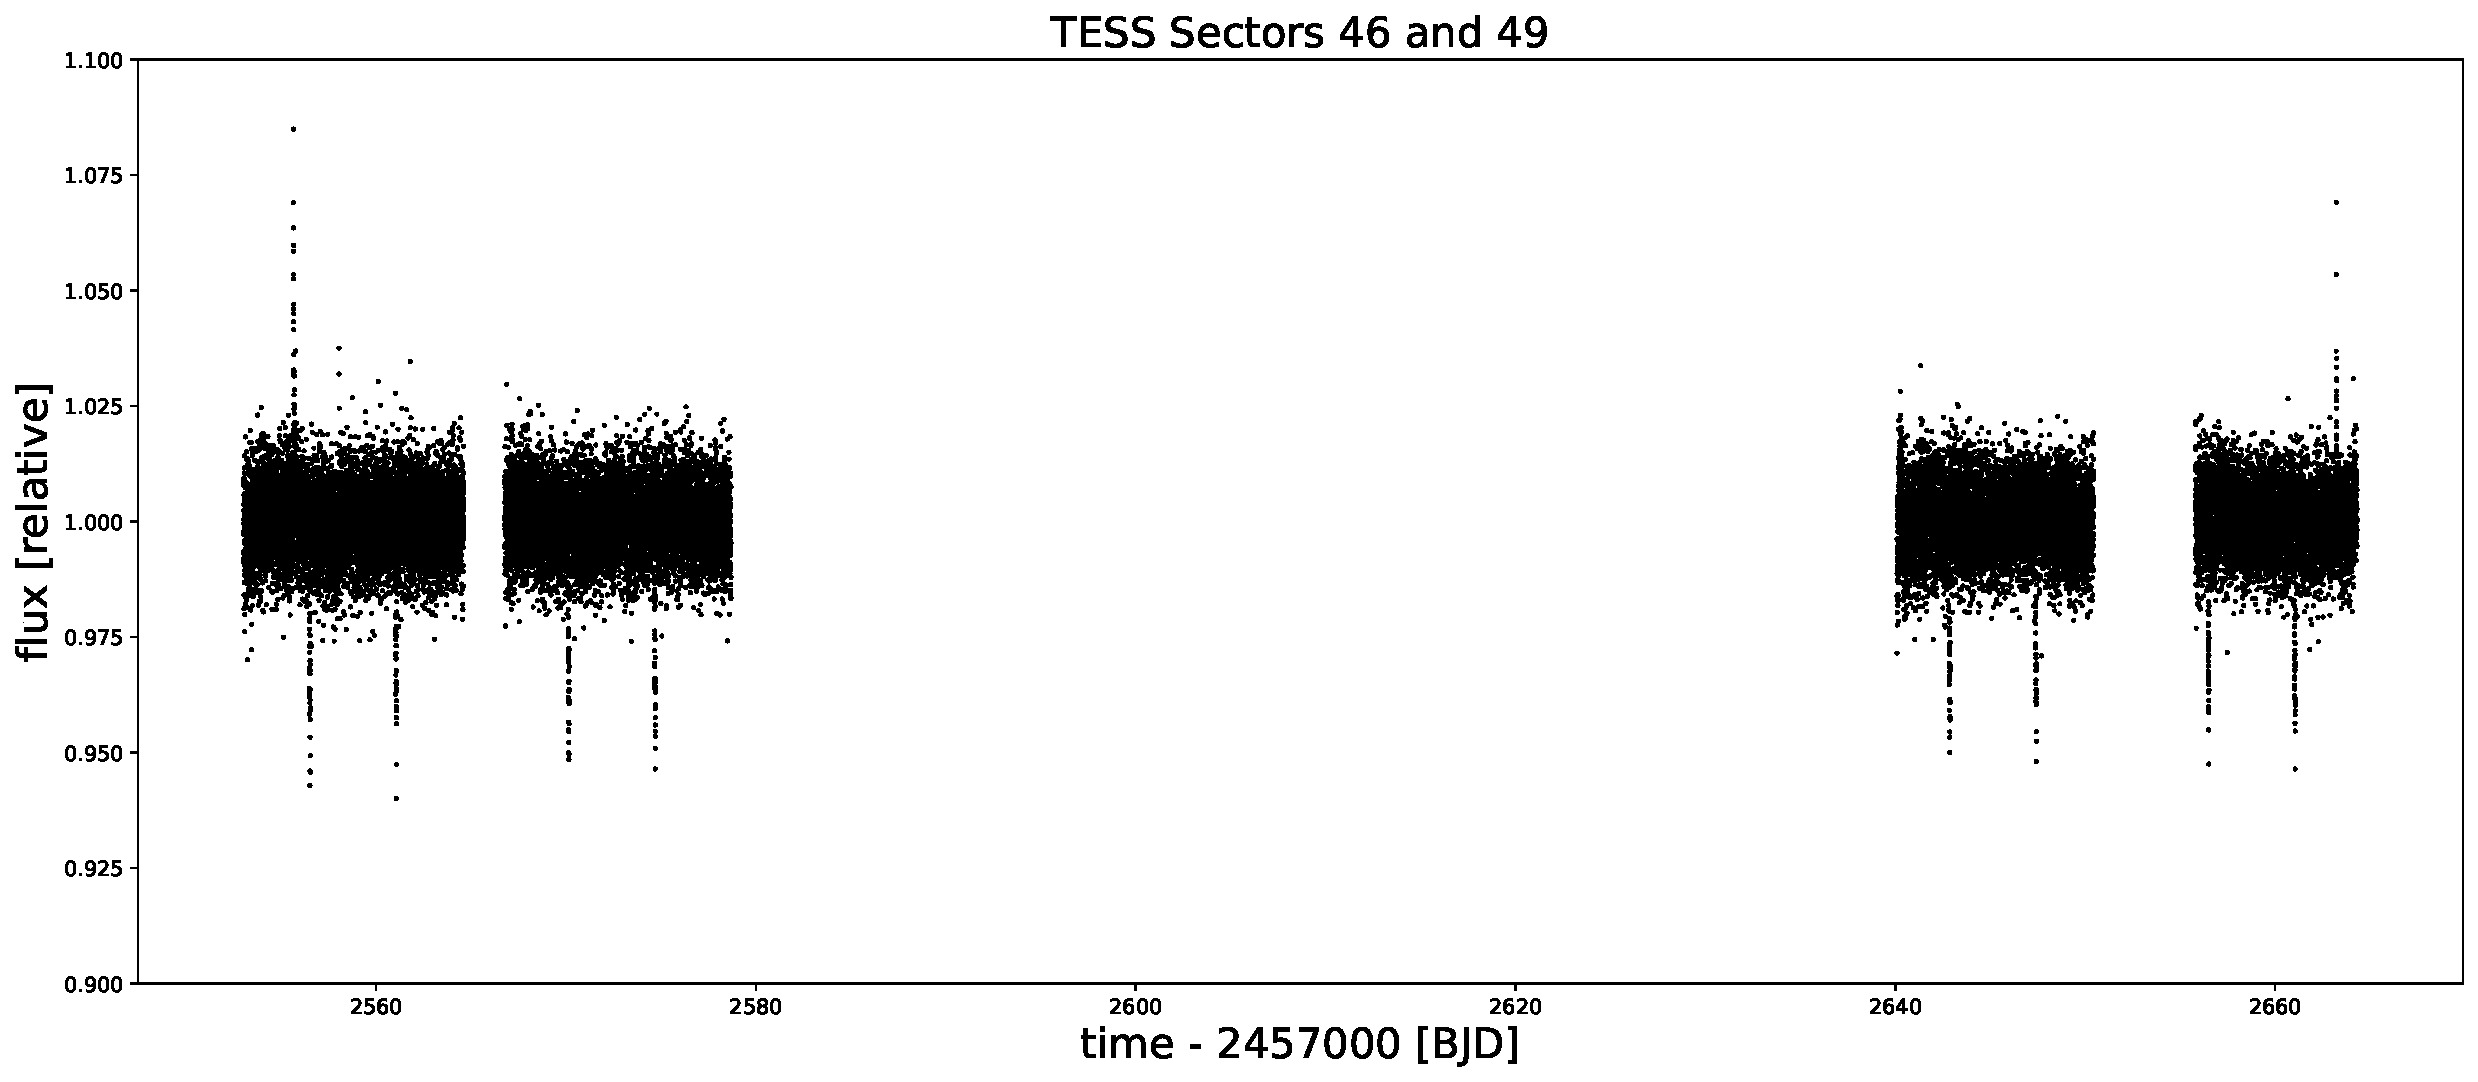
\includegraphics[width=\linewidth]{figures/toi3884-lc.pdf}
        \caption{
            Short 2-minute cadence of the TESS Sectors 46 and 49. 
            Both sets of light curves use the PDCSAP flux.
        }
        \label{fig:toi-3884-pdscap-lc}
    \end{centering}
\end{figure*}

\subsection{Priors for TOI-3884 and TOI-3384 b}

Below, we detail each parameter's prior distribution. We denote the initial values taken from the discovery work of TOI-3884 as 
$\_\rm transit$ taken from \cite{Almenara2022} and the values from the RV observations as $\_\rm RV$ taken from \cite{Libby-Roberts2023}.

The impact parameter $b$ follows a uniform distribution between $-b_{\text{max}}$ and $b_{\text{max}}$, 
where $b_{\text{max}} = R_{\star}/a$ represents the ratio of the stellar radius to the semi-major axis. 
This prior encompasses all possible transit geometries, including grazing transits: $b \sim \mathcal{U}(-b_{\text{max}}, 
b_{\text{max}})$.

The orbital eccentricity $e$ is constrained to physically meaningful values with a uniform prior between 0 (circular orbit) and 1 (parabolic orbit): 
$e \sim \mathcal{U}(0, 1)$.

For the orbital period $P_{\text{orb}}$, we use a tight uniform prior on a scaling factor $f_{P_{\text{orb}}}$ around the known value: 
$f_{P_{\text{orb}}} \sim \mathcal{U}(0.99, 1.01)$, with the actual period derived as $P_{\text{orb}} = P_{\text{orb,transit}} \cdot f_{P_{\text{orb}}}$. 
This allows for small adjustments to the period while maintaining consistency with observed transits.

Similarly, the mid-transit time $t_0$ is parameterized through a scaling factor $f_{t_0} \sim \mathcal{U}(0.9, 1.1)$, 
with the actual time calculated as $t_0 = t_{0,\text{transit}} + P_{\text{orb,transit}} \cdot (f_{t_0} - 1)$. 
This formulation permits the mid-transit time to vary within approximately $\pm10\%$ of the orbital period from the initial estimate.

The planet radius is parameterized in log space with a uniform prior that allows it to vary between half and twice the 
initially estimated value: $\ln(R_p) \sim \mathcal{U}(\ln(R_{p,\text{transit}}/2), \ln(2 \cdot R_{p,\text{transit}}))$.

The orientation of the orbital angular momentum is parameterized through $w_x$ and $w_y$, which follow standard normal 
distributions: $w_x, w_y \sim \mathcal{N}(0, 1)$. 
This provides a uniform distribution over the unit sphere when properly transformed to three dimensions.

The stellar position parameters $\tilde{x}_{\star}$, $\tilde{y}_{\star}$, and $\tilde{z}_{\star}$ similarly follow standard normal 
distributions: $\tilde{x}_{\star}$, $\tilde{y}_{\star},\tilde{z}_{\star} \sim \mathcal{N}(0, 1)$, allowing for uncertainty in the precise position 
of the star.

The limb darkening coefficients for a quadratic limb darkening law are given uniform priors: 
$u_1 \sim \mathcal{U}(0, 0.5)$ and $u_2 \sim \mathcal{U}(0, 0.2)$. These ranges are consistent with typical values 
for main-sequence stars.

The stellar rotation period $P_{\text{rot}}$ is parameterized as a multiple of the estimated 
value: $f_{P_{\text{rot}}} \sim \mathcal{U}(0.2, 1.8)$ with $P_{\text{rot}} = f_{P_{\text{rot}}} 
\cdot 10$, allowing the rotation period to vary between 20\% and 180\% of the initial estimate. This translates to the uniform 
distribution from 2 to 18 days.

The stellar mass follows a log-normal distribution derived from density measurements: 
$\ln(M_{\star}) \sim \mathcal{N}(\ln(\rho_{\rm RV} / \rho_{\odot}), \sigma_{\rho_{\rm RV}} / \rho_{\rm RV})$. 
This prior incorporates observational constraints on the stellar density while properly accounting for the uncertainty.
The radius of the star stays fixed at 1 $R_\odot$.

For the Gaussian Process (GP) kernel parameters modeling stellar activity, we employ uniform priors: the radius of spots 
$\mathbb{r} \sim \mathcal{U}(10.0, 60.0)$, the contrast $\mathbb{c} \sim \mathcal{U}(0.01, 0.9)$, 
the number of spots $\mathbb{n} \sim \mathcal{U}(0.1, 10.0)$, the mean of the latitude distribution $\mu_\phi \sim \mathcal{U}(0.1, 80.0)$, 
and the variance of the latitude distribution $\sigma^2_\phi \sim \mathcal{U}(0.1, 20.0)$.

All parameters constrained to specific ranges are implemented using logit/inverse-logit transformations with appropriate 
Jacobian adjustments in the log-probability calculations to maintain proper probability distributions.

\subsection{Addressing Multimodality with Parallel Tempering}

The posterior distribution of our model exhibits significant multimodality, presenting substantial challenges for 
conventional sampling methods. This multimodality arises from several sources inherent to transit modeling. 
First, the degeneracy between impact parameter and planet radius creates multiple regions of high posterior probability. 
Second, the periodic nature of orbital elements introduces symmetries in the likelihood landscape, particularly when stellar 
activity signals interact with planetary transit signatures. Third, the parameterization of stellar rotation and activity through 
our model introduces additional complexity with multiple viable configurations that can explain the observed data equally well.

Standard Markov Chain Monte Carlo (MCMC) methods such as Ensemble Sampling (e.g., \texttt{emcee} \cite{emcee}) or Hamiltonian Monte Carlo (HMC; \cite{Hoffman2011}) struggle 
in this multimodal landscape. Ensemble samplers can become trapped in local modes, failing to explore the full posterior 
distribution even with large numbers of walkers. This "mode-trapping" problem is particularly severe in our high-dimensional 
parameter space, where narrow connecting pathways between modes create bottlenecks for efficient sampling. Similarly, 
HMC methods, while excellent for exploring complicated geometries within a single mode, typically fail to transition between 
widely separated modes due to the momentum-based dynamics that govern their exploration.

To overcome these limitations, we utilized Parallel Tempering (PT), also known as replica exchange MCMC. 
This method simultaneously runs multiple MCMC chains at different "temperatures," where temperature controls the 
degree to which the posterior is flattened. At high temperatures, the likelihood is down-weighted, allowing chains to 
move more freely across the parameter space and easily traverse valleys between modes. At the lowest temperature 
($T=1$), the chain samples from the true posterior of interest.

The key innovation in PT is the periodic exchange of states between chains at adjacent temperatures. 
These exchanges allow configurations discovered at high temperatures to propagate down to the cold chain, 
effectively enabling jumps between modes that would be extremely rare in standard MCMC. We used the implementation
of PT in \texttt{ptemcee} \citep{ptemcee}. \texttt{ptemcee} handles these exchanges using the Metropolis criterion:

\begin{equation}
    \label{eq:ptemcee}
    P_{\rm exchange} = \min\left(1, \exp\left[\left(\frac{1}{T_i} - \frac{1}{T_j}\right)\right.\right.\left.\left.\left(\ln \mathcal{L}(\theta_j) - \ln \mathcal{L}(\theta_i)\right)\right]\right)
\end{equation}

where $T_i$ and $T_j$ are the temperatures of adjacent chains, and $\theta_i$ and $\theta_j$ are their respective states.
Our implementation used a ladder of 8 temperatures geometrically spaced between $T=1$ and $T=\infty$, with exchange attempts proposed 
every 10 iterations. To validate adequate sampling across modes, we monitored the exchange acceptance rates between adjacent 
temperature levels, aiming for rates between 10\% and 40\%.

\subsection{Results}
The full posterior distributions for all model parameters are summarized in Table \ref{tab:ResultsT0i3884}. Here, we highlight the 
most significant results.

The spot model strongly favors a high-latitude feature with an angular radius of $\mathbb{r} = 26.77^{+9.7}_{-8.7}$ degrees, 
covering approximately 2.5-10\% of the stellar surface. 

Figure \ref{fig:spot_parameters} presents the posterior distributions and correlations of the key parameters in our spot model. 
Our analysis strongly favors a high-latitude spot configuration with the spot center located at $\mu_{\phi} = {75.3}^{+3.7}_{-4.2}$ 
degrees, indicating a near-polar feature. The spot contrast parameter $\mathbb{c} = 0.049^{+0.028}_{-0.013}$ corresponds to a 
moderate temperature difference between the spot and surrounding photosphere, consistent with typical values observed on active M 
dwarfs. The angular variance in longitude $\sigma^2_{\phi}$ shows bimodality, with peaks at approximately $5^{\circ}$ 
and $15^{\circ}$, indicating two distinct possible spot configurations with different latitudinal spreads. 
The close correlation between stellar inclination and spot latitude reflects the geometric constraints imposed by the transit 
observations. Collectively, these parameters paint a picture of TOI-3884 as an active star with significant polar spotting.

\begin{figure*}[hbt!]
    \centering
    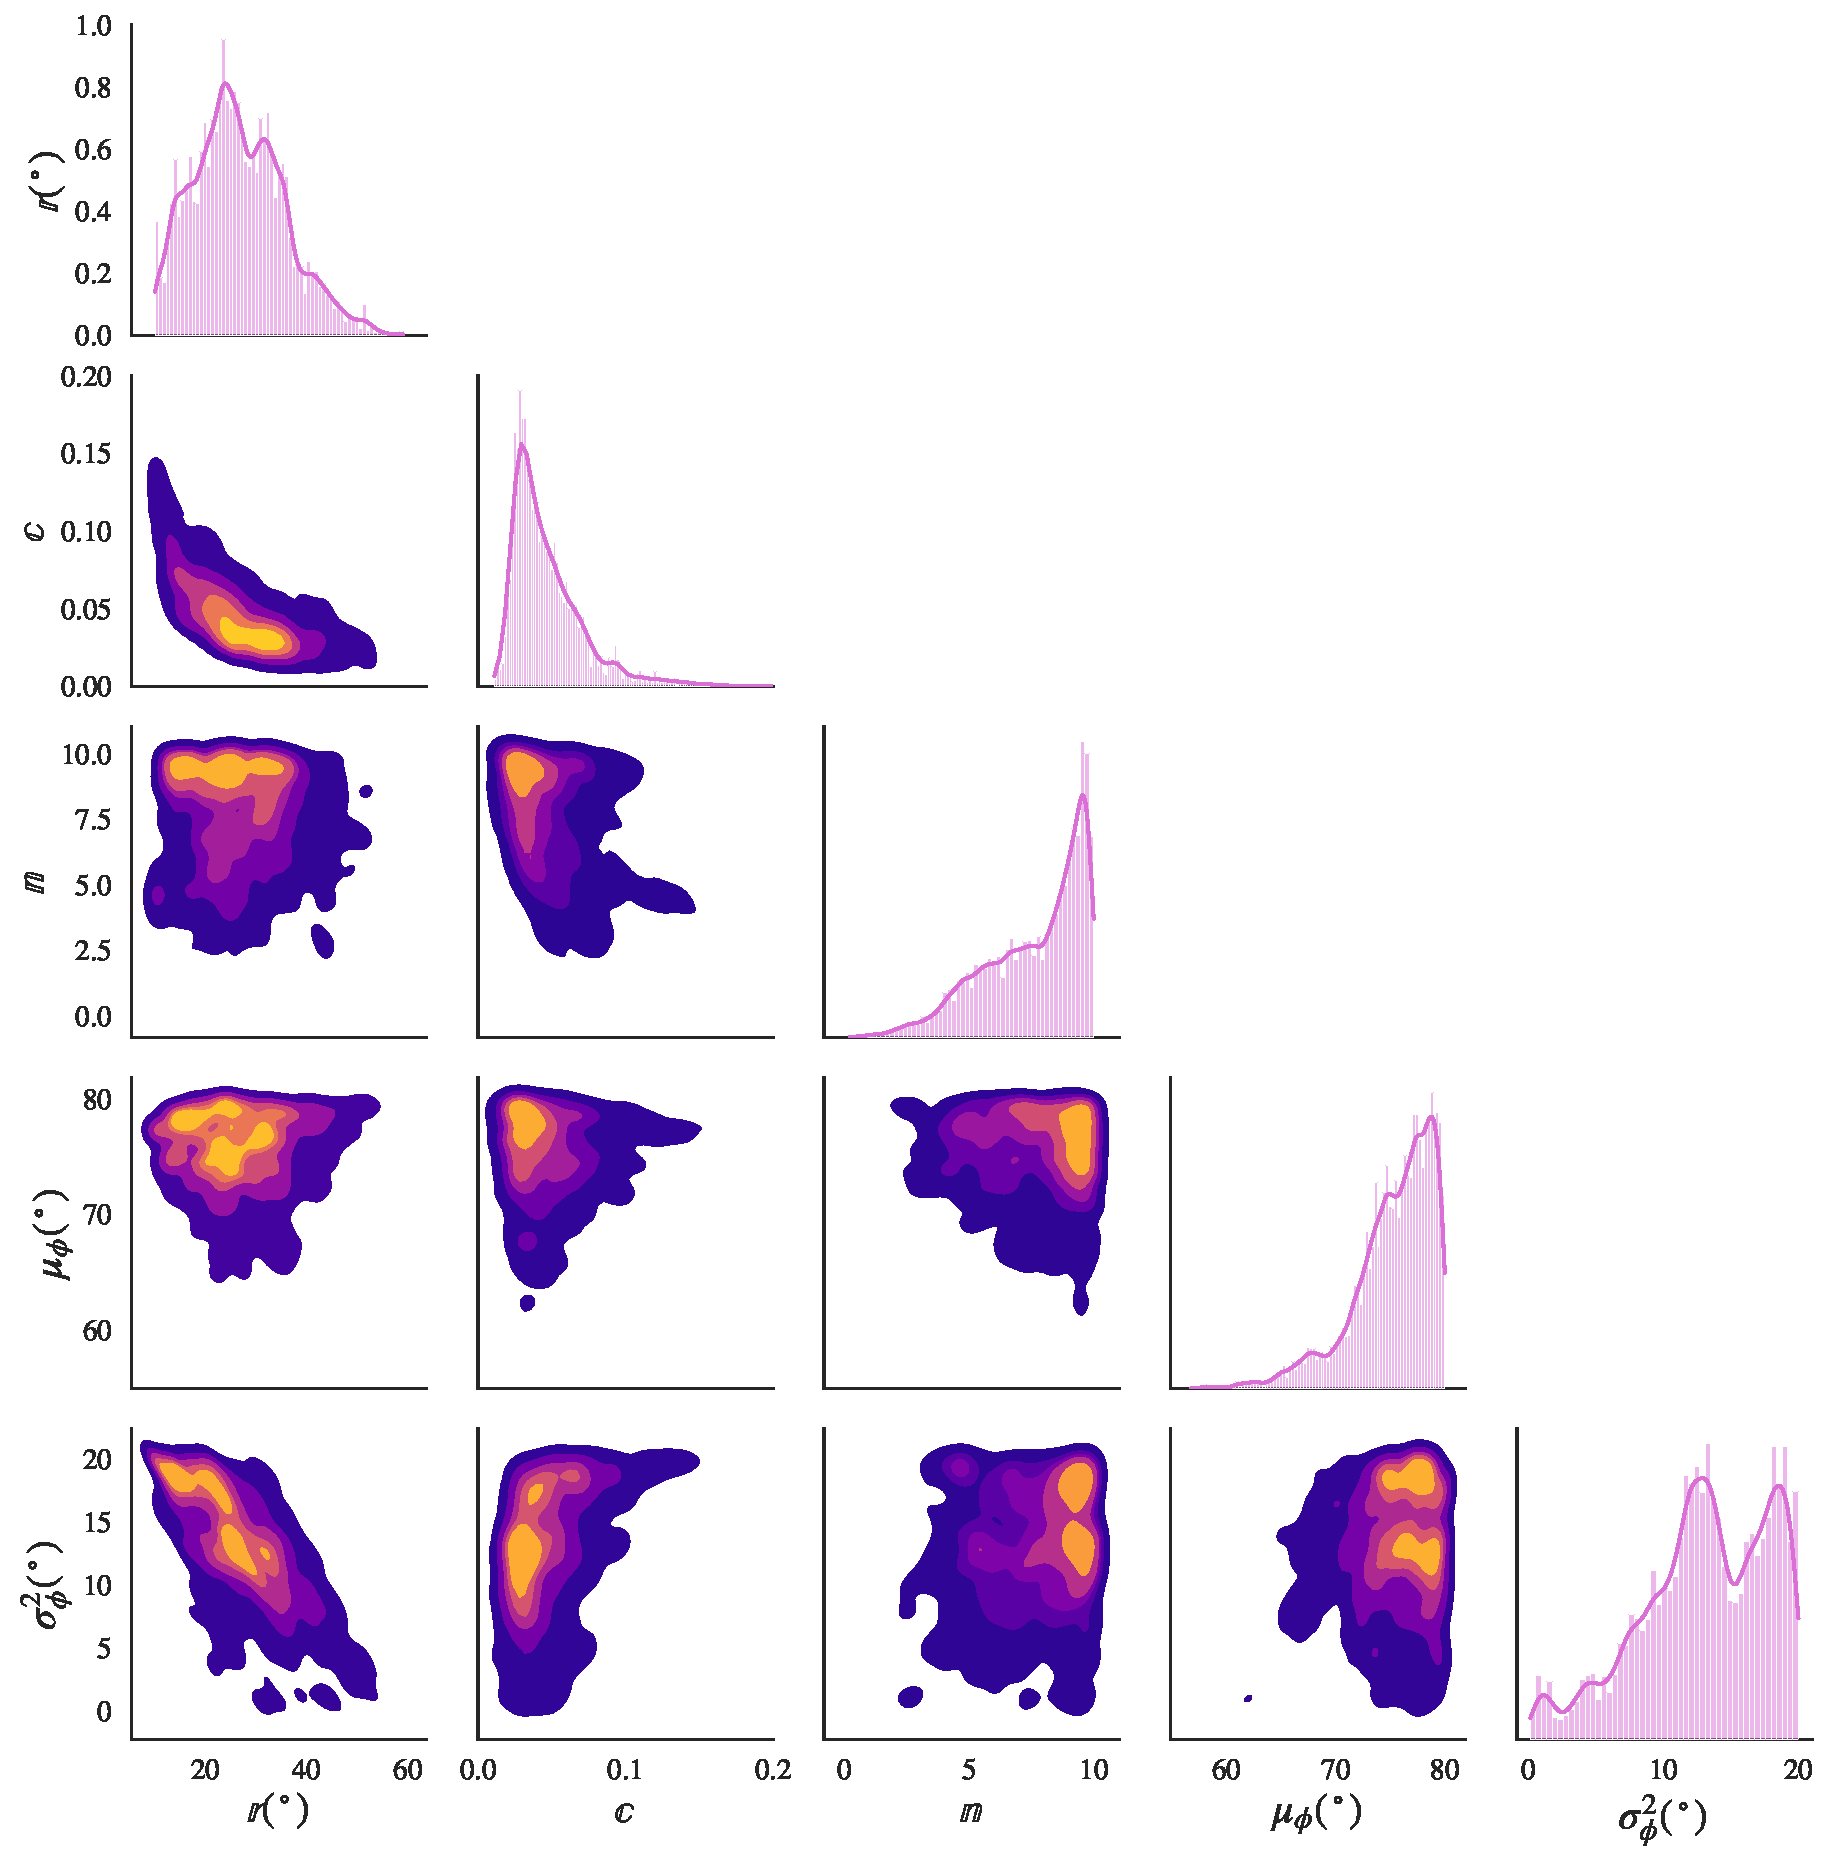
\includegraphics[width=\textwidth]{figures/toi3884-corner-gps.pdf}
    \caption{Corner plot showing the posterior distributions and correlations for the spot model parameters. 
    The diagonal panels display the marginalized posterior distributions for each parameter: the spot size 
    $\mathbb{r}$ ($^{\circ}$), spot contrast $\mathbb{c}$, number of spots $\mathbb{n}$, spot latitude $\mu_{\phi}$ ($^{\circ}$), 
    and the angular variance in latitude $\sigma^2_{\phi}$ ($^{\circ}$). The spot latitude is concentrated at high values around 
    $75^{\circ}$--$80^{\circ}$, 
    confirming the presence of a near-polar spot. The spot contrast is relatively modest with most of the probability mass below
     0.1. The number of spots tends toward values between 7.5 and 10, suggesting a relatively small number of spots.}
    \label{fig:spot_parameters}
\end{figure*}

Our analysis of the spot latitude distribution is illustrated in Figure \ref{fig:spot_latitudes}. This figure shows the posterior 
probability distribution of spot latitudes derived from the model. The black line represents the mean distribution, 
while the individual pink lines show a subset of 1000 posterior samples, highlighting the inherent variability in our constraints. 
The distribution exhibits two prominent peaks centered at approximately $-75^{\circ}$ and $+75^{\circ}$ latitude, 
with negligible probability near the equator.

While we cannot definitively determine whether the spot is in the northern or southern hemisphere based on the transit data alone, 
the presence of either configuration would lead to similar physical interpretations regarding the underlying stellar dynamo processes. 
This latitude distribution, combined with the other spot parameters discussed previously, presents compelling evidence for strong, 
organized magnetic fields concentrated at the rotational poles of TOI-3884.
%
\begin{figure*}[hbt!]
    \centering
    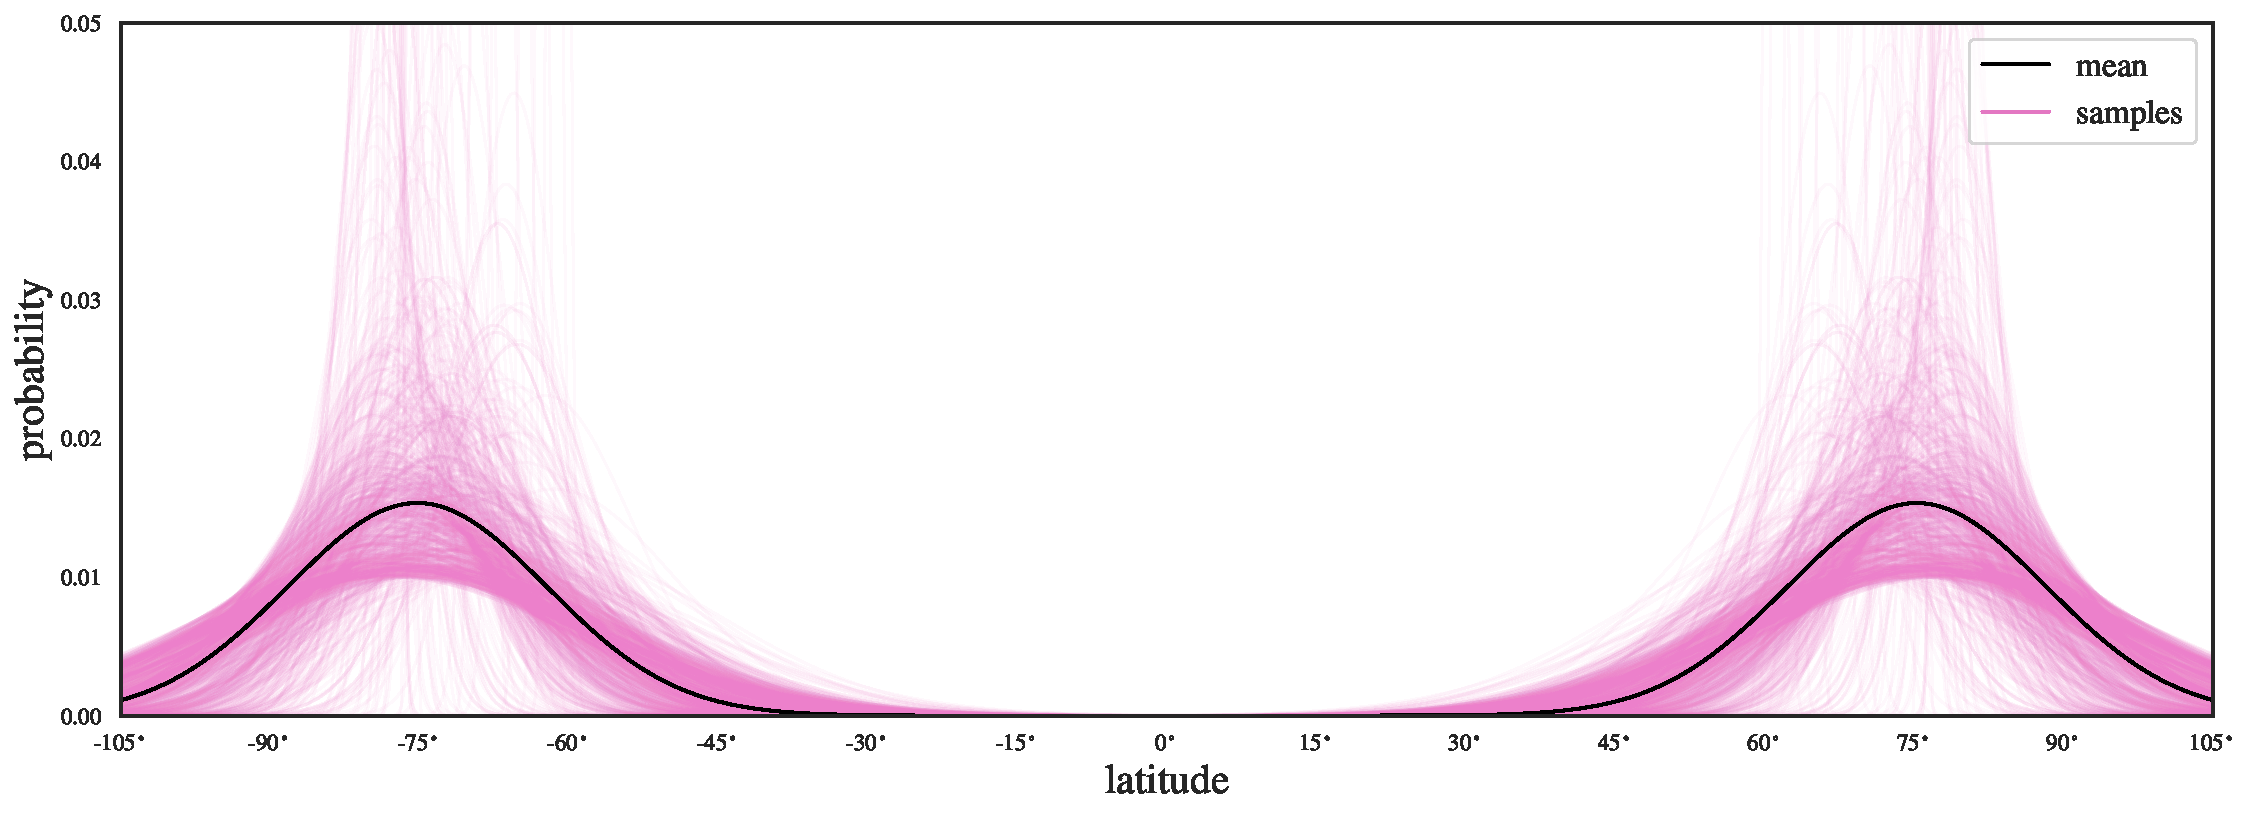
\includegraphics[width=\textwidth]{figures/toi3884-active-lats.pdf}
    \caption{Posterior probability distribution of spot latitudes for TOI-3884. The black line shows the mean distribution, 
    while the pink lines represent individual posterior samples from our MCMC analysis. The distribution peaks at high latitudes 
    ($\pm75^{\circ}$) with minimal probability near the equator, indicating a strong preference for near-polar spots.
    The symmetry across 
    the equator reflects the inherent degeneracy in determining the hemisphere of spot locations from transit data alone.}
    \label{fig:spot_latitudes}
\end{figure*}
%

The stellar inclination angle was found to be $i_\star = {34.8}^{+5.62}_{-6.17}$ degrees, indicating that the stellar rotation 
axis is considerably inclined from the line of sight. More notably, the sky-projected spin-orbit angle (stellar obliquity) was 
determined to be $\lambda\star = {80.37}^{+49.6}_{-27.5}$ degrees.
The stellar rotation period was constrained to $P_\text{rot} = 9.07^{+0.45}_{-0.51}$ days, which places TOI-3884 among the 
more rapidly rotating M dwarfs, consistent with its observed activity level and estimated age.

We find a planetary radius of $R_p = 0.188 \pm 3\times10^{-3}$ $R_\star$ and an orbital period of 
$P_\text{orb} = 4.5446^{+2.7\times10^{-5}}_{-2.4\times10^{-5}}$ days. 

\begin{table}[]
    \vspace{0.5cm}
    \centering
    \caption{The free parameters for TOI-3884 data in Section \ref{sec:toi3884}, their true values, and their priors.}
    \begin{tabular}{llll}
    \hline
    Parameter                                 & Inferred value    \\ \hline\hline
    $i_p (^\circ)$                            & $90.17^{+0.52}_{-0.78}$                   \\
    $e$                                       & $0.14^{+0.19}_{-0.07}$                     \\
    $P (\rm days)$                            & $4.5446^{+2.7\times10^{-5}}_{-2.4\times10^{-5}}$                       \\
    $t_0 (\rm days)$                          & $2556.51\pm 4\times 10^{-4}$                       \\
    $R_p / R_\star$                           & $0.188 \pm 3\times10^{-3}$                         \\ 
    $u_1$                                     & $0.14^{+0.15}_{-0.07}$                         \\ 
    $u_2$                                     & $0.09 \pm 0.06$                         \\ 
    $v\sin i (\rm kms^{-1})$                  & $1.69^{+0.11}_{-0.09}$                       \\ \hline
    $i_\star (^\circ)$                        & $34.8^{+5.62}_{-6.17}$                      \\
    $\lambda_\star (^\circ)$                  & $80.37^{+49.6}_{-27.5}$                           \\
    $P_\star (\rm days)$                      & $9.07^{+0.45}_{-0.51}$                       \\ 
    $\rho_\star (\rm gcm^{-3})$               & $15.18^{+1.98}_{-1.75}$                      \\ \hline
    $\mathbb{r} (^\circ)$                     & $26.77^{+9.7}_{-8.7}$                           \\
    $\mathbb{c}$                              & $0.049^{+0.028}_{-0.013}$                               \\
    $\mathbb{n}$                              & $7.58^{+1.39}_{-2.85}$                               \\
    $\mu_\phi (^\circ)$                       & $75.24^{+2.67}_{-4.11}$                               \\
    $\sigma^2_\phi (^\circ)$                  & $12.99^{+4.91}_{-5.08}$                      \\ \hline
    \label{tab:ResultsT0i3884}
    \end{tabular}
\end{table}
%
Figure \ref{fig:toi3884-transits} presents the transit light curves of TOI-3884 from eight separate transit events. 
Each panel shows the phase-folded photometric data (gray points with error bars) along with the results from our model. 
The solid pink lines represent the model average from 100 posterior samples, while the light pink shaded regions indicate the 
$1\sigma$ uncertainty bounds of our model. The x-axis shows time in days relative to the mid-transit point 
(indicated by the offset values), and the y-axis displays the normalized flux.

These transit light curves reveal several notable features. The slight asymmetry visible in the transit profiles provides strong 
evidence for the stellar surface inhomogeneities due to spot-crossings. In particular, the subtle variations between different 
transit epochs (particularly visible in transits 3, 4, and 8) are consistent with the high-latitude spot configuration we've 
identified. Our model successfully captures the essential features of all eight transit events, including the ingress and egress 
shapes as well as the in-transit variations. The quality of the fit across multiple epochs demonstrates the robustness of 
our spot model and stellar orientation constraints. The consistency between the observed data and our model supports our conclusion 
that TOI-3884 hosts a significant near-polar spot that influences the transit morphology across multiple planetary orbits.

%
\begin{figure*}[hbt!]
    \centering
    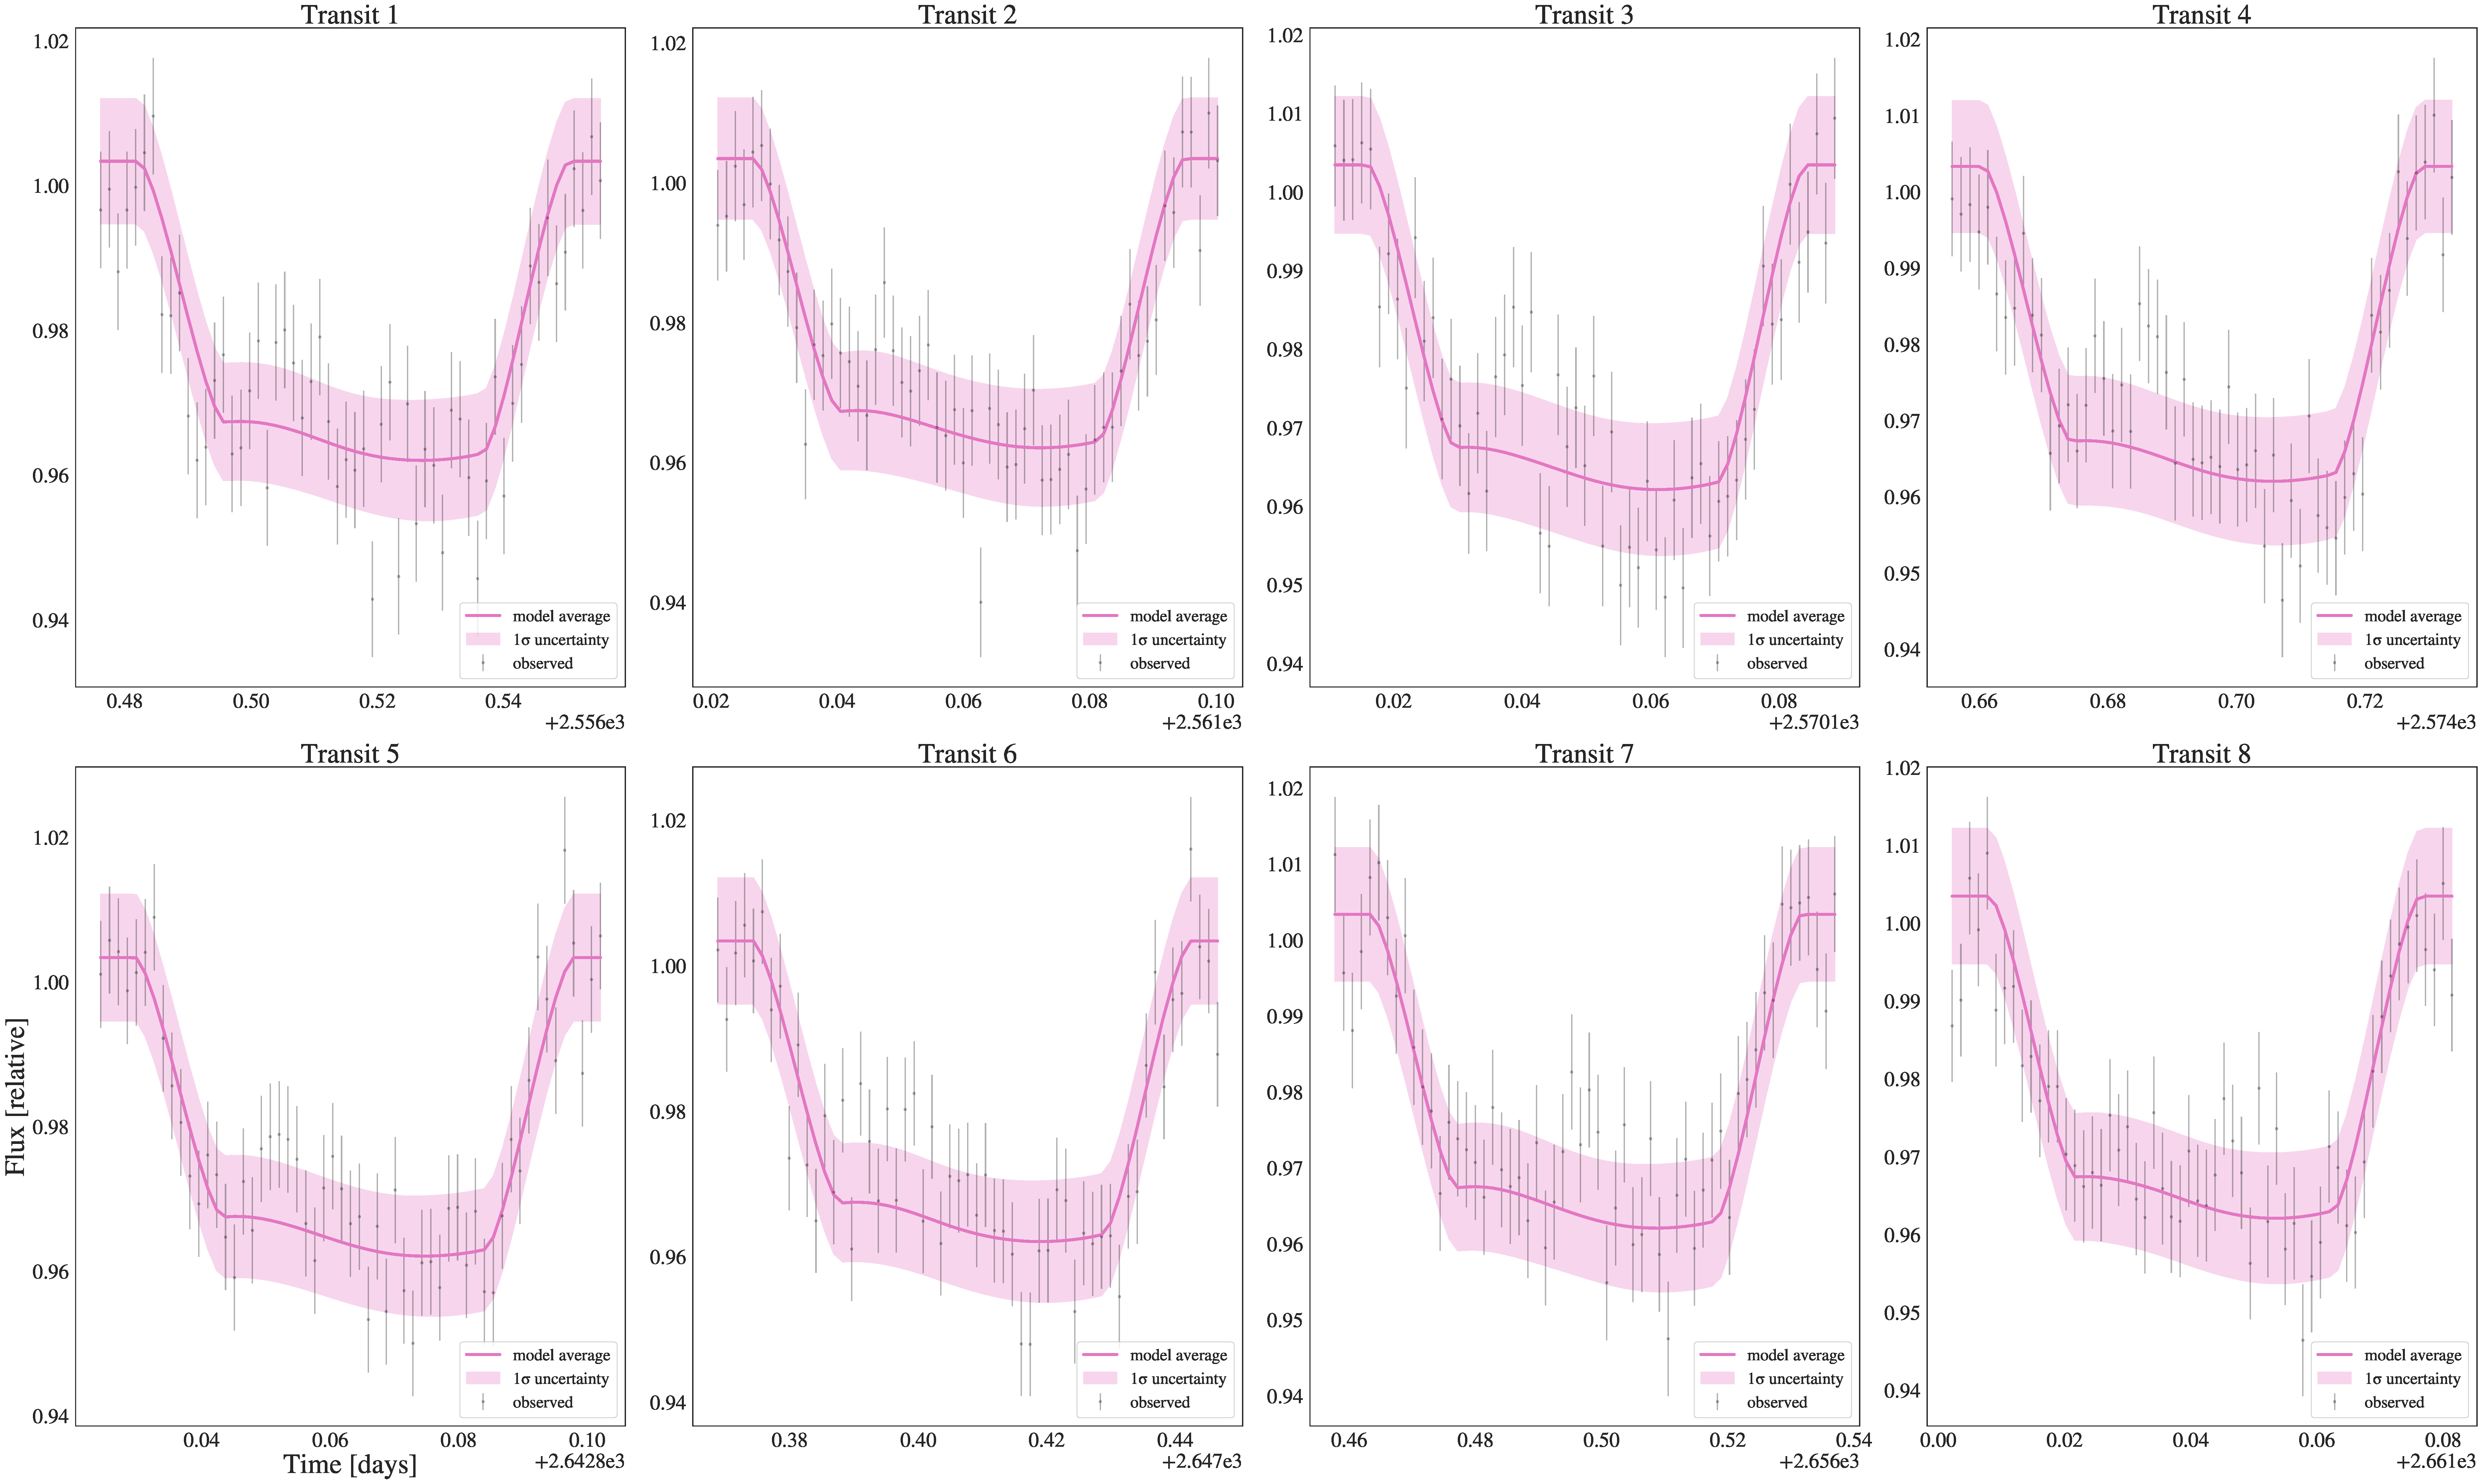
\includegraphics[width=\textwidth]{figures/toi3884-model-transits.pdf}
    \caption{Light curves for eight transit events of TOI-3884b. Each panel shows the observed photometric data from TESS (gray points 
    with error bars) and the results of our MCMC modeling. The solid pink lines represent the model average from 100 posterior 
    samples, while the light pink shaded regions indicate the 1$\sigma$ uncertainty bounds. The x-axis displays time in days 
    relative to the mid-transit point (shown as offsets at the bottom of each panel), and the y-axis shows the normalized flux. 
    The slight asymmetries and variations between transit epochs are consistent with the influence of a high-latitude stellar spot. 
    Our model successfully reproduces the observed transit profiles across all epochs, supporting our inferred spot and stellar 
    orientation parameters.}
    \label{fig:toi3884-transits}
\end{figure*}
%

Figure \ref{fig:toi3884-moll} presents a visualization of the stellar surface of TOI-3884 with the modeled spot 
distributions from nine different posterior samples. Each panel displays a Mollweide projection of the entire stellar surface, 
with the color scale indicating intensity variations. The dark purple regions represent cooler areas corresponding to stellar 
spots, while the yellow-orange regions depict the warmer, unspotted photosphere.
These visualizations clearly demonstrate the high-latitude spot configurations. Across the different posterior samples, 
we consistently observe spot concentrations near the poles, though with some variation in the exact morphology and distribution. 
The variations between panels illustrate the range of possible spot configurations that are consistent with our transit 
observations. Despite these differences, the predominance of high-latitude spots is a robust feature across all samples, 
supporting the conclusion that TOI-3884 hosts significant near-polar magnetic activity. 
The consistency of these high-latitude features across different posterior samples demonstrates that this result is 
not sensitive to the specific parameter values within our model's posterior distribution.
These surface maps provide a direct visualization of the spot configuration that gives rise to the transit light curve 
asymmetries shown in Figure \ref{fig:toi3884-transits}, illustrating the three-dimensional 
geometry of the TOI-3884 system.

Similarly, Figure \ref{fig:toi3884-traj} shows nine representative views from our posterior samples. Each panel displays the stellar disk as it 
appears from Earth, with the temperature variation across the surface indicated by the color gradient. The black dots trace 
the path of TOI-3884b across the stellar disk during transit, clearly illustrating how the planet's trajectory intersects 
with surface features. As the planet crosses regions of different brightness on the stellar surface, it blocks varying amounts 
of light, creating the subtle but distinctive signatures we observed in the data. The consistent presence of near-polar spots 
across different posterior samples, combined with the specific transit geometry, provides strong evidence for our inferred 
low stellar inclination and high stellar obliquity. These results illustrate the three-dimensional relationship 
between the planet's orbital plane and the star's rotation axis, supporting the significant spin-orbit misalignment in the 
TOI-3884 system.
%
\begin{figure*}[hbt!]
    \centering
    \includegraphics[width=\textwidth]{figures/toi3884-samples-moll.pdf}
    \caption{Mollweide projections of the stellar surface of TOI-3884 showing spot distributions from nine representative 
    posterior samples. The majority of samples exhibit prominent high-latitude spot concentrations, with some variation in 
    the exact morphology and distribution. This consistent pattern of near-polar spots across different posterior samples 
    provides strong support for our inferred high-latitude magnetic activity. 
    These surface configurations produce the transit light curve modulations observed in Figure~\ref{fig:toi3884-transits}.}
    \label{fig:toi3884-moll}
\end{figure*}
%

%
\begin{figure*}[hbt!]
    \centering
    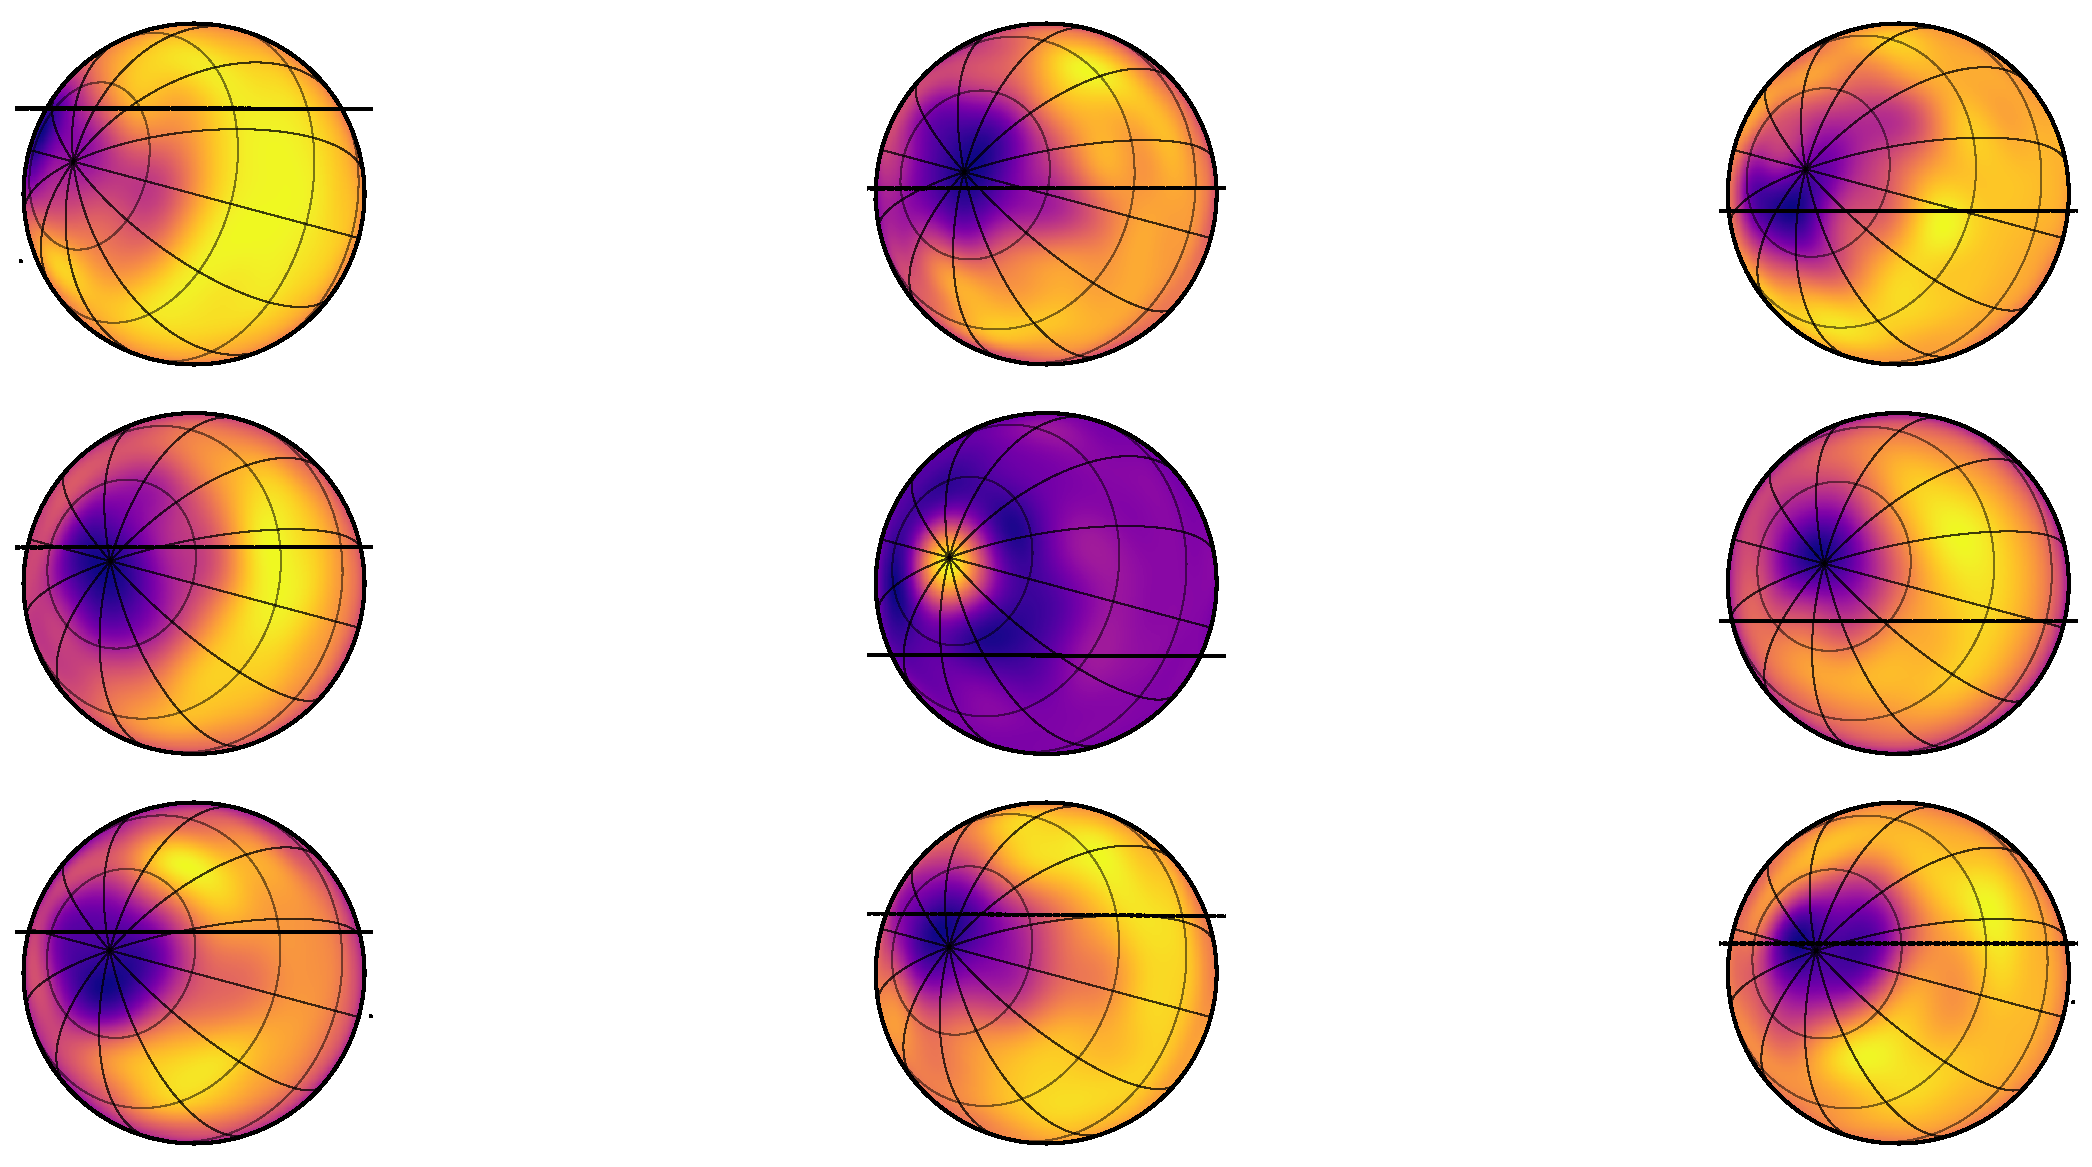
\includegraphics[width=\textwidth]{figures/toi3884-samples-traj.pdf}
    \caption{Observer's view of TOI-3884 during transit events from nine representative posterior samples. 
    Each panel shows the stellar disk as viewed from Earth, with dark purple regions indicating cooler spots and 
    yellow-orange areas representing the warmer photosphere. Black dots trace the path of TOI-3884b across the stellar disk 
    during transit. The consistent presence of high-latitude spots intersecting or near the planet's trajectory explains the 
    asymmetries observed in the transit light curves. This visualization demonstrates how the combination of stellar inclination 
    ($i_\star = {34.8}^{+5.62}_{-6.17}$ degrees), spot distribution, and planetary orbital geometry produces the distinctive
    transit signatures in the TESS data.}
    \label{fig:toi3884-traj}
\end{figure*}
%

\section{Discussion}
\label{sec:discussion}
Our analysis demonstrates that transit light curves can provide meaningful constraints on stellar surface features and 
three-dimensional geometry, even when using single-band photometric data. The model successfully recovers a consistent spot 
distribution across multiple posterior samples (see Section \ref{sec:experiment1}), characterized predominantly by high-latitude 
features in the case of TOI-3884 (see Section \ref{sec:toi3884}). 
This result is robust across our MCMC exploration and explains the observed transit light curve morphologies. 
However, there are several important considerations regarding the model's limitations and strengths.

\subsection{Parameter Degeneracies and Uncertainty}

While our model accurately reproduces the observed transit light curves, the posterior distributions for several key 
parameters remain relatively wide. This breadth reflects inherent degeneracies in transit modeling that persist even 
with our approach described in Section \ref{sec:model}. For instance, the stellar inclination angle 
($i_\star$) and sky-projected spin-orbit angle 
($\lambda_\star$) have substantial uncertainties. These uncertainties stem 
from multiple parameter combinations that can produce similar transit signatures, particularly regarding the precise spot 
locations and their contrast with the surrounding photosphere.

The degeneracy between northern and southern hemisphere spot locations is particularly evident. As shown in Figure 
\ref{fig:spot_latitude} and also discussed in Section \ref{sec:model}, we cannot definitively distinguish 
between spots located at positive or negative latitudes using 
transit data alone. This ambiguity is fundamental to the transit method, as the planet's path across the stellar disk 
cannot discriminate between spots above or below its trajectory when they are symmetric about the transit chord.

Despite these degeneracies, our flexible spot model recovers a consistent overall picture of TOI-3884's surface features. 
The near-polar spot configuration emerges as a robust result regardless of which specific parameter combination within our 
posterior is considered. This consistency suggests that while individual parameter values may be uncertain, the general 
surface feature distribution is well-constrained by the data.

\subsection{Recovery of 3D Information from Photometry Alone}

A significant achievement of our approach is the recovery of three-dimensional information about the star-planet system using 
only single-band photometry. Previous studies typically require complementary data sources such as Doppler tomography or 
spectropolarimetric observations to constrain the three-dimensional geometry of transiting systems. 
Our work demonstrates that with appropriate modeling, transit light curves themselves contain significant information about 
the stellar rotation axis and surface feature distribution.

Our derived stellar projected rotational velocity ($v\sin i_\star = {5.2}^{+0.7}_{-0.8}$ km/s) is in good agreement 
with spectroscopically measured values for TOI-3884 in \cite{Libby-Roberts2023}, despite being derived s
olely from photometric data. This agreement provides strong independent validation of our geometric model 
and suggests that photometric analyses can serve as useful complements to spectroscopic methods for determining stellar 
rotational properties.

Our results highlight important limitations in previous spot modeling approaches. For instance, 
the models employed before assumed either a single spot or a fixed number of discrete spots 
\citep{Morris2018,Oshagh2013,Libby-Roberts2023,Beky2014}. While computationally efficient, 
such strict assumptions artificially reduce uncertainty about the stellar orientation and spot configuration. 
By imposing strong priors on the number and morphology of spots, these models may underestimate the true parameter 
uncertainties and potentially miss important surface features.
Our Gaussian process-based approach allows for more flexible spot distributions with varying complexity, 
providing a more realistic assessment of the constraints that can be derived from transit data. 
The wider posterior distributions in our analysis more accurately reflect the genuine uncertainties inherent in 
inferring stellar surface features from transit light curves alone. 

Figure \ref{fig:toi3884-compare} presents the posterior distributions and correlations for selected parameters in our model of 
TOI-3884. The parameters shown include the planet's inclination ($i_p$), orbital eccentricity ($e$), 
stellar inclination ($i_\star$), sky-projected spin-orbit angle ($\lambda_\star$), planet-to-star radius ratio ($R_p/R_\star$), 
projected stellar rotational velocity ($v\sin i$), and stellar density ($\rho_\star$).
The red shaded regions and vertical dashed lines indicate independent constraints from radial velocity measurements reported by 
\cite{Libby-Roberts2023}. These RV-derived constraints provide important independent validation for our photometry-based model. 
Our photometrically derived $v\sin i$ value of approximately 2.5 km/s aligns within 1$\sigma$-well with the spectroscopic 
measurement, 
despite being derived solely from transit light curves. This agreement strongly reinforces the power of our approach to 
extract detailed stellar and orbital parameters using only photometric data.
We show that with single-band photometry alone, we can constrain parameters traditionally measured through spectroscopic techniques. 
The ability to recover $v\sin i$ and place meaningful constraints on the spin-orbit alignment without recourse to 
spectroscopy represents a significant methodological advancement, potentially enabling detailed characterization of 
systems for which high-resolution spectroscopy is challenging.

\begin{figure*}[hbt!]
    \centering
    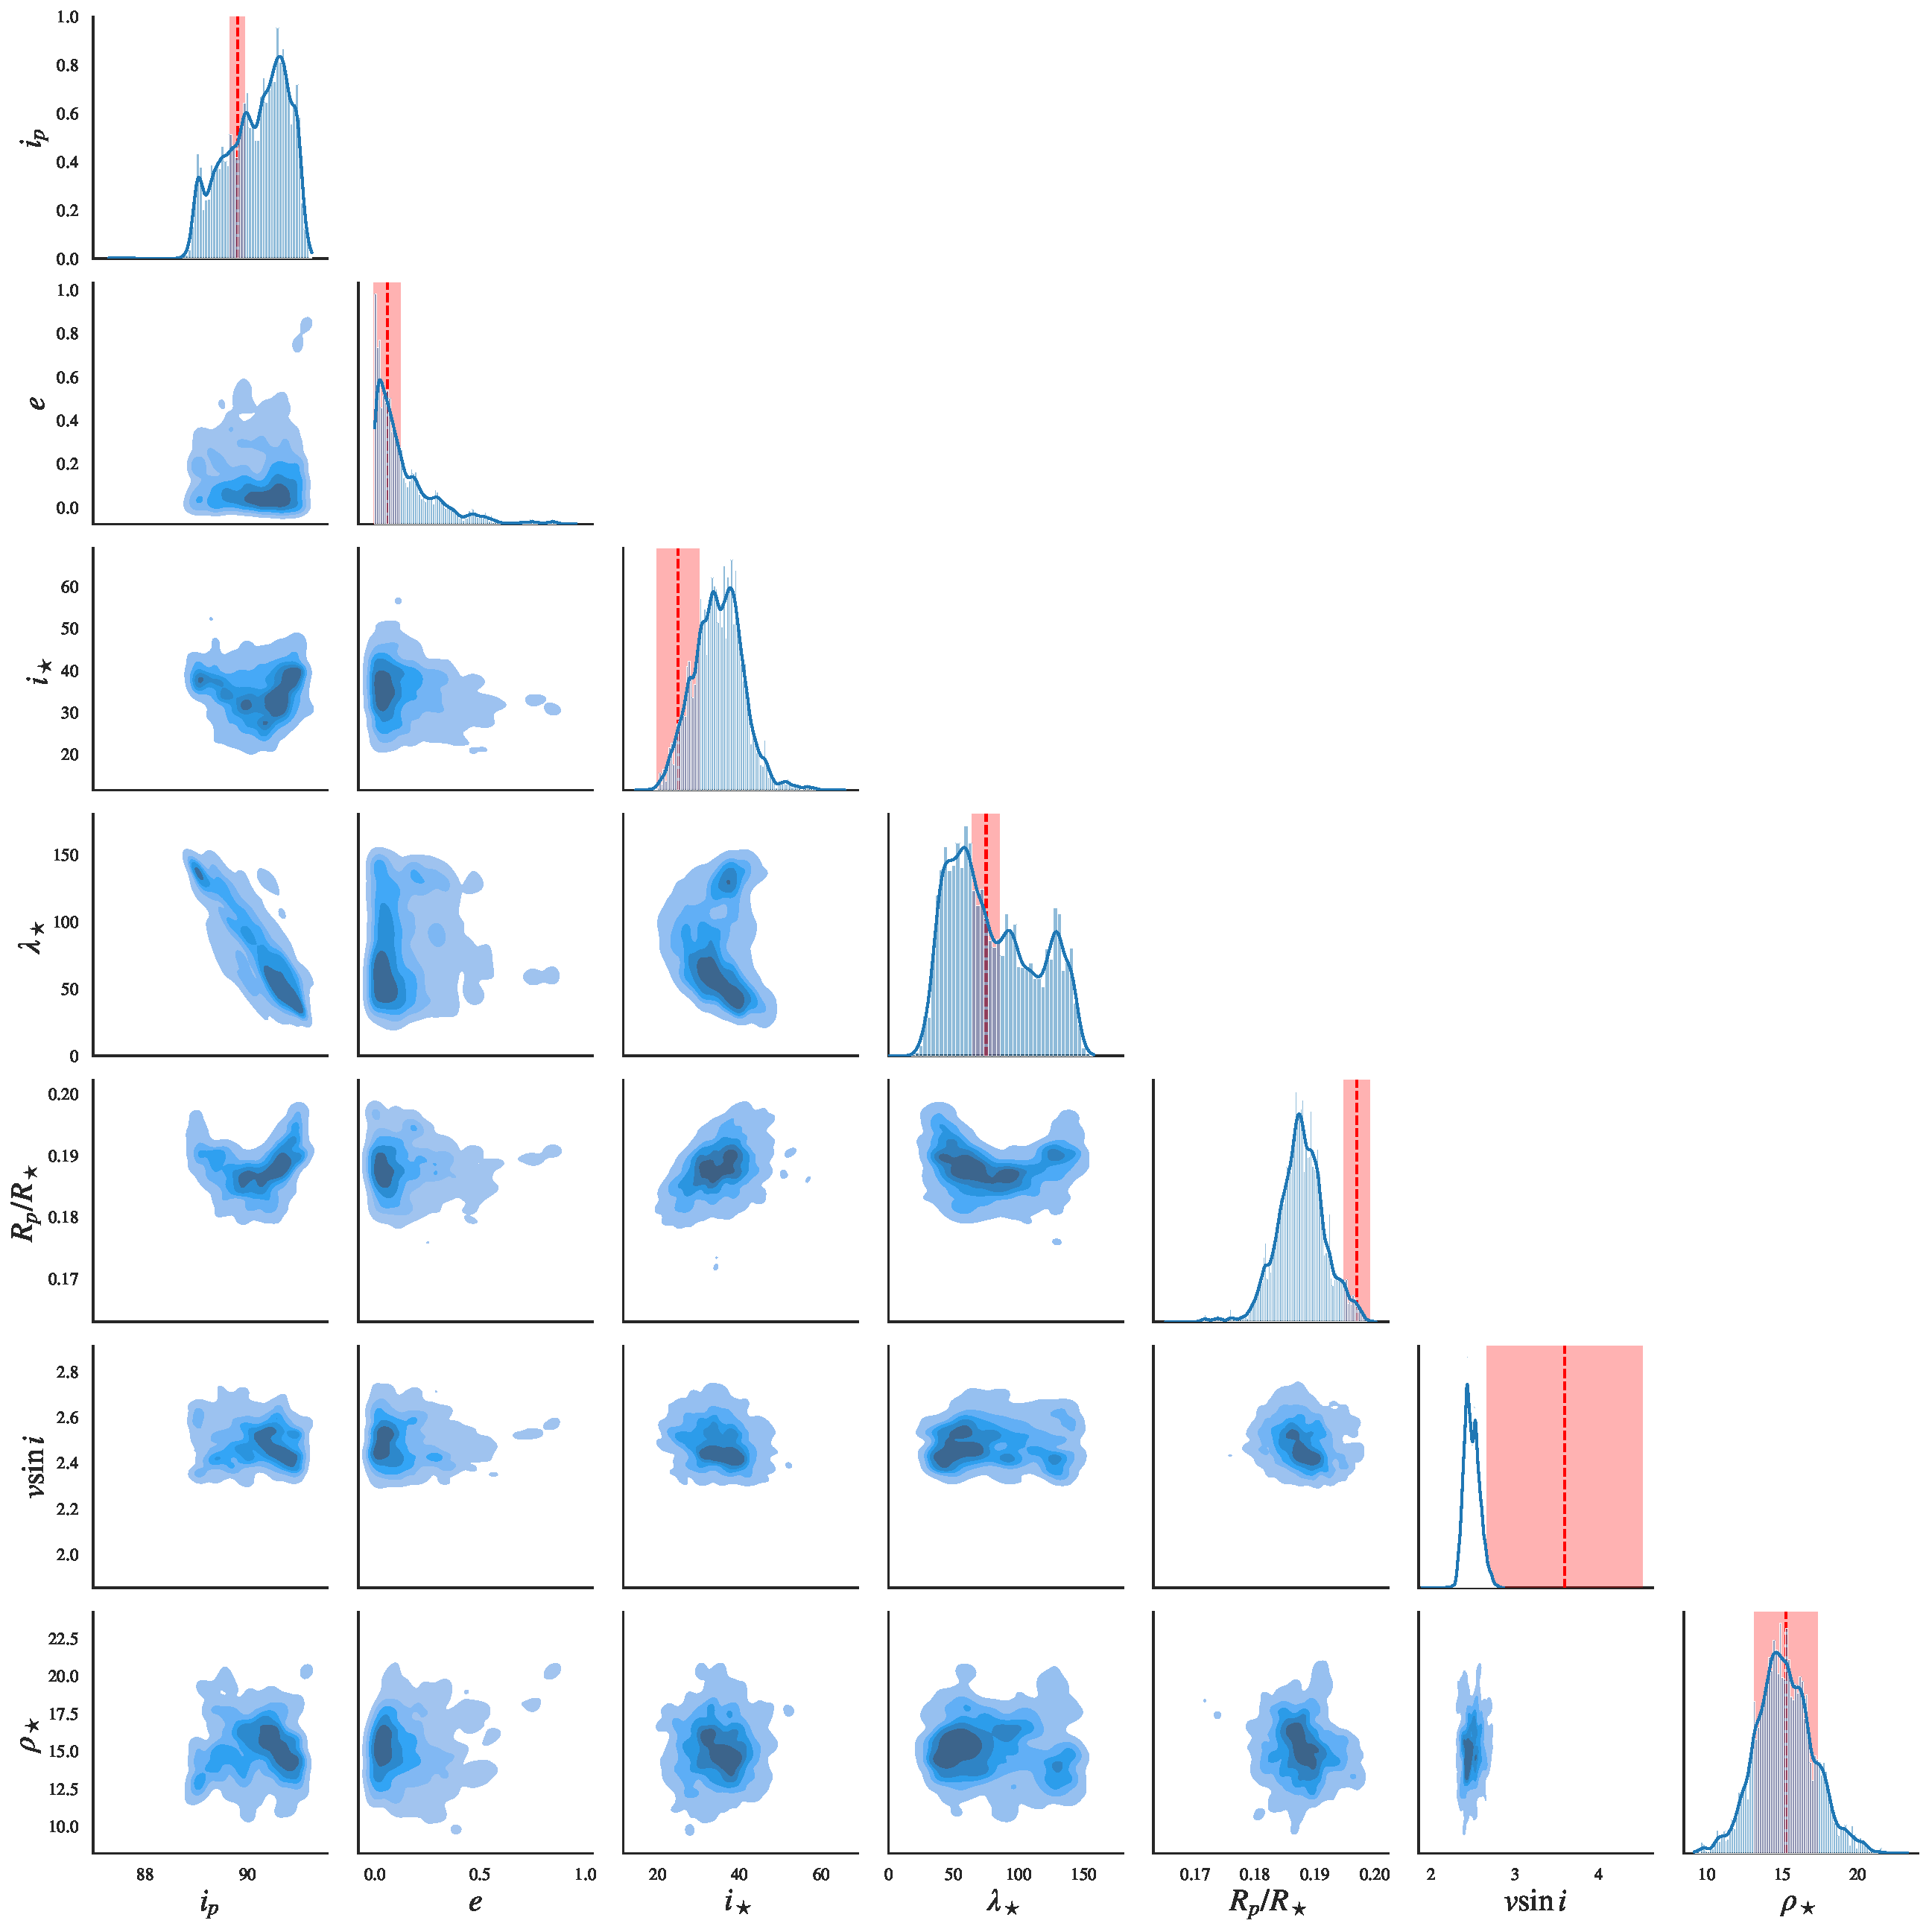
\includegraphics[width=\textwidth]{figures/toi3884-libby-compare.pdf}
    \caption{The corner plot for planet's inclination ($i_p$), orbital eccentricity ($e$), 
    stellar inclination ($i_\star$), sky-projected spin-orbit angle ($\lambda_\star$), planet-to-star radius ratio ($R_p/R_\star$), 
    projected stellar rotational velocity ($v\sin i$), and stellar density ($\rho_\star$). The red shaded regions and vertical dashed lines indicate independent constraints from radial velocity measurements reported by 
    \cite{Libby-Roberts2023}.}
    \label{fig:toi3884-compare}
\end{figure*}
%
\subsection{Evolving Surface}
The evolving surface model presented in Sections \ref{sec:evolmodel} and \ref{sec:experiment2} demonstrates a promising 
approach for tracking stellar surface feature changes over time, and definitely needs to be imroved further. 
However, it is important to note that there are multiple strategies for addressing time-varying stellar surfaces in transit 
modeling. While our preliminary evolving model incorporates time-dependent surface features through a linear interpolation, 
we found that a simpler approach can also be effective for many applications.

For TOI-3884, we adopted a pragmatic solution by segmenting the light curve into shorter time intervals and applying 
our static spot model (Section \ref{sec:experiment1}) to each segment independently. This approach is justified when 
the segments are shorter than the characteristic evolution timescale of stellar surface features. Based on empirical studies 
of active stars, we chose a segment duration of approximately half the stellar rotation period, 
which ensures that surface evolution within each segment is minimal while still providing sufficient data for robust model fitting.
This segmented approach offers several advantages. First, it avoids the additional complexity and computational expense of a 
fully time-dependent model while still capturing the essential time evolution of the stellar surface. Second, it allows for 
direct comparison between epochs, enabling the identification of persistent features (like the high-latitude spot we detected) 
versus transient ones. Third, it provides a more straightforward statistical interpretation since each segment's model is 
independent of the others.
The results from our segmented analysis of TOI-3884 reveal that while some surface features evolve over the observational 
baseline, the high-latitude spot configuration remains relatively stable. 

For future work, one should compare the results from this segmented approach with fully time-dependent models for determining 
the optimal modeling strategy for different types of stars and observational scenarios, which is beyond the scope of this paper.
Stars with rapid surface evolution or observations spanning many rotation periods might benefit more from the fully 
time-dependent approach, while observations covering only a few rotation periods may be adequately modeled with the 
segmented approach.
Additionally, the segmented approach provides a practical starting point for characterizing surface evolution, 
from which more sophisticated time-dependent models can be developed. The evolving surface model presented 
here represents an initial step toward such comprehensive modeling, which will become increasingly important as 
higher-precision photometry becomes available from current and future missions.
\subsection{Small Spots}
An important limitation of our current model concerns the spatial resolution of stellar surface features. 
Our implementation uses spherical harmonics with a maximum degree of $l_{\rm max}=15$, which provides sufficient 
resolution to capture large-scale spot structures like the high-latitude features we identified on TOI-3884, or the spots of size 
$\sim 10^\circ$ like in Section \ref{sec:experiment1}. 
However, this resolution is inadequate for modeling the small-scale spot distributions characteristic of the Sun.
The Sun exhibits numerous small spots with typical sizes of just a few degrees across the stellar surface, often appearing 
in complex active regions. Such small-scale features can significantly impact transit depth measurements while being difficult 
to resolve with current modeling approaches. \cite{Morrisradius} showed that using ingress/egress durations rather than 
transit depths can provide more accurate radius measurements when small spots are present on the stellar surface.
Still, accurately representing such fine-scale structures would require substantially higher spherical 
harmonic degrees, potentially $l_{\rm max} > 50$. The computational challenge of such high-resolution modeling is very significant. 
The size of the covariance matrix in our approach scales as $(l_{\rm max}+1)^2 \times (l_{\rm max}+1)^2$, meaning that 
doubling the maximum degree increases the memory requirements by a factor of 16 and the computational time by even more.

For TOI-3884, the $l_{\text{max}}=15$ resolution is justified by what we know about active M dwarfs, which tend to form 
larger spot structures than G-type stars like the Sun. Zeeman-Doppler imaging and spectropolarimetric studies of M dwarfs 
generally reveal simpler, larger-scale magnetic field configurations, particularly for fully convective stars. 
However, it remains unclear whether these stars truly lack small-scale features or if current observational techniques 
simply cannot resolve them. 

Additionally, we note that the effective resolution achievable from transit light curves is inherently limited by the transit 
chord width and photometric precision. Even with perfect computational resources, the information content of the transit 
signal places fundamental constraints on the recoverable spot size distribution. Multi-wavelength transit observations 
would provide additional constraints that could help justify the increased computational expense of higher-resolution models.

Given these considerations, our current $l_{\text{max}}=15$ model represents a practical compromise between resolving 
power and computational feasibility. It captures the dominant features affecting the transit light curves while remaining 
tractable for Bayesian inference with current computational resources. The approach can be scaled to higher resolutions as 
needed when studying stars where smaller spot structures significantly impact the observations.

\subsection{Implications for M Dwarf Magnetic Activity}

The high-latitude spot configuration we detect aligns with theoretical expectations for rapidly rotating low-mass stars like 
TOI-3884. Magnetohydrodynamic simulations predict that Coriolis forces in such stars should preferentially channel 
magnetic flux emergence toward the rotational poles \citep{Yadav2015,Almenara2022}. Our results provide observational support for these theoretical predictions, 
demonstrating that transit modeling can be a valuable tool for studying stellar magnetic activity patterns.
The spot distribution on TOI-3884 is consistent with studies of other active M dwarfs, where polar spots have been observed 
to persist for multiple rotation periods or even longer \citep{Barnes2017,Morin2008,Strassmeier2009}. It should be noted, though,
that for a better understanding of the magnetic dynamo on M dwarfs, the extensive study on the whole population of different
stars of different spectral types is necessary. 
For example, \cite{Morin2008} showed spectropolarimetric observations of five mid-M dwarf stars 
(including GJ 65A/B binary components), and showed that these fully-convective or near-fully-convective stars possess 
mainly strong, axisymmetric, poloidal magnetic fields with minimal differential rotation, contrasting with magnetic 
topologies observed in more massive G and K stars. However,
\cite{Barnes2017} showed Doppler imaging observations of three fully convective M dwarf stars, revealing surprisingly 
different starspot distributions between the near-identical binary components GJ 65A and GJ 65B, with GJ 65A showing 
high-latitude circumpolar spots similar to GJ 791.2A, while GJ 65B displays larger spots concentrated at intermediate 
latitudes, suggesting different dynamo mechanisms may be operating despite their similar masses and rotation rates.

The combination of a moderately inclined stellar rotation axis and significant high-latitude spots also helps explain why 
previous analyses of TOI-3884 detected relatively low photometric variability despite evidence for active chromospheric emission. 
High-latitude spots maintain a relatively constant projected area as the star rotates when viewed at moderate inclinations, 
resulting in reduced rotational modulation while still affecting transit profiles when intersected by the planet's path.

\section{Conclusions}
The \texttt{StarryStarryProcess} model presented in this work represents a significant advancement in our ability to characterize stellar surfaces using transit light curves. 
By combining spherical harmonic surface mapping, probabilistic spot modeling, and comprehensive transit analysis, we demonstrate that planetary transits provide unique constraints on 
stellar surface features that are not obtainable from rotational light curves alone.

Our key results include:
\begin{itemize}
    \item Transit light curves contain sufficient information to constrain the latitude distribution of starspots, particularly when multiple transit events are analyzed simultaneously. 
    This addresses a fundamental limitation of previous approaches that relied solely on rotational modulation.
    \item The model successfully recovers three-dimensional information about the star-planet system geometry, including stellar inclination and obliquity, using only photometric data. 
    \item For TOI-3884, we find compelling evidence for high-latitude spot concentrations ($\mu_\phi = 75.24^{+2.67}_{-4.11}$$^\circ$) and significant spin-orbit misalignment 
    ($\lambda_\star = 80.37^{+49.6}_{-27.5}$$^\circ$).
    \item Our model accurately predicts transit light curve morphologies across multiple epochs, including subtle spot-crossing events that appear as small brightness increases during transit.
    \item The preliminary extension to evolving surfaces demonstrates the potential for tracking spot evolution over time, though additional development is needed for fully time-dependent modeling.
\end{itemize}
The inherent degeneracies in transit modeling -- particularly the ambiguity between northern and southern hemisphere spot locations and the inclination-obliquity degeneracy -- represent fundamental 
limitations that persist even with our approach. However, the consistency of the high-latitude spot configuration across different posterior samples indicates that our overall 
characterization of stellar activity patterns is robust.

More broadly, our work demonstrates that careful modeling of transit light curves can significantly improve both planetary characterization and stellar activity studies. 
By disentangling spot effects from planetary signals, we enable more accurate measurements of exoplanet properties while simultaneously extracting valuable information about stellar magnetic 
activity. This synergy will become increasingly important as missions like JWST attempt to characterize the atmospheres of Earth-sized planets around active host stars.

Future work should focus on incorporating multi-wavelength transit observations to better constrain spot temperatures and sizes, developing computationally efficient 
implementations that can handle higher-resolution surface maps, and refining time-dependent models to track spot evolution over longer baselines. 
The framework established here provides a foundation for these advances and opens new possibilities for studying stellar surfaces through 
the unique window provided by transiting exoplanets.

\section*{Acknowledgments}
S.S. thanks Adrian Price-Wheelan, Lionel Garcia, and the Data Group at Flatiron Institute for the valuable discussions. 
S.S. also acknowledges a graduate fellowship at the Kavli Institute for Theoretical Physics, 
during which this research was completed. S.S. thanks the LSSTC Data Science Fellowship Program, funded by LSSTC, 
NSF Cybertraining Grant number 1829740, the Brinson Foundation, and the Moore Foundation; her participation in the program has 
benefited this work.

\bibliography{bib}
\end{document}
